\documentclass{wissdoc}

%% --------------------
%% |     Packages     |
%% --------------------

\usepackage[utf8]{inputenc}

% Weitere packages: (Dokumentation dazu durch "latex <package>.dtx")

%\usepackage{bibgerm}
%\usepackage[backend=biber]{biblatex} 
\usepackage{csquotes} 
\usepackage{tabularx}
\usepackage{booktabs}
\usepackage{multirow}
%\usepackage{tocbibind}
\usepackage{siunitx}
\usepackage{xcolor}
\usepackage{textcomp}
\usepackage{listings}
\usepackage{newfloat,caption}
\usepackage{subcaption}
\usepackage{footnote}
\usepackage{rotating}
\usepackage{pgfplots}
\usepackage{pgfplotstable}
\usepackage{url}
\usepackage{boxhandler}
\usepackage{tabu}
\usepackage{amssymb}
%\usepackage{subfig}
%\usepackage{subcaption}
\usepackage{caption}
\usepackage{subcaption}
%\usepackage[plainpages=true]{hyperref}
\usepackage[space]{grffile}
\usepackage{pdfpages}
%\usepackage[numbers,sort&compress]{natbib}
\usepackage[backend=bibtex,natbib=true,hyperref=true,doi=false,url=false]{biblatex}
% \usepackage{varioref}
% \usepackage{verbatim}
\usepackage{float}    %z.B. \floatstyle{ruled}\restylefloat{figure}
%\usepackage[hidelinks]{hyperref}
% \usepackage{subfigure}
% \usepackage{fancybox} % für schattierte,ovale Boxen etc.
% \usepackage{tabularx} % automatische Spaltenbreite
% \usepackage{supertab} % mehrseitige Tabellen
% \usepackage[svnon,svnfoot]{svnver} % SVN Versionsinformation 

% My packages
\usepackage{graphicx}


\usepackage{makeidx}%added by sajjad
\usepackage{fancyhdr}
\usepackage{enumitem}
\usepackage{titlesec}

%% --------------------
%% |     Settings     |
%% --------------------

% Settings: Titlepage, Comments, etc.
\pgfplotsset{compat=newest}

% Settings for Titlepage
\hypersetup{
	colorlinks,
  citecolor=black,
  filecolor=black,
  linkcolor=black,
  urlcolor=black,
 pdfauthor={FirstName LastName},
 pdftitle={Title of Thesis}
 pdfsubject={Not set},
 pdfkeywords={Not set}
}
\DeclareFloatingEnvironment[fileext=frm,placement={!ht},name=Listing,within=section]{listing}

% Print URLs not in Typewriter Font
\def\UrlFont{\rm}

\newcommand{\specialcell}[2][c]{%
  \begin{tabular}[#1]{@{}c@{}}#2\end{tabular}}

\newcommand\todo[1]{\textcolor{red}{TODO: #1}}

\newcommand\hlcode[1]{\textcolor{red}{#1}}

\newcommand\citeable[1]{\textcolor{green}{\hl{citeable: #1}}}

\newcolumntype{\$}{>{\global\let\currentrowstyle\relax}}
\newcolumntype{^}{>{\currentrowstyle}}
\newcommand{\rowstyle}[1]{\gdef\currentrowstyle{#1}%
  #1\ignorespaces
}

% Comments
\newif\ifcomment
%\commenttrue

% Leerseite ohne Seitennummer, nächste Seite rechts
\newcommand{\blankpage}{
 \clearpage{\pagestyle{empty}\cleardoublepage}
}

% Bibliography
\addbibresource{bib/references.bib}
\makeindex %added by sajjad
%% --------------------
%% |   STARTS Sajjad   |
%% --------------------
\usepackage{listings}
\usepackage{xcolor}
\definecolor{verbgray}{gray}{0.9}
\lstset{backgroundcolor=\color{verbgray},
	basicstyle=\scriptsize,
	frame=single,
	breaklines=true,
	postbreak=\mbox{\textcolor{red}{$\hookrightarrow$}\space},
}
%header and footer
\pagestyle{fancy}
\fancyhf{}
\fancyhead[LE,LO]{Customized Embedded Processors Design}
\fancyhead[RE,RO]{Tutorial}
\fancyfoot[LE,LO]{Sajjad Hussain CES KIT}
\fancyfoot[RE,RO]{Version 5:2022}
\fancyfoot[CE,CO]{\thepage}

\renewcommand{\headrulewidth}{2pt}
\renewcommand{\footrulewidth}{1pt}
\fancyheadoffset[RE,LO]{0pt}%adjusting the header/footer width https://latex.org/forum/viewtopic.php?t=7036
\fancyfootoffset[RE,LO]{0pt}
%remove the blank page after the title
\let\cleardoublepage=\clearpage%remove the blank page after the title
%Changing Sections, subsection, subsubsection Numbers to 1, 1.1, 1.1.1
\newtheorem{theo}[subsubsection]{Theorem}
\newtheorem{defi}[subsubsection]{Definition}
%Changing enumerate to 1.1 1.2 1.3
\renewcommand\theenumii{\theenumi.\arabic{enumii}}
\renewcommand\labelenumii{\theenumii} % LaTeX's default: "(\theenumii)"



%% --------------------
%% |   ENDS Sajjad    |
%% --------------------

%% --------------------------------------------------------------------------------
%% |                           BEGINNING OF DOCUMENT                              |
%% --------------------------------------------------------------------------------
\begin{document}

%% ----------------------
%% |     Title Page     |
%% ----------------------
%\frontmatter
%\pagenumbering{roman}

%% ----------------------------
%% |     Table of Content     |
%% ----------------------------
%\thispagestyle{empty}

%% ------------------
%% |     Content    |
%% ------------------

\graphicspath{{src/}}

\mainmatter
\pagenumbering{arabic}

%% Titelseite
%% Vorlage $Id: titelseite.tex 54 2009-12-10 12:23:58Z bless $

\def\usesf{}
\let\usesf\sffamily % diese Zeile auskommentieren für normalen TeX Font



\begin{titlepage}
\setlength{\unitlength}{1pt}

\begin{picture}(0,0)(85,770)
%
\includegraphics[width=\paperwidth]{src/logos/KIT_Deckblatt}
%added by sajjad

\includegraphics[width=\paperwidth]{src/logos/KIT_Deckblatt_CES1}
\end{picture}

%\vspace*{-39pt}\hspace*{260pt}\parbox[]{10cm}{\usesf Institute of Computer Engineering\\ Chair of Embedded Systems}
%added by sajjad
\vspace*{-39pt}\hspace*{160pt}\parbox[]{10cm}{\usesf KIT-Fakultät für Informatik \\ Institut für Technische Informatik}

\thispagestyle{empty}

%\begin{titlepage}
%%\let\footnotesize\small \let\footnoterule\relax
\begin{center}
\hbox{}
\vfill

{\usesf\large
{\huge\bfseries Tutorial - ASIPmeister Adding Resources}
\vskip 2.5cm

{\LARGE\bfseries Customized Embedded Processor Design}
\vskip 0.25cm

{\large\bfseries Application Specific Instruction-Set Processors- ASIP\\}
Lab (Prakitikum)
\vskip 1.5cm

Responsible/Author:  \\
{\large\bfseries MSc. Sajjad Hussain\\}

}
\end{center}
\vskip 3cm

\textbf{Supervisors:}  \\
{MSc. Sajjad Hussain,  Dr.-Ing. Lars Bauer, Prof. Dr.-Ing. Jörg Henkel\\}

\vskip 2cm
Chair of Embedded Systems,\\
Building 07.21, Haid-und-Neu-Str. 7, \\
76131 Karlsruhe, Germany. \\

\vskip 1cm
\rightline\today

\vfill
\end{titlepage}
%% Titelseite Ende
%\chapter*{Abstract}
\label{ch:Abstract}
%% ==============================
English version of the Kurzfassung. Try to stay within 500 words (single page).

\tableofcontents
%%Use different Margins for the pages after the frontmatter
\newgeometry{left=1.27cm,right=1.27cm,top=2cm,bottom=2cm}
%\chapter*{XILINX ISE -TUTORIAL}
\section*{Synthesis and Implementation}
\subsection{Xilinx ISE Framework for Hardware Implementation}
\begin{enumerate}
	\item
	Login to any \emph{\textbf{i83labpcXX.itec.kit.edu}} directly or using
	SSH or using X2Go Client. For example, login as
	\emph{\textbf{asip-sajjad04}} into
	\emph{\textbf{i83labpc02.itec.kit.edu}}
	\item
	Open shell terminal from the start menu. It should be in your default
	home directory. Go to the project directory 
	``\emph{\small{\textbf{\textasciitilde/ASIP\_SS17/Session1/ASIPMeisterProjects/brownie:\$}}}``
	\item
	Set the proper path and parameters in ``env\_settings'' like dlxsim
	path, project path and project name.
	\item
	Go to an application directory for example 
	``\emph{\small{\textbf{\textasciitilde/ASIP\_SS17/Session1/ASIPMeisterProjects/brownie/Applications/Arith:\$}}}``
	and type ``\emph{\textbf{make clean}}'' clean this directory it there
	are previously generated files.
	\item
	Generate the VHDL files and Compiler if you have not done yet.
	\item
	Compile the C application using ``\emph{\textbf{make sim}}''.
	\item
	Simulate your application in dlxsim simulator using
	``\emph{\textbf{make dlxsim}}'', just to verify the functionality.
	\item
	Go to the directory 
	``\emph{\small{\textbf{\textasciitilde/ASIP\_SS17/Session1/ASIPMeisterProjects/brownie:\$}}}''
	Open the ASIPmeister project, modify the CPU if required, and generate
	VHDL files for simulation/synthesis and files for compiler generation.
	\item
	Go to the directory 
	``\emph{\small{\textbf{\textasciitilde/ASIP\_SS17/Session1/ASIPMeisterProjects/brownie/ModelSim:\$}}}''
	Simulate the design in ModelSim to verify hardware simulation.
	\item
	Go to the directory 
	``\emph{\small{\textbf{\textasciitilde/ASIP\_SS17/Session1/ASIPMeisterProjects/brownie:\$}}}''
	and type ``ise \&'' to start Xilinx ISE.
	\item Create new project using File Menu \textgreater{} New Project with
	following project settings:
\begin{lstlisting}
Project Name: ISE_Framework
Project Path:
home/asip04/ASIP_SS17/Session1/ASIPMeisterProjects/brownie/ISE_Framework
Device Family: Virtex5
Device: xc5vlx110t
Package: ff1136
\end{lstlisting}

	\item
	Add the design and framework files by selecting ``Project Menu
	\textgreater{} Add Copy of Sources'' then brows to:
	
	\begin{enumerate}
		\def\labelenumii{\alph{enumii}.}
		\item
		``\emph{\small{\textbf{\textasciitilde/ASIP\_SS17/Session1/ASIPMeisterProjects/brownie/ISE\_Framework}}}'' and select all the files
		\item
		``\emph{\small{\textbf{\textasciitilde/ASIP\_SS17/Session1/ASIPMeisterProjects/brownie/ISE\_Framework/IP-Cores}}}'' and select all the files
		\item
		``\emph{\small{\textbf{\textasciitilde/ASIP\_SS17/Session1/ASIPMeisterProjects/brownie/meister/brownie.syn}}}'' and select all the files
	\end{enumerate}
	\item
	Now you can synthesize, implement and generate programming file for
	the design using the following respectively:
	
	\begin{enumerate}
		\def\labelenumii{\alph{enumii}.}
		\item
		Processes Menu \textgreater{} Synthesize XST
		\item
		Processes Menu \textgreater{} Implement Design
		\item
		Processes Menu \textgreater{} Generate Programming File
	\end{enumerate}
	\item
	Once the design is implemented you can see different reports using:
	
	\begin{enumerate}
		\def\labelenumii{\alph{enumii}.}
		\item
		Processes Menu \textgreater{} Place \& Route \textgreater{} Generate
		Post Place \& Route Static Timing \textgreater{} Detailed Reports
		\textgreater{} Place and Route Report
		\item
		Processes Menu \textgreater{} Place \& Route \textgreater{} Generate
		Post Place \& Route Static Timing \textgreater{} Detailed Reports
		\textgreater{} Post PAR Static Timing Report
		\item
		Processes Menu \textgreater{} Place \& Route \textgreater{} Analyze
		Post Place \& Route Static Timing \textgreater{} Timing Constraints
	\end{enumerate}
	\item
	In the directory 
	``\emph{\small{\textbf{\textasciitilde/ASIP\_SS17/Session1/ASIPMeisterProjects/brownie/Applications/Arith:\$}}}''
	and type ``hterm \&'' to start HyperTerminal to see the UART output if
	there is any.
	\item
	In the directory 
	``\emph{\small{\textbf{\textasciitilde/ASIP\_SS17/Session1/ASIPMeisterProjects/brownie/Applications/Arith:\$}}}''
	and type ``make fpga'', it will combine the generate DM/IM file with
	your ISE generated bitstream. Finally, a new bitstream file contains
	your hardware CPU along with corresponding IM/DM files of your
	application will be generated in the folder ``BUILD\_FPGA''. This
	bitstream will be used to configure the FPGA.
	\item
	In the directory
	``\emph{\small{\textbf{\textasciitilde/ASIP\_SS17/Session1/ASIPMeisterProjects/brownie/Applications/Arith:\$}}}''
	type ``make upload'': to upload the existing bitstream to the FPGA
\end{enumerate}
\subsection{Xilinx ISE Framework for Benchmarking}
\begin{enumerate}[resume]
\item To accurately measure the critical path and area of the ASIPmeister CPU, you can use ISE\_Benchmark folder instead of ISE\_Framework folder.
\item Go to the directory ``\emph{\small{\textbf{\textasciitilde/ASIP\_SS17/Session1/ASIPMeisterProjects/brownie:\$}}}'' and type ``ise \&'' to start Xilinx ISE.
\item Create new project using File Menu \textgreater{} New Project with following project settings:
\begin{lstlisting}
Project Name: ISE_BenchMark
Project Path:
home/asip04/ASIP_SS17/Session1/ASIPMeisterProjects/brownie/ISE_BenchMark
Device Family: Virtex5
Device: xc5vlx110t
Package: ff1136
\end{lstlisting}
\item Add the design and framework files by selecting ``Project Menu \textgreater{} Add Copy of Sources'' then brows to:
	\begin{enumerate}
		\def\labelenumii{\alph{enumii}.}
		\item
		``\emph{\small{\textbf{\textasciitilde/ASIP\_SS17/Session1/ASIPMeisterProjects/brownie/
				ISE\_}}} \emph{\textbf{BenchMark}}'' and select all the files
		\item
		``\emph{\small{\textbf{\textasciitilde/ASIP\_SS17/Session1/ASIPMeisterProjects/brownie/
				meister/brownie.syn}}}'' and select all the files
	\end{enumerate}
\item Now you can synthesize, implement and generate programming file for the design as before.
\item Once the design is implemented you can see different reports as before.
\end{enumerate}
\subsection{Xilinx ISE Framework for XPower Power Estimation}
\begin{enumerate}[resume]
\item To accurately measure the power consumption of the ASIPmeister CPU, you can create another folder ISE\_XPower.
\item Go to the directory ``\emph{\small{\textbf{\textasciitilde/ASIP\_SS17/Session1/ASIPMeisterProjects/brownie:\$}}}'' and type ``ise \&'' to start Xilinx ISE.
\item Create new project using File Menu \textgreater{} New Project with following project settings:
\begin{lstlisting}
Project Name: ISE_XPower
Project Path:
home/asip04/ASIP_SS17/Session1/ASIPMeisterProjects/brownie/ISE_XPower
Device Family: Virtex5
Device: xc5vlx110t
Package: ff1136
\end{lstlisting}
\item Add only design files by selecting ``Project Menu \textgreater{} Add Copy of Sources'' then brows to ``\emph{\small{\textbf{\textasciitilde/ASIP\_SS17/Session1/ASIPMeisterProjects/brownie/meister/brownie.syn}}}'' and select all the files.
\item Now you can synthesize and implement the design as before.
\item Once the design is implemented you can open XPower tool using Processes Menu \textgreater{} Place \& Route \textgreater{} Analyze Power Distribution (XPower Analyzer)
\item Then in XPower Tool, select ``File Menu \textgreater{} OpenDesign'' and set the properties as follows:
	\begin{enumerate}
		\def\labelenumii{\alph{enumii}.}
		\item
		Design File:
		/home/asip04/ASIP\_SS17/Session1/ASIPMeisterProjects/brownie/ ISE\_
		XPower/brownie32.ncd
		\item
		Physical Constraint File:/
		home/asip04/ASIP\_SS17/Session1/ASIPMeisterProjects/brownie/ ISE\_
		XPower/ brownie32.pcf
		\item
		Simulation Activity File:/
		home/asip04/ASIP\_SS17/Session1/ASIPMeisterProjects/brownie/ModelSim/test.vcd
	\end{enumerate}
\item After analysing the activity file, the CPU power is estimated. You can see total and dynamic power of the FPGA. Also, you can confirm that the VCD file is loaded properly by verify the clock value in XPower.
\end{enumerate}

 
% Options for packages loaded elsewhere
\PassOptionsToPackage{unicode}{hyperref}
\PassOptionsToPackage{hyphens}{url}
%
\documentclass[
]{article}
\usepackage{lmodern}
\usepackage{amssymb,amsmath}
\usepackage{ifxetex,ifluatex}
\ifnum 0\ifxetex 1\fi\ifluatex 1\fi=0 % if pdftex
  \usepackage[T1]{fontenc}
  \usepackage[utf8]{inputenc}
  \usepackage{textcomp} % provide euro and other symbols
\else % if luatex or xetex
  \usepackage{unicode-math}
  \defaultfontfeatures{Scale=MatchLowercase}
  \defaultfontfeatures[\rmfamily]{Ligatures=TeX,Scale=1}
\fi
% Use upquote if available, for straight quotes in verbatim environments
\IfFileExists{upquote.sty}{\usepackage{upquote}}{}
\IfFileExists{microtype.sty}{% use microtype if available
  \usepackage[]{microtype}
  \UseMicrotypeSet[protrusion]{basicmath} % disable protrusion for tt fonts
}{}
\makeatletter
\@ifundefined{KOMAClassName}{% if non-KOMA class
  \IfFileExists{parskip.sty}{%
    \usepackage{parskip}
  }{% else
    \setlength{\parindent}{0pt}
    \setlength{\parskip}{6pt plus 2pt minus 1pt}}
}{% if KOMA class
  \KOMAoptions{parskip=half}}
\makeatother
\usepackage{xcolor}
\IfFileExists{xurl.sty}{\usepackage{xurl}}{} % add URL line breaks if available
\IfFileExists{bookmark.sty}{\usepackage{bookmark}}{\usepackage{hyperref}}
\hypersetup{
  hidelinks,
  pdfcreator={LaTeX via pandoc}}
\urlstyle{same} % disable monospaced font for URLs
\setlength{\emergencystretch}{3em} % prevent overfull lines
\providecommand{\tightlist}{%
  \setlength{\itemsep}{0pt}\setlength{\parskip}{0pt}}
\setcounter{secnumdepth}{-\maxdimen} % remove section numbering
\usepackage{graphicx}

\author{}
\date{}

\begin{document}

\hypertarget{introduction}{%
\section{Introduction}\label{introduction}}

This document is written for the participants of the students laboratory
``Developing Embedded Application Specific Processors'', that is offered
at the Chair for Embedded Systems {[}CES{]} at Karlsruhe Institute of
Technology (KIT). This document assumes a tool- and environment-setup
specific to this laboratory. Many parts are written keeping our
development environment in mind and cannot be applied to other setups
without change, but users of such setups can get an impression about the
tool chains for specific tasks.

\hypertarget{application-specific-instruction-set-processors}{%
\subsection{Application Specific Instruction Set
Processors}\label{application-specific-instruction-set-processors}}

Application Specific Instruction-set Processors (ASIPs) are a good
trade-off between Application Specific Integrated Circuits (ASICs) and
General Purpose Processors (GPPs). ASICs show the best performance in
energy and speed, but on the other hand, they have the highest
development costs and therefore are only reasonable for high volume
products. Unlike ASICs, where everything is executed in hardware, GPPs
execute everything in software. This makes them extremely flexible, but
on the other hand, they show a bad performance in energy and speed
terms, especially compared to ASICs.

ASIPs are processors with an application specific instruction set. So,
in contrast to the GPPs they are optimized for a specific application or
for a group of applications. For this group of applications they achieve
better energy and speed results than GPPs, as they have hardware support
for these applications. However, contrary to ASICs they are still very
flexible and can execute any kind of application, although they do not
have the energy and speed benefits for other applications. The
customization of ASIPs typically addresses three architectural levels
that vary depending on the platform vendor {[}Henkel03{]}:

\begin{itemize}
\item
  \emph{Instruction extension}: The designer can define customized
  instructions by specifying their functionality. The extensible
  processor platform will then generate the extended instructions that
  then coexist with the base instruction set.
\item
  \emph{Inclusion/exclusion of predefined blocks}: The designers can
  choose to include or exclude predefined blocks as part of the
  extensible processor platform. Block examples include special function
  registers, built-in self-test, multiply-and-accumulate operation
  blocks, and caches.
\item
  \emph{Parameterization}: The designer can fix extensible processor
  parameters such as instruction and data cache sizes, the number of
  registers, and so on.
\end{itemize}
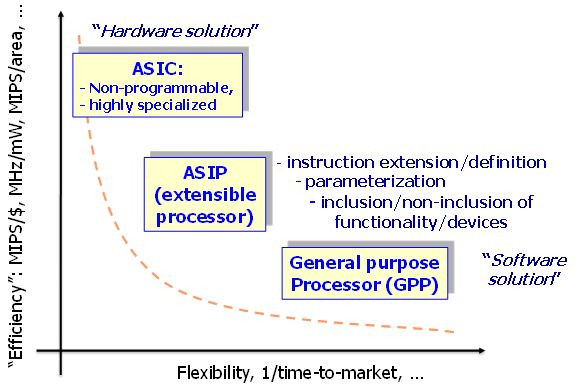
\includegraphics[width=5.86597in,height=4.73125in]{1-1.png}
Figure 1‑1\protect\hypertarget{Fig11}{}{} GPPs, ASIPs and ASICs
{[}Henkel06{]}

ASIPs represent a good trade-off between Application Specific Integrated
Circuits (ASICs) and General Purpose Processors (GPPs), as shown in
Figure \protect\hyperlink{Fig11}{1-1}. ASICs have the highest efficiency
due to the fact, that they are often manually optimized for a specific
task and therefore only the necessary elements are included. This has a
high impact to the power consumption and the execution speed, but it
causes a high time-to-market and high development costs. Nevertheless,
these development costs can amortize when selling a huge amount of
units, due to the lower costs per unit. The GPPs are less efficient due
to the fact, that they are usable for many different kinds of
applications and therefore often contain blocks that are not needed for
a certain task. Whenever an application domain changes frequently due to
e.g. changing standards, then the GPPs are capable to adapt to these
changes, whereas the ASIC would need to be redesigned.

\hypertarget{asip-design-flow}{%
\subsection{ASIP Design Flow}\label{asip-design-flow}}

Designing an ASIP typically starts with analyzing and profiling the
targeted application or application domain, as shown in
\protect\hyperlink{Fig12}{Figure 1-2}. After this analysis, an ASIP is
defined by e.g. specifying its instructions set, embedding blocks that
are required to implement the instructions, and further configuring the
architecture. Traditionally, the step of defining the ASIP is done
manually. However, recent research activities have focused on automating
this process within the range of a manually defined search space.

After the ASIP is defined, a synthesizable hardware description (for
implementing the ASIP) and a tool chain (e.g. compiler, simulator, etc.)
are created automatically. Using these tools and the hardware
description, the ASIP is simulated and benchmarked. This might lead to a
refinement of the ASIP to further optimize it or to keep the
constraints, e.g. the area- or power budget. After the ASIP fulfills the
requirements, a prototype (e.g. FPGA-based) is created and finally, the
ASIP is taped out.
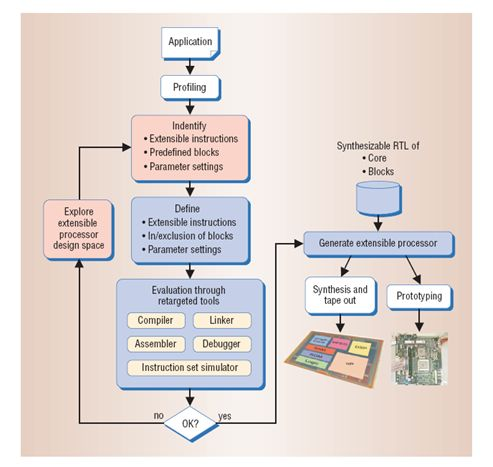
\includegraphics[width=5.86597in,height=4.73125in]{1-2.png}
Figure 1‑2: Typical ASIP Design Flow {[}Henkel03{]}

\hypertarget{custom-instruction-identification}{%
\subsection{Custom Instruction
Identification}\label{custom-instruction-identification}}

Custom Instructions often combine often-executed functionality in one
dedicated assembler instruction. That allows executing this
functionality faster and/or more efficient, etc. Generally, there are
two ways to improve the performance by using Custom Instructions:

\begin{itemize}
\item
  Parallelism: Execute multiple operations that are (data-wise)
  independent from each other in parallel (i.e. at the same time)
\item
  Chaining: Execute multiple operations that are (data-wise) dependent
  from each other sequentially (i.e. after each other) but within the
  same cycle. This might affect the frequency of the ASIP (to assure
  that all operations complete in the same cycle).
\end{itemize}

Both, parallelism and chaining can be applied together in the same
Custom Instruction. Furthermore, sometimes it may also be beneficial to
consider a very different implementation (compared to the given software
implementation of the application) that results in the same
functionality. For instance, to exchange two Bytes within the same Word,
a software implementation has to use \emph{and}, \emph{shift}, and
\emph{or} operations. However, in hardware this corresponds to a simple
re-wiring without any computation and thus can be implemented very
efficient.

There are some constraints for defining Custom Instructions. A Custom
Instruction is typically an unbreakable operation, i.e. it is executed
either completely or not at all. Therefore, the same property has to
hold for the part of the application that is considered to become a
Custom Instruction. An application consist of a certain control flow and
a data flow. The control flow is realized by jumps, loops, etc. The data
flow instead corresponds to the input- and output dependencies of the
operations. An application can be represented as a so-called Base-Block
graph. A Base Block thereby represents a set of operations that are
always executed together (more formally: a sequence of operations that
does not contain a \emph{jump} except at its end and where no
\emph{jump} may enter the sequence except at its beginning). A Base
Block fulfills the above-mentioned requirements of an unbreakable
operation and therefore is a good candidate for a Custom Instruction.
However, sometimes it is possible to embed control flow within a Custom
Instruction. For instance in the case of a MAX operation (i.e.
determining the maximum of two values and assigning it to a result
variable), both control-flow parts (the \emph{then} and the \emph{else}
part) can be embedded inside the Custom Instruction.

There are further constraints that are important when identifying Custom
Instruction. They will be explained by using the example shown in
\protect\hyperlink{Fig13}{Figure~1-3}. Part a) shows a given data flow
within a Base Block (i.e. no further control flow limits the selection
of a Custom Instruction) that is executed very frequently in an
application (and thus is an interesting candidate for a Custom
Instruction). Each node in this graph corresponds to a certain operation
(e.g., addition) and the edges correspond to data dependencies. The
first approach is to try to implement the whole data flow as one rather
larger Custom Instruction. If the critical path of this data flow is too
long (and thus would affect the frequency of the ASIP) the data flow can
be implemented as a so-called multi-cycle operation, i.e. it may require
multiple cycles to execute this instruction (the CPU pipeline is then
typically stalled until the execution completes).

One typical constraint for a Custom Instruction is the amount of
inputs/outputs that are read from/written to the register file. If we
assume that our ASIP provides four read ports and two write ports then
the shown Custom Instruction exceeds these limits. Therefore, we exclude
some nodes of the data flow in part b) of the figure to fulfill the
input/output requirements. Furthermore, there might be so-called
forbidden nodes, i.e. nodes in the data flow that may not be part of a
Custom Instruction. In our example, we have a \emph{load} node, i.e. an
access to the data memory. If we assume that our instruction executes in
the EXE stage of a simple processor pipeline then it might be
complicated to access the resources of the MEM stage to provide access
to the data memory. Therefore, load/store nodes might be forbidden
within a Custom Instruction. In part c) we therefore exclude the
\emph{load} node. However, our Custom Instruction would then no longer
be convex, i.e. we have an edge leaving our Custom Instruction towards a
sub graph (the single \emph{load} node in our example) and another edge
coming from this sub graph and entering our Custom Instruction.
Therefore, our Custom Instruction has to be executed {before} the sub
graph (to provide its input) and {after} the sub graph (to receive its
output) which is obviously not possible at the same time.
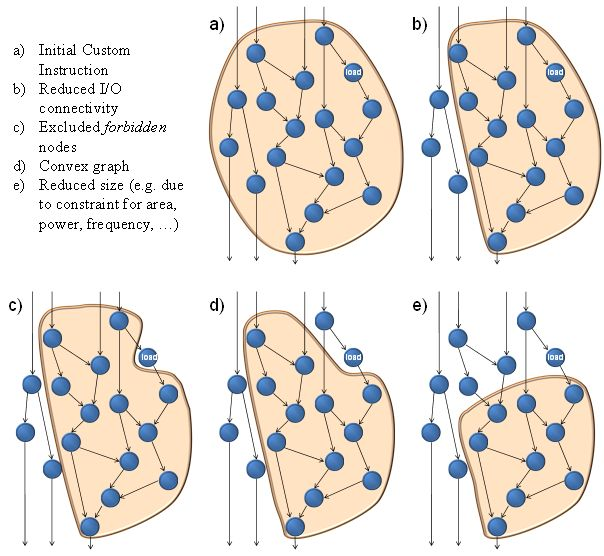
\includegraphics[width=5.86597in,height=4.73125in]{1-3.png}
Figure 1‑3:\protect\hypertarget{Fig13}{}{} Constraints for \emph{valid}
Custom Instructions

To establish the property of a convex Custom Instruction we exclude
further nodes and reach part d) of
\protect\hyperlink{Fig13}{Figure~1-3}. This Custom Instruction now is
convex, does not contain \emph{forbidden} nodes, and respects the
maximal input/output ports of the register file. Therefore, it is a
\emph{valid} Custom Instruction. Further constraints (e.g. the maximum
area, power consumption, or latency) might lead to a further reduction
of the data flow graph, as shown in part e).

\hypertarget{goal-of-the-laboratory}{%
\subsection{Goal of the Laboratory}\label{goal-of-the-laboratory}}

This laboratory will teach the creation of ASIPs from the design, over
the high-level simulation to the final prototype on FPGA hardware.
Benchmarks of speed, needed area and power/energy consumption will be
performed and compared among different created ASIPs. For this purpose
the usage of the different tools have to be practiced and the connection
of these tools to form a tool chain has to be understood. The main goal
is creating new ASIPs for special applications, to benchmark these ASIPs
to find out their benefits and drawbacks and finally to interpret the
benchmark results.

\end{document}
 
\hypertarget{working-environment}{%
\chapter{Working Environment}\label{working-environment}}
This chapter explains the technical environment for the laboratory. This
includes the usage of the computers and the directory structure for this
laboratory. It is very important to understand completely the directory
structure, as many scripts rely on this special structure and will not
work at all or create an unexpected output if the directory structure is
set up in a wrong way.
\hypertarget{network-structure}{%
\section{Network Structure}\label{network-structure}}
The programs needed to perform the laboratory tasks run under Linux. You
will work with the computers in the lab 308.2. This room has 10
computers with Ubuntu 14.04, 32bit installed and are named as follow:
\begin{lstlisting}
i80labpcXX.ira.uka.de where XX=01, 02, \ldots{} 10.
\end{lstlisting}
These computers can also be accessed remotely via SSH or via X2Go
Client, see \protect\hyperlink{remote-operation}{Chapter 2.2.1} and
\protect\hyperlink{x2go-client}{2.2.2}. The user name like asipXX where
XX=01, 02\ldots, 10 and password to login to these computers for
different student groups will be distributed at the beginning of the
lab. You can also access these computers from student lab (Room 312.4)
or from your personal Laptop. X2Go Client is already installed on all
computers in the student lab (Room 312.4) while you have to install and
configure X2Go Client on your Laptop at your own. It is recommended to
use SSH instead of X2Go as it has some conflicts with some settings.

For ASIPmeister and GCC compiler, it is necessary to change the machine
in order to meet the software requirements. There is one dedicated
application workstations:
\begin{lstlisting}
i80pc57.ira.uka.de -- ASIPmeister system:
\end{lstlisting}
You will use this PC for building your own customized CPU and compiler
that is able to use the instructions you added to the instruction set of
the basic processor. This task also needs a powerful machine to complete
in a reasonable amount of time.

To run, this lab, you need to export the following variables, or you can
add it the your /home/.bashrc.user.
\begin{lstlisting}
export ASIPS_LICENSE=29000@i80asip.ira.uka.de
export PATH=/AM/ASIPmeister/bin:$PATH
export ASIP_APDEV_SRCROOT=~/AM_tools
export PATH=/usr/java/jre1.6.0_45/bin:$PATH
export ASIPmeister_Home=/AM/ASIPmeister
export ASIPmeister_HOME=/AM/ASIPmeister
source /home/adm/modelsim_66d.setup
source /home/adm/xilinx_13.2_32bit.setup
\end{lstlisting}
In most cases, you have to manually login into this machine to work with
the ASIPmeister and GCC Compiler. We will provide you the scripts that
will do most of the work for you. Just be aware of the fact that it will
sometimes take time to complete everything. If some errors occur, try to
find out what is wrong by reading the script output carefully. This will
show what went wrong. Start again and if it fails again then ask your
tutor. The most important thing is to know or to recognize that the
results of the script task are right or wrong. This depends on the
output, so read it carefully before starting the next task.

The lab program directory is mounted via NFS to your client. Thus,
almost every program will work on your local machine. Data supplied to
the groups or created by them will be stored on a server directory that
is always available for a client machine. All client machines are
configured as NFS clients, which mount the corresponding home directory
via NFS. This means you can work wherever you want. The hostname will
change, but your home directory will show the same content on all
clients.

To switch between the machines mentioned above you have to use SSH
(recommended). The names of the client PCs are similar to
i80labpcXX.ira.uka.de with the `XX' replaced by the individual number of
the PC. Login with SSH requires authentication, which can be done with
passwords or public keys (see
\protect\hyperlink{remote-operation}{Chapter 2.2.1}). In order to
minimize the efforts for changing machines we recommend public keys, so
you do not have to type your password for every remote login.

\hypertarget{basic-unix-commandsprograms}{%
\section{Basic UNIX
Commands/Programs}\label{basic-unix-commandsprograms}}

If you are familiar with the Unix/Linux environment, you can skip this
section. In this section, ``Unix'' will refer to GNU/Linux mostly.

\begin{itemize}
\item
  \textbf{Command Line Interpreter}: Interaction with the system usually
  is done via the command line, although some file system operation can
  be done with graphical or text based file managers.

The command line interpreter (generally called ``shell'') runs on a
terminal and primarily provides the user with the means to start
programs. It also has several built in commands as well as a scripting
language. The default shell in the lab is \emph{bash} (Bourne Again
Shell).

Some programs and commands require command line arguments (parameters),
which can be supplied in a space-separated list to the program, i.e.:

\emph{cp file1 file2} executes the program ``\emph{cp}'' with the
arguments ``\emph{file1}'' and ``\emph{file2}''.

\item
  \textbf{Online Help System}: Most UNIX commands come with
  documentation in the manual page format (\emph{man}-pages). They
  usually give a detailed description of the program, all command line
  parameters, and some examples. Use the \emph{man} command to read
  \emph{man}-pages, i.e.: ``\emph{man ls}'' calls the \emph{man}-page
  for the ``\emph{ls}'' command. Use the up and down arrow keys (or Page
  Up/Down) to navigate in the man page viewer and ``\emph{q}'' to quit.
\item
  \textbf{Interacting with the File System}
  \begin{enumerate}
  \item
    \textbf{File System Structure}: UNIX organizes all files (regular
    and special files) in a tree structure. The root of the tree is
    called ``/'', directories are the nodes (leaf or non-leaf) and files
    the leaf nodes of the tree. The file system does not have a concept
    of drives -- new data from external media (networked or removable)
    is accessed by attaching the sub tree of the new file system to the
    UNIX file system tree somewhere. Usually ordinary users are not
    permitted to do this.
  \item
    \textbf{Working Directory}: Every process has a current working
    directory -- a pointer to a directory node in the file system tree.
    The current working directory is referred to as ``.'' and the parent
    directory as ``..''. To print the current working directory of the
    shell, use the command ``\emph{pwd}'' (print working directory).
  \item
    \textbf{Home Directory}: Every user has a home directory -- one for
    which he has write access. All your data will be saved in
    subdirectories of your home directory. Home directories are mounted
    via NFS from a remote server. Home directories have the form of
    ``\emph{/home/asip01''} but a user can refer to his home directory
    with ``\emph{\textasciitilde{}}''. Hence,
    ``\emph{/home/asip01/test}'' and ``\emph{\textasciitilde/test''}
    (executed by the user ``\emph{asip01}'') refer to the same.
  \item
    \textbf{File Paths}: To specify a file or a directory, a path name
    must be provided. There are two kinds of paths: absolute and
    relative. An absolute path starts at the root directory, a relative
    path starts at the current working directory. File system nodes
    (path name components) are separated by ``/'' (the same as the
    backslash in Windows). A relative path may be like
    ``\emph{./ASIPMeisterProjects/browstd32}'' which refers to the file
    or directory ``\emph{browstd32}'' of the subdirectory
    ASIPMeisterProjects of the current working directory. An example for
    an absolute path for the same relative path is
    ``\emph{/home/asip01/ASIPMeisterProjects/browstd32}''.
  \item
    \textbf{Changing the Current Working Directory}: To change the
    current working directory use the \emph{cd} command with a path name
    as the argument, i.e.:
\begin{lstlisting}
cd /home/asip01
cd ..
cd ../asip02/ASIPMeisterProjects
cd ./browstd32/Applications
\end{lstlisting}
\item
  \textbf{Creating/Removing Directories}: the ``\emph{mkdir}'' command
  takes a pathname as an argument and creates a new directory accessible
  via this path. The ``\emph{-p}'' parameter tells mkdir to create any
  missing subdirectories as well. ``\emph{rmdir}'' deletes empty
  directories. To remove non-empty directories use the ``\emph{rm}''
  command with the ``\emph{‑r}'' option (see below). Some of the
  examples are:
\begin{lstlisting}
mkdir ~/ASIPMeisterProjects/browstd32/Applications
rmdir ../browstd32/test1
mkdir -p ~/some/non_existing/directory
\end{lstlisting}
\item
  \textbf{Listing Directory Contents}: To examine directory contents use
  the ``\emph{ls}'' command. Without parameters, it will show the file
  and directory names of the current working directory. The
  ``\emph{ls}'' command has many parameters, all described in the
  man-page. Typical ones are ``\emph{‑l}'' to provide a detailed
  listing, ``\emph{‑a}'' to show hidden files (filenames starting with a
  ``.''), ``\emph{‑ltc}'' gives a detailed listing with the last file
  modification time and sort by it (actually these are three
  parameters). Some of the examples are:
\begin{lstlisting}
ls
ls -l ../ASIPMeisterProjects
ls -ltc ASIPMeisterProjects/browstd32/ModelSim
\end{lstlisting}
\item
  \textbf{Moving and Removing Files}: To move or rename a file use the
  ``\emph{mv}'' command with the filename or directory as the argument.
  To remove a file use ``\emph{rm''}; the ``\emph{‑r}'' option causes
  recursive removal of subdirectories and their contents. Some of the
  examples are:
\begin{lstlisting}
mv Applications/tset Applications/test
rm /home/asip01/oldfile
rm -r ../browstd32
\end{lstlisting}
\item
  \textbf{Copying Files}: The ``\emph{cp}'' command copies files and
  directories. Its arguments are: optional switches, then the source and
  the target file/directory respectively. The ``\emph{‑r}'' switch
  enables recursive copying. Some of the examples are:
\begin{lstlisting}
cp TestData.IM TestData.IM-backup
cp -r browstd32 browstd32\_custom
\end{lstlisting}
\end{enumerate}
\item \textbf{Shell Operation:}

  \begin{enumerate}
  \item
    \textbf{Input/Output Redirection}: Some programs read data on their
    standard input file descriptor (stdin), some write output to the
    standard output (stdout). Usually stdin is linked to the keyboard
    and stdout to the terminal screen. However, you can change this when
    calling a program. ``\emph{\textless{} somefile}'' redirects stdin
    to read from ``\emph{somefile}'' and not from keyboard, likewise
    \emph{``\textgreater{} someotherfile}'' will redirect stdout to
    write to ``\emph{someotherfile}'' (if it doesn't exist, it will be
    created, if it does, it will be truncated first -- use
    ``\emph{\textgreater\textgreater{} someotherfile}'' to append
    instead of truncating the previous contents. Redirection is also
    possible to/from other processes via pipes: use ``\emph{program1
    \textbar{} program2}'' to direct the output of ``\emph{program1}''
    to the input of ``\emph{program2}''. Some of the examples are:
\begin{lstlisting}
ls -ltc >filelisting
ls | sort
cat <file1 >>file2 (this appends the contents of file1 to file2).
\end{lstlisting}
\item \textbf{Job Control}: Processes started from the shell are often
  referred to as ``\emph{jobs}''. Usually, when the shell launches a
  program it will take control of the terminal and the shell will be
  suspended until the process terminates -- the job ``is running in the
  foreground''. To launch a job ``in the background'' -- start it, but
  give control back to the shell immediately, append ``\&'' at the end
  of parameter list. To list any jobs launched from this shell (they all
  have to be in the background), type ``\emph{jobs}'' -- this will give
  you the job-IDs with the program names and parameters of the jobs. To
  bring a job to the foreground, use ``\emph{fg \%job-ID}'' (substitute
  job-ID for the actual job ID). Sometimes you will want to temporarily
  stop a job -- if the program is in the foreground, hit ``CTRL-Z'' (job
  suspension). To continue job execution in the foreground use
  ``\emph{fg}'' as described above, or ``\emph{bg \%job-ID}'' to
  continue execution in the background.
\end{enumerate}

To terminate a job in the foreground, hit ``CTRL-C'' (send keyboard
interrupt). Note that if a process is unresponsive (due to bugs -- i.e.
endless loop and signal processing disabled) it can ignore this; the
only way to terminate it is to send a KILL signal as explained below).
\item
  Some important programs and commands
  \begin{enumerate}
  \item
    \textbf{Process/Activity Listing}. To view a complete list of
    running processes, use the ``\emph{ps}'' program. It is mostly used
    with the ``\emph{auxw}'' options to provide a complete and detailed
    listing. The output is usually quite long, so it is often piped into
    ``\emph{less}'' or ``\emph{head}''.
  \item
    \textbf{Text Viewer}. ``\emph{less}'' is a program to view text (you
    can use it to view binary data as well, but it treats it as a byte
    stream without any special formatting, except for control characters
    -- they are substituted). The argument is the file to view;
    otherwise, data can be piped if used without any arguments. To
    scroll through the ``\emph{less}'' output use the up and down arrow
    keys (or Page Up/Down) to navigate, ``\emph{q}'' to quit. To jump to
    a specific line (current line and byte numbers are displayed at the
    bottom), type the line number followed by \emph{G} (i.e. \emph{123G}
    to jump to line 123). Some of the examples are:
\begin{lstlisting}
less ModelSim/TestData.DM
ps axuw | less
\end{lstlisting}
\item
  \textbf{Difference between Files}: The ``\emph{diff}'' program
  examines two files for differences and displays these. Useful to
  compare outputs of programs and see if and what changes occurred.
  Common options are ``\emph{‑u}'' (unified output) to have verbose
  output. Unified output lists the lines that were in the old file, but
  are not in the new file preceded with a ``-`` and files that were not
  in the old file and are in the new file preceded with a ``+''. Lines
  that start with neither are just context to make orientation a bit
  easier. File sections where changes were detected start with @@,
  followed by the line ranges of the sections. A graphical diff-tool
  that visualizes the output of ``\emph{diff}'' is ``\emph{kompare}''
  (the `k' instead of `c' for `compare' denotes that it is meant for
  kde; so this is not a typing error). Some of the examples are:
\begin{lstlisting}
diff -u TestData.DM-OLD TestData.DM | less
kompare EvilFile.txt GoodFile.txt &
\end{lstlisting}
\item
  \textbf{Show only the Beginning/End of a File/Output}. The
  ``\emph{head}'' and ``\emph{tail}'' programs show only the first and
  last lines (respectively) of a file or the data that are piped in. By
  default they show 10 lines, but the ``\emph{‑n x}'' option sets it to
  x lines. Tail can also monitor a file for future appends and display
  them (useful when watching log files of a running program). This is
  requested with the ``\emph{‑f}'' option. Some of the examples are:
\begin{lstlisting}
ls -ltc Applications/bubblesort | head -n 5
tail -n 0 -f /tmp/logfile
\end{lstlisting}
\item
  \textbf{Show Machine's Activity Summary}: while the ``\emph{ps}''
  command gives a detailed overview of the running processes, sometimes
  a summary is more useful. ``\emph{top}'' shows the current number of
  running processes, the CPU(s), memory and swap usage and the active
  processes. It updates every three seconds and can be exited with
  ``\emph{q}''.
\end{enumerate}
\end{itemize}
\hypertarget{remote-operation}{%
\subsection{Remote Operation}\label{remote-operation}}
\begin{enumerate}
\item
  \textbf{Remote login}. To log onto a different machine, the SSH
  program is available (Secure Shell). Communication between the two
  machines is encrypted by SSH. To simply log onto a different machine
  with the current user, use ``\emph{ssh~hostname}''. If your account
  username is not the same as on the local machine use
  ``\emph{ssh~otheruser@hostname}'', where ``\emph{otheruser}'' is the
  username of the account on the remote machine. SSH will ask for a
  password on the remote machine, and then log in and start a shell.
  ``\emph{exit}'' will end the remote shell and terminate the SSH
  connection leaving you on your local machine.
\item
  \textbf{Copying via SSH}: Not all machines have NFS mounted home
  directories, so you will sometimes have to copy files to a remote
  machine. The SSH package provides ``\emph{scp}'' for this, which can
  copy files or directories from one machine to another (if you have an
  account on the remote machine). The syntax is ``\emph{scp somefile
  remotehost:}'' (note the colon at the end, omitting it will cause scp
  to copy ``somefile'' to the file ``remotehost'' on the local machine).
  To copy directory trees use ``\emph{scp -r directory remotehost:}''
\item
  \textbf{X11 Forwarding}: GUI programs can be run on remote machines as
  well. Log in on a remote machine with ``\emph{ssh -X remotehost}'' and
  start a program installed on remotehost. It will be displayed on your
  machine, but will run (access files and use resources -- CPU, memory,
  etc.) on remotehost.
\item
  \textbf{Public Key Authentication}. An alternative to providing
  passwords for every login is public key authentication mode. A key
  pair is created on your local machine and you can copy the public key
  to any machine you want to log on later. Once set up, authentication
  is done automatically and no interactive passwords are necessary. The
  steps to setup a public key authentication is as follows:

  \begin{enumerate}
  \def\labelenumii{\roman{enumii}.}
  \item
    First, create the DSA-keys by logging into any machine and invoking:
\begin{lstlisting}
ssh-keygen --t dsa
\end{lstlisting}
Confirm the default destination for the keys. Afterwards enter your pass
phrase, for example, your group name or you can just leave it empty.
Sometimes you will be asked for this, so remember what you entered.
Public and private keys will be stored in your
``\emph{\textasciitilde/.ssh}'' directory.
\item
  Then copy the public key to the remote machine:
\begin{lstlisting}
ssh-copy-id --i \textasciitilde/.ssh/id\_dsa.pub user@remote-machine
\end{lstlisting}
\end{enumerate}
\end{enumerate}
Enter your password to confirm this step. Afterwards log out and try to
log in again. This should work without asking you to enter the password.

\hypertarget{x2go-client}{%
\subsection{X2Go Client}\label{x2go-client}}

X2Go is a program used to run graphical applications on Linux machines
remotely. This uses a technology, which results in better performance.
This also allows for suspending and resuming sessions and programs,
while they are running. This allows the use of long-running graphical
applications.

\begin{itemize}
\item
  Installation
  \begin{enumerate}
  \def\labelenumi{\alph{enumi}.}
  \item
    The X2Go Client software is already installed on all computers in
    out student lab.
  \item
    For your Laptop, you can download and install the X2Go Client from:
    \url{http://wiki.x2go.org/doku.php/download:start}
  \end{enumerate}
\item
  Configuration

When you first run the X2Go client, a "\emph{New session}" dialog should
appear otherwise you can create new session using ``\emph{Session}''
menu and then clicking on ``\emph{New Session\ldots{}}'' You should fill
this in with the following information in ``\emph{Session}'' tab:
\begin{enumerate}
\def\labelenumi{\alph{enumi}.}
\item
  Session name - Any name you like to identify the session - if you're
  connecting to the PC ``\emph{i80labpc01}'', you might just want this
  to be " \emph{i80labpc01}"
\item
  Host - Full name of the computer you're connecting to, e.g.
  ``\emph{i80labpc01.ira.uka.de}''
\item
  Login - Your user ID, for example ``\emph{asip01}''
\item
  Session type - Select XFCE (recommended) - This is a low-power window
  manager that is the only one supported in the current version of
  Ubuntu.
\item
  Keep all the other setting to default.
\end{enumerate}
\item
  Connecting
  \begin{enumerate}
  \def\labelenumi{\alph{enumi}.}
  \item
    To start the session, click on it and enter your password when
    prompted
  \item
    After you click OK, it will connect to the server and start your
    session. Watch the Status line to see what is happening. Once the
    status is "running," your session should launch.
  \item
    Sometimes "\emph{i80labpcXX}" cannot be accessed remotely using
    X2Go, while it works fine with SSH. May be there is a conflict
    between some settings in your \textasciitilde/.bashrc.user and X2Go.
    For example one temporary solution is to comment out the line ".
    /home/adm/xilinx\_13.2\_32bit.setup" in
    \textasciitilde/.bashrc.user. This makes X2Go work properly. If
    Xilinx ISE is required, you can source it manually.
  \end{enumerate}
\end{itemize}
\hypertarget{directory-structure}{%
\section{Directory Structure}\label{directory-structure}}
In development environments it is very useful to force developers to
meet certain rules how program data is stored. Therefore, we provide a
template that makes it easier for the tutors to find the results of
every group and enables us to write script files that work on fixed
locations to speed up the work. On the other hand, these script depend
on this directory structure. You have to understand and use this
directory structure to avoid problems.

The main directory structure is shown in Figure \ref{fig:fig21}. Your home directory contains one
special directory called ``\emph{ASIPMeisterProjects}''. All your
ASIPMeister Projects including your applications and all other files
will be placed in this directory. Inside this
``\emph{ASIPMeisterProjects}''-directory every project has a
subdirectory (e.g. ``\emph{browstd32}'' or ``\emph{AnotherProject}'').
We recommended that you create new subdirectory/project for each changed
version of the CPU. Among the projects the
``\emph{ASIPMeisterProjects}''-directory also includes a
``\emph{TEMPLATE\_PROJECT}''. This directory gives you a basic ASIP
Meister Project with minimum director structure and files required to
start your ASIP projects. This template is a good starting point to
create a new project from the scratch. Usually you can copy from your
last project to create a new one, but sometimes it is recommended to
start from the scratch.
\begin{figure}[!htb]
	\centering
	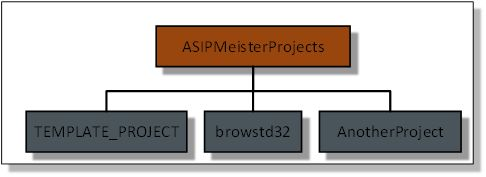
\includegraphics[width=0.9\textwidth]{src/images/2-1.png}
	\caption{ The Directory Structure for all ASIP Meister Projects}
	\label{fig:fig21}
\end{figure}
The biggest part of the directory structure is placed inside each ASIP
Meister project directory, e.g. ``\emph{browstd32}'', as shown in Figure
\ref{fig:fig21}. Every project directory contains
\textbf{five} subdirectories and a set of local files. These directories
and files are explained in the following sections.

The \textbf{``Applications''} directory should contain all your user
applications that you want to run and simulate on the CPU, each in a
separate subdirectory. Every application should be placed inside a
separate subdirectory for this application along with a \emph{Makefile}
that is needed to compile, simulate and implement the application. When
you want to compile an application, simulate it (dlxsim or ModelSim),
generate its bitstream for FPGA, or upload its bitstream into FPGA, you
run the \emph{Makefile} in that particular application subdirectory. To
see different options that \emph{Makefile} offers, execute
``\emph{\textbf{make}}'' in an application subdirectory, as shown below:
\begin{lstlisting}
asip04@i80labpc04:~/ASIPMeisterProjects/browstd32/Applications/Application1:$make
/--------
| USAGE:
\--------
'make sim':    compile for dlxsim/Modelsim
'make dlxsim': compile for dlxsim and directly start simulation
'make fpga':   compile for FPGA and update bitstream
'make upload': upload the existing bitstream to the FPGA (note: this command does not generate a new bitstream)
'make all':    compile for dlxsim/Modelsim and for FPGA
'make clean':  delete the BUILD directories

/---------------------
| PASSING PARAMETERS:
\---------------------
'DLXSIM_PARAM=...'
Example: 'make dlxsim DLXSIM_PARAM="-da0 -pf1"'
Note:    These are the default parameters. Don't forget the double high-commas (i.e.: ") when passing multiple parameters.
'GCC_PARAM =...'
Example: 'make sim GCC_PARAM =-O3'
Example: 'make dlxsim GCC_PARAM =-O3 DLXSIM_PARAM="-da0 -pf1"'
Note:    If you want to enfore re-compilation with different parame-ters then you have to 'make clean' to make sure that all files are re-compiled
\end{lstlisting}
For example, if you want to work with ``\emph{Application1}'', as shown
in Figure \ref{fig:fig23}. Your first step is to compile
this application. Inside the ``\emph{Application1}'' directory
containing source code ``\emph{application1.c}'' or
``\emph{application1.s}''. To compile it you have to execute the
following in the ``\emph{Application 1}'' directory:

asip04@i80labpc04:\textasciitilde/ASIPMeisterProjects/browstd32/Applications/Application1:\$make
sim

The \emph{Makefile} is expected to be executed from the directory, where
the results will be placed, so always execute the scripts from the
application specific subdirectory, never from the
``\emph{Applications}'' directory itself! The details about the
parameters, the created output files and the different versions of the
Makefile scripts are explained in Table \ref{fig:fig22}.
The concept of calling the scripts from the specific application
subdirectory is also important for the Makefile script while executing
``\emph{make sim}'', ``\emph{make dlxsim}'', ``\emph{make fpga}'' and
``\emph{make upload}'' as explained in Table \ref{fig:fig22}.
\begin{table}[!htb]
	\centering
	\begin{tabular}{|l|p{13cm}|}
		\hline
		\multicolumn{1}{|c|}{\textbf{Script}} & \textbf{Description}                                                               \\ \hline
		make sim 
		& It will compile your assembly or C-file file in your current application
		directory and ``\emph{BUILD\_SIM}'' subdirectory is created in your
		current directory containing different files like ``\emph{TestData.IM}''
		and ``\emph{TestData.DM}'' file for the ModelSim. The output assembly
		file named ``NameOfTheApplication-Directory.dlxsim'' will also be
		generated. You can pass different parameters to this Makefile as
		follows:
		\begin{enumerate}
			\item
			\emph{GCC\_PARAM} is used to set optimization level for GCC Compiler.
			The compiler options are directly forwarded to the compiler binary
			e.g. ``-O0'' or ``-O4'' for different optimization levels. for
			example:
		\end{enumerate}
		make sim GCC\_PARAM =-O3\strut \\\hline
		make dlxsim      
		& It will start the dlx simulator to simulate the compiled file generated
		from the previous stage. Similar to previous command,
		``\emph{BUILD\_SIM}'' containing different files like
		``\emph{TestData.IM}'', ``\emph{TestData.DM}'' and
		``NameOfTheApplication-Directory.dlxsim'' is created. Here, you have to
		pass some parameters to dlxsim mentioned in the Figure. You can also
		pass \emph{GCC\_PARAM} with this command. Another parameter that is
		required with this command is DLXSIM\_PARAM, which is used to pass
		different dlxsim parameters, for example:
		
		make dlxsim DLXSIM\_PARAM="-fAppName.s -da0 --pf1 -lfputc.out "
		
		In the command, ``\emph{AppName.s}'' is loaded into dlxsim for
		simulation, without debugging and with pipeline forwarding. Moreover,
		``\emph{putc.out}'' is the file containing the printed output. Executing
		``\emph{make dlxsim}'' without any parameters, will execute the file
		``\emph{BUILD\_SIM/AppName.dlxsim}'' with ``\emph{-da0}'' and
		``\emph{-pf1}''.\strut  \\\hline
		make dlxsim-test        
		& To disrupt, emancipate, transform the habitus and field of design To explore how the user is affected by design practices, objects and systems To change design practices, \\\hline
		make fpga &       
		It will compile your assembly or C-file, generate the
		required DM/IM file, and combine them with your bitstream that is
		generated from the ISE Project. Finally, a new bitstream file containing
		your hardware CPU along with corresponding IM/DM files of your
		application will be generated in the subdirectory ``\emph{BUILD\_SIM}''.
		This bitstream will be used to configure the FPGA. \\ \hline
		make upload &        
		It will upload the existing bitstream to the FPGA
		BlockRAM. Note that this command does not generate a new
		bitstream. \\ \hline
		make clean &       
		It cleans your current project directory by deleting
		``\emph{BUILD\_SIM}''. \\	\hline
		make all &       
		It will compile for dlxsim and for ModelSim and generate
		final bitstream for FPGA. \\	\hline
	\end{tabular}
	\caption{Makefile Options and Parameters}
\label{fig:fig22}
\end{table}
\begin{figure}[!htb]
	\centering
	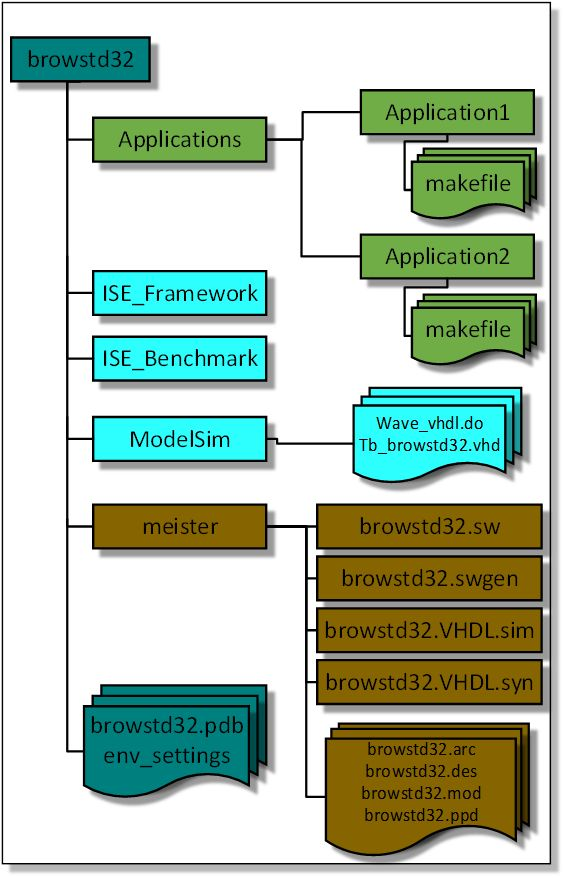
\includegraphics[width=0.8\textwidth]{src/images/2-3.png}
	\caption{The Directory Structure for a Specific ASIP Meister Project}
	\label{fig:fig23}
\end{figure}
The \emph{Makefile} script inside the ``\emph{Applications}'' directory
is only wrapper for the real scripts. This wrapper first read the
``\emph{env\_settings}'' file from your project directory (e.g.
``\emph{browstd32}'' in Figure \ref{fig:fig23}). This
file contains all the information about your current project, e.g. which
compiler to use and which dlxsim to call. Afterwards the wrapper script
calls the real scripts. The real scripts are placed at a global
position. This enables us to make changes to these scripts without the
need to copy these changes to all your projects. The
``\emph{env\_settings}'' file is explained in Table \ref{fig:fig25}.

The \textbf{``\emph{meister}''} directory contains the ASIP Meister
output, like the VHDL and compiler generation files. ASIP Meister
automatically creates this ``\emph{meister}'' directory. This meister
directory is always created at the place, where ASIP Meister is started.
So execute ASIP Meister inside your project directory (\emph{browstd32}
in this example)! It is very important, that you always start ASIP
Meister in your current project directory. Otherwise, the other scripts
will not find the meister subdirectory or even worse: they work with an
old version of the meister directory. The directory ``\emph{meister}''
contains three subdirectories for the simulation VHDL files
(\emph{browstd32.sim}), the synthesis VHDL files (\emph{browstd32.syn})
and the software description (\emph{browstd32.sw}) respectively for the
project ``\emph{browstd32}''. Some additional files are placed inside
the meister directory itself. The most important file here is the
``\emph{browstd32.des}'' file. This file contains all information that
is required to create a binary file out of an assembly file, i.e. to
assemble an assembly file. This file can be automatically extended with
user instructions, as explained in Figure 2‑4:. From the subdirectories,
you will mostly need the VHDL files from ``\emph{browstd32.syn}'' for
simulation in ModelSim as explained in Chapter~5 and for synthesis as
explained in Chapter~6. Inside the ``\emph{browstd32.sw}'' directory,
which is needed for creating the GCC compiler, you will mostly need the
``\emph{instruction\_set.arch}'' file, as explained in Chapter~8.2. This
file contains the summary of all assembly instructions that the compiler
will support, but sometimes this file has to be manually edited before
starting the automatic compiler generation.

The \textbf{``ModelSim''} directory will contain your ModelSim project
for simulating the CPU at VHDL level. ModelSim itself is explained in
Chapter~5. It is important, that you start ModelSim inside this
``\emph{ModelSim}'' directory, as it searches for specific files at the
position where it was started. There are \textbf{five} files already
placed in this directory containing the test bench and some
configuration to monitor some CPU internal signals. The details (e.g.
how to use these files) are explained in Chapter~5.1.

The \textbf{``}\textbf{ISE\_}\textbf{Framework''} directory contains
some predesigned framework files that are required for the connection
between CPU, Memory, UART, and all other components. The framework
consists of three types of file and all of them have to be added to the
ISE project.

\begin{itemize}
\item
  The VHDL files describe how all components are connected together.
\item
  The UCF file describes the user constraints (e.g., which I/O pins
  should be used and which clock frequency is requested).
\item
  The BMM file contains a description of the memory buildup for
  instruction- and data-memory for the CPU. Out of this file
  ``\emph{\ldots\_bd.bmm}'' file will be generated while implementation
  and this file will be used to initialize the created bitstream with
  the application data, as explained in Chapter~6.4.
\item
  \textbf{IP cores} are used within the framework, e.g. memory blocks
  for instruction- and data-memory or FIFOs for the connection to the
  LCD. These IP cores are not available as VHDL source code, but instead
  they are available as pre-synthesized net lists. These files just have
  to be copied into the directory of your ISE project (no need to
  actually ``\emph{add}'' them to the project) and then they will be
  used in the ``\emph{implementation}'' step. The needed *.ngc files are
  available in
  ``\emph{/home/asip00/­ASIPMeisterProjects/­TEMPLATE\_PROJECT/­ISE\_Framework/­IP\_­Cores}''.
  Note: The files {inside} the IP\_Cores directory have to be copied to
  your ISE Project Directory. It is not sufficient to copy the full
  IP\_Cores directory!
\end{itemize}

The \textbf{``ISE\_}\textbf{Benchmark''} directory contains some
predesigned files to benchmark only your CPU more accurately as compared
to ``\emph{ISE\_Framework}''. The ``\emph{ISE\_Benchmark}'' consists of
four files: ``\emph{bram\_dm.ngc}'', ``\emph{brom\_im.ngc}'',
``\emph{dlx\_}\emph{toplevel.vhd}'', and ``\emph{dlx\_ toplevel.ucf}''.
The first two files are BlockRAM netlist files for data and instruction
memories. The VHDL file is the top level for the whole project. The UCF
file specifies the timing constraints and pins location for the design
(in this step, we specify only the clock and reset constraints).

Inside your \textbf{project directory} (``browstd32'' in the example
from Figure \ref{fig:fig23} are some local files that
are explained in Table \ref{fig:fig24}.
\begin{table}[!htb]
	\centering
	\begin{tabular}{|l|p{12cm}|}
		\hline
		\multicolumn{1}{|c|}{\textbf{Filename}} & \textbf{Explanation}                                                               \\ \hline
		browstd32.pdb & The ASIP Meister project file, i.e. your CPU design. If
		you use this filename as parameter when starting ASIP Meister then the
		design will immediately be loaded. It is important that you always start
		ASIP Meister inside your current project directory, as otherwise the
		meister directory will be created at the wrong place, i.e. at a place
		where the scripts don't expect it.
		\\ \hline
		env\_settings & This file contains all settings for your project. Every
		script that you call evaluates this file, so you have to take care that
		the information in this file is correct. After you create a new project
		directory, your first task is to adapt this file. The entries in this
		file will be explained in the Figure 2‑5:. The first 3 settings are the
		most important ones; the other settings will rarely be
		changed.
		\\ \hline
	\end{tabular}
	\caption{The Files in a Project Directory}
	\label{fig:fig24}
\end{table}
The settings and paths for your project directory should be properly
configured in the file ``\textbf{env\_settings}'' as explained in Figure
2‑5:.
\begin{table}[!htb]
	\centering
	\begin{tabular}{|p{6cm}|p{11cm}|}
		\hline
		\multicolumn{1}{|c|}{\textbf{Setting}} & \textbf{Explanation}                                                               \\ \hline
		PROJECT\_NAME = browstd32 & This is the name of your project directory
		(``\emph{browstd32}'' in Figure \ref{fig:fig21} or for
		example ``\emph{AnotherProject}'' in Figure \ref{fig:fig23}). Whenever you create a new project with a new directory, then you
		have to adapt this parameter.
		\\ \hline
		CPU\_NAME = browstd32 & This is the name of the ASIP Meister project
		file (``\emph{browstd32.pdb}'' in Figure \ref{fig:fig23}). As the names of subdirectories inside the ``\emph{meister}''
		directory depend on the name of the ASIP Meister project file. You need
		to change this value, according to the ASIP Meister project name in the
		project directory.
		\\ \hline
		DLXSIM\_DIR = /home/asip00/epp/dlxsim & This is the full path to the
		dlxsim simulator directory, as explained in Chapter~3.3. If you want to
		use a modified version of dlxsim, then you can just copy this directory
		into your home, make your changes and adapt this setting to use your
		modified version.
		\\ \hline
		ISE\_NAME = ISE\_Framework & This is the name for your ISE project where
		you can synthesize your CPU for the hardware platform, as explained in
		Chapter~6. This directory setting is used to combine the synthesis
		result with an application, as explained in Chapter~6.4.
		\\ \hline
		ASIPMEISTER\_PROJECTS\_DIR =
				\textasciitilde/ASIPMeisterProjects & This is the directory name for
		all your ASIP Meister projects, e.g. ``\emph{ASIPMeisterProjects}'' as
		explained in Figure \ref{fig:fig21}.
		\\ \hline
		PROJECT\_DIR = \$\{ASIPMEISTER\_PROJECTS\_DIR\} /\$\{PROJECT\_NAME\} &
		This is the full directory name for your current project. You do not
		need to change this. The only thing you need to do is to change the
		settings for the project name, as mentioned above.
		\\ \hline
		MEISTER\_DIR = \$\{PROJECT\_DIR\}/meister & The full directory name of
		the ``\emph{meister}'' subdirectory. You do not have to change this
		value.
		\\ \hline
		MODELSIM\_DIR = \$\{PROJECT\_DIR\}/ModelSim & The full directory name of
		the ``\emph{ModelSim}'' directory. When compiling an application, as
		explained in Table \ref{fig:fig22}, the created
		``\emph{TestData.DM}'' \& ``\emph{TestData.IM}'' will automatically be
		copied to this directory.
		\\ \hline
		\vtop{\hbox{\strut ISE\_DIR =
				\$\{PROJECT\_}\hbox{\strut DIR\}/\$\{ISE\_NAME \}}} & The full directory
		name of the ISE project. You do not have to change this
		value.
		\\ \hline
		MKIMG\_DIR = /home/asip00/epp/mkimg & The full directory name for the
		different ``\emph{Makefile}'' scripts, as explained in
		Table \ref{fig:fig22}. Usually, you do not have to
		change this value.
		\\ \hline
		COMPILER\_NAME = brownie32-elf-gcc & The name of the compiler
		binary.
		\\ \hline
		ASSEMBLER\_NAME = brownie32-elf-as & The name of the assembler
		binary.
		\\ \hline
		LINKER\_NAME = brownie32-elf-ld & The name of the linker
		binary.
		\\ \hline
		COMPILER\_DIR = \$\{MEISTER\_DIR\}/ \{CPU\_NAME\}.swgen/bin & The full
		directory name for the customized compiler for customized CPU, which is
		located in the ``meister'' directory in the current
		project.
		\\ \hline
		PATH=\$\{MEISTER\_DIR\}/\$ \{CPU\_NAME\}.swgen/bin:\$PATH & Add the
		compiler binary location in the PATH environmental
		variable.
		\\ \hline
	\end{tabular}
	\caption{The Configurable Settings for an ASIP Meister Project}
	\label{fig:fig25}
\end{table}
 
\hypertarget{dlxsim}{%
\chapter{Dlxsim}\label{dlxsim}}

Dlxsim \cite{DLX-Package}-\cite{DLXsim} is an instruction accurate simulator for DLX
assembly code \cite{Hennessy96}-\cite{Sailer96}. In this laboratory, we will use a modified version of
dlxsim, which is changed in such a way, that it is behaving like the
ASIP Meister specific implementation of the Brownie STD 32 Processor,
which will be created and used in the later steps of the laboratory. In
the first subchapter, some basic ideas about the Brownie architecture
and the Brownie instruction set will be introduced. Afterwards the basic
usage of dlxsim will be explained. In the last subchapter, it is shown
how dlxsim can be extended to support new assembly instructions, which
will be added to the Brownie processor with ASIP Meister.

\hypertarget{brownie-std-32-architecture}{%
\section{Brownie STD 32
Architecture}\label{brownie-std-32-architecture}}
Brownie STD 32 (browstd32.pdb) is a RISC-type pipeline processor
architecture. The Brownie architecture is designed for an easy and fast
\textbf{pipeline processor}. It is a \textbf{Load-/Store-architecture},
which means that there are dedicated commands for accessing the memory
and that all the other commands only work on registers, but not on
memory addresses. As an implication, the Brownie architecture has a
\textbf{big uniform register file} that consists of 32 registers with 32
bits each, where some registers are special registers like the register
r0 has a special meaning, as it is hard wired to zero. The pipeline
stages for the Brownie processor are the following:

\begin{enumerate}
\def\labelenumi{\arabic{enumi}.}
\item
  Instruction Fetch (\textbf{IF}): This phase reads the command on which
  the program counter (PC) points from the instruction memory into the
  instruction register (IR) and increases the PC.
\item
  Instruction Decode (\textbf{ID}): Here the instruction format is
  determined and the respectively needed parameters are prepared; e.g.
  reading a register from the register file or sign extending an
  immediate value.
\item
  Execute (\textbf{EXE}): The specific operation is executed in this
  phase for the parameters, which have been prepared in the preceding
  stage.
\item
  Memory Access and Write Back (\textbf{WB}): If the command is a memory
  access, then the access will be executed in this phase. Every
  non-memory access command will pass this stage without any activity.
  Finally, the result that has been computed or loaded will be written
  back to the register file.

  The memory architecture of Brownie STD is Harvard. Both of the
  instruction length and the data length are 32 bit. Addressing can be
  performed in byte. Brownie has 32 integer general-purpose registers
  and a 4-stage pipeline structure, each stage of which is named IF, ID,
  EXE and WB. Full forwarding to the pipeline makes the operation
  results of all the instructions immediately usable. Brownie STD
  executes delayed load for load type instruction, and the number of
  delayed slot is one. Brownie STD does not have a delayed branch slot
  (does not execute delayed branch). Brownie STD does not have a
  floating-unit operation. A floating-point execution instruction can be
  added as a custom instruction. Basic architecture parameters are shown
  in the following table.

  In Figure \ref{fig:fig32}, an example for some
  overlapping commands in a 5-stage pipeline (DLX processor) is shown.
  In the first command, the values from the registers \emph{r2} and
  \emph{r3} are added and the result is stored in register \emph{r1}.
  The write back to \emph{r1} is done in clock cycle 4, so it cannot be
  read earlier than in clock cycle 5. The last command of the shown
  pipeline example is using \emph{r1} as input and it is scheduled in
  such a way, that it is reading \emph{r1} in clock cycle 5, so that it
  is using the latest value that has just been written back by the first
  command. \emph{The example shows, that three successive NOPs are
  enough to resolve a data dependency.} The Brownie processor is using a
  \textbf{data forwarding} technique to resolve such data dependencies
  without the in-between NOPs, and ASIP Meister does support full
  forwarding i.e. data and branch forwarding is available in this
  version of ASIPmeister. Therefore, for ASIP Meister generated
  processors, the NOPs are not needed to resolve the data dependencies
  (as shown in Chapter~3.2.1 you can configure dlxsim to behave in both
  ways, i.e. with or without data forwarding).
\end{enumerate}
\begin{longtable}[!htb]{@{}ll@{}}
\toprule
\textbf{Parameters} & \textbf{Architecture}\tabularnewline
\midrule
\endhead
Basic architecture & RISC\tabularnewline
Memory architecture & Harvard\tabularnewline
Instruction length & 32\tabularnewline
Data length & 32\tabularnewline
Addressing & Byte address\tabularnewline
The number of general-purpose registers & 32\tabularnewline
The number of pipeline stages & 4\tabularnewline
The number of delayed branch slot & 0\tabularnewline
Floating-point unit & N/A\tabularnewline
Forwarding & full forwarding\tabularnewline
Alignment & 1-byte, 2-byte and 4-byte\tabularnewline
Endian-ness & Big Endian\tabularnewline
Interrupts & Reset, Internal, External\tabularnewline
\bottomrule
\caption{Brownie STD 32 Architecture Parameters}
\label{fig:fig31}
\end{longtable}
The \textbf{instruction set} of the BROWSTD32 architecture is separated
into four \textbf{instruction classes} (arithmetic for integer,
arithmetic for float, load/store and branch), which are implemented in
different \textbf{instruction formats}, as shown in Figure \ref{fig:fig33}. The arithmetic instructions use
either an instruction format for three registers or an instruction
format for two registers and an immediate value. The load/store
instructions always use the format with two registers and one immediate,
where the effective address is computed as the sum of one register (as
base address) and the immediate value. The other register is used either
as value to store in memory or as register where to place the loaded
value. The branch instructions are divided into conditional branches and
unconditional jumps. The jumps use an instruction format with a 26-bit
immediate value as a PC-relative jump-target. The \emph{jump register}
instructions instead use the I-Format to declare in which register the
absolute jump target is placed. The second register and the immediate
value are not used by these instructions. The conditional branches need
a field for a register that contains the condition, so they use the
I-Format as well. They use the 16-bit immediate as PC relative jump
target. The second available register is not used.
\begin{figure}[!htb]
	\centering
	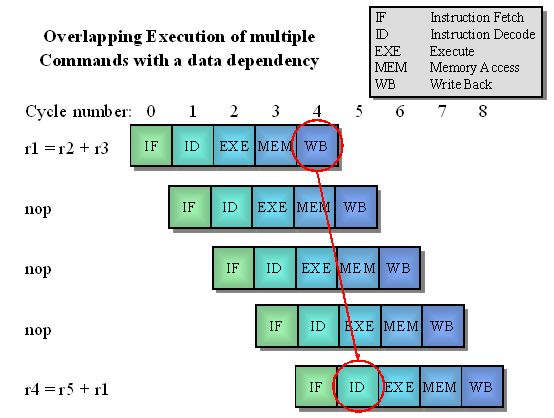
\includegraphics[width=0.9\textwidth]{src/images/3-2.png}
	\caption{BROWSTD32 Pipeline Example with a Data Dependency}
	\label{fig:fig32}
\end{figure}
For many assembly-commands, there are special versions for dealing with
unsigned values and for using immediate values as second input
parameters. These versions have an attached ``i'' for ``immediate''
and/or an attached ``u'' for ``unsigned'' as suffix (e.g. addui). A
summary of all assembly instructions that are available in the ASIP
Meister specific implementation of the BROWSTD32 processor that is used
in the laboratory (i.e. browstd32) is shown in Figure 3‑4:. For a more
detailed description of the assembly-commands have a look into \cite{Sailer96}.

Finally, some specialties in the architecture need to be mentioned:
\begin{itemize}
\item
  \textbf{Delay slots:} Without forwarding, an instruction, that is
  placed right after an unconditional jump or a conditional branch
  instruction is always executed. In fact, there are two instructions,
  that enter the pipeline, but only the first one is executed, the
  second one will not be allowed to write the computed result back to
  the register file. But, in Brownie this is handled automatically using
  full-forwarding.
\item
  \textbf{Multicycle operations:} The operations mult, div and mod in
  their different versions are multicycle operations. That means, that
  these operations will not stay for one cycle in the execute phase, but
  for multiple cycles. The pipeline is stalled until the instructions
  finished their work in the execute stage.
\item
  \textbf{Stalling:} The communication to the data memory is controlled
  by Request/Acknowledge-Signals to deal with memories of different
  speed. The corresponding assembly instructions might stay for multiple
  cycles in the memory stages, until the memory access is finished.
\begin{figure}[!htb]
	\centering
	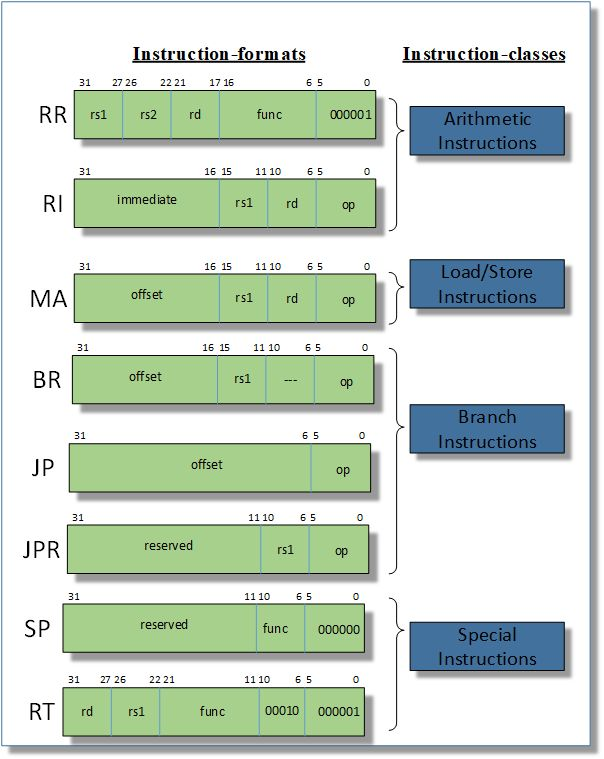
\includegraphics[width=0.9\textwidth]{src/images/3-3.png}
	\caption{Instruction Formats and Classes of the BROWSTD32 Architecture}
	\label{fig:fig33}
\end{figure}
\item
  \textbf{Special Registers:} Some registers in the general-purpose
  register file usually handle some special cases. However, contrary to
  the hard-wired zero-register \emph{r0}, any register, as long it is
  done consistent in the assembly file, can handle these other special
  cases. These special cases are the stack pointer (GPR\emph{1}), the
  frame pointer (GPR4) and the link register (\emph{GPR3}), which is
  then used as return address. For more details, please look into the
  Page-9 of Brownie Reference Manual \cite{RM}.
\item
  \textbf{Instructions:} for more details of the instruction and their
  syntax refer to Page-44 \cite{RM}
\end{itemize}
\begin{table}[!htb]
	\centering
	\begin{tabular}{|l|p{5cm}|l|p{5cm}|}
		\hline
		\multicolumn{1}{|c|}{\textbf{Instruction}} & \textbf{Description} & {\textbf{Instruction}} & \textbf{Description}                                                                       \\ \hline
		\emph{ADD, ADDI} & Add; Syntax: \emph{add rd rs0 rs1;} \emph{rs1} can
		alternatively be the immediate & \emph{SUB, SUBI} &
		Subtract\\\hline
		\emph{MUL} & Multiply & \emph{DIV, DIVU} & Divide\\\hline
		\emph{MOD, MODU} & Modulo & \emph{AND, ANDI} & And\\\hline
		\emph{OR, ORI} & Or & \emph{XOR, XORI} & Xor\\\hline
		\emph{LLS, LLSI} & Shift left logical & \emph{LRS, LRSI} & Shift right
		logical\\\hline
		\emph{ARS, ARSI} & Shift right arithmetic & \emph{ELT, ELTU} & Set
		``less than''; Syntax: \emph{slt rd rs0 rs1;} Compare \emph{rs0} and
		\emph{rs1} and set \emph{rd} to 1 if and only if rs0 is ``less than''
		rs1\\\hline
		\emph{LSOI} & Left shift \& OR immediate value & \emph{NAND,NOR} & Nand
		, NOR operation\\\hline
		\emph{ENEQ} & Set ``not equal'' & \emph{EEQ} & Set
		``equal''\\\hline
		\emph{LB} & Load Byte & \emph{LH} & Load High\\\hline
		\emph{LW} & Load Word; Syntax: \emph{load rd, imm(rs);} the effective
		address is computed by adding the immediate to \emph{rs} & \emph{SB} &
		Store Byte; Syntax: \emph{store imm(rd), rs;} the effective address is
		computed by adding the immediate to \emph{rd}\\\hline
		\emph{SH} & Store High & \emph{SW} & Store Word\\\hline
		\emph{BRZ} & Branch if ``equal zero'' Syntax: branch rs, imm; the branch target is a PC-relative address, given by the immediate
		& \emph{BRNZ} & Branch if ``not equal zero''\\\hline
		\emph{JP (JPR)} & Jump (Register); Syntax\emph{: j imm (jr rs);} The
		jump target is a PC-relative (absolute) address, given by the immediate
		(register) & \emph{JPL (JPLR)} & Jump and link (Register); Similar to
		\emph{j/jr}, but also writes the address from the following command to
		the link register; used for subroutine calls\\\hline
		\emph{NOP} & & \emph{RETI} & Return Interrupt\\\hline
		\emph{EXBW} & 8-bit to 32-bit sign extension & \emph{EXHW} & 16-bit to
		32-bit sign extension\\\hline
	\end{tabular}
	\caption{Summary of All Assembly Instructions in the \emph{browstd32} Processor}
	\label{fig:fig34}
\end{table}
\hypertarget{extending-dlxsim}{%
\section{Extending dlxsim}\label{extending-dlxsim}}
\hypertarget{startup-parameters-for-dlxsim}{%
\subsection{Startup Parameters for
dlxsim}\label{startup-parameters-for-dlxsim}}
Some parameters can be adapted when starting dlxsim. All mentioned
parameters in Figure 3‑5: do not allow blanks between a parameter, e.g.
``\emph{-pf0}'' instead of ``\emph{-pf~0}''.
\begin{table}[!htb]
	\centering
	\begin{tabular}{|p{3cm}|p{13cm}|}
		\hline
		\multicolumn{1}{|c|}{\textbf{Option}} & \textbf{Description}                                                               \\ \hline
		-f\emph{filename} & This parameter will load an assembly file after
		initialization. This parameter is equivalent to the instruction
		``\emph{load \{filename\}}'' in Figure 3‑7:.\\\hline
		-sf\emph{filename} & This parameter loads a script file that can contain
		any command that you can type within dlxsim. These commands are then
		executed one after the other. For simulation automation, you can forward
		the output of dlxsim to a file (\emph{make dlxsim {[}\ldots{]}
			\textgreater{} foo.txt}) and then extract the needed information out of
		this file (\emph{grep ``Total cycles'' foo.txt}).\\\hline
		-dbb\# (Debug Base Blocks)
		& This option only has an effect, if the later mentioned option
		``\emph{Debug Assembly}'' is enabled too. If both options are activated,
		then a register snapshot will automatically be printed at every base
		block start. This snapshot only includes registers, for which the value
		has changed since the last snapshot. By default, this option is turned
		off to avoid the enormous amount of output. To turn it on you have to
		enter \emph{``-dbb1}''.\\\hline
		-da\# (Debug Assembly) & 
		This option helps you debugging the simulated assembly code. A debugging
		output is printed for all load/store and jump/branch instructions,
		including in which cycle the message was printed and from which address
		it was triggered. By default, this option is turned on. To turn it off
		you have to enter \emph{``-da0}''.\\\hline
		-cdd\# (Check Data Dependency & 
		With this option, you enable a warning message that appears when an
		unresolved data dependency is found in the executed assembly code. This
		means you will get a warning if for example, \emph{r5} is read in cycle
		10, but an earlier command has made a write access to \emph{r5}, that
		cannot be read back before cycle 12. Therefore, you would read the `old'
		value. By default, this option is turned on. To turn it off you have to
		enter ``\emph{-cdd0}''.\\\hline
		-wsdo\# (Warn Specific Dependency Once) & 
		This option belongs to the before mentioned option Check Data
		Dependency. If there is an unresolved data dependency in a loop, then
		the warning message would usually be printed for every time the loop is
		executed. With this option defined, the warning will only be printed the
		first time the unresolved data dependency is noticed. By default, this
		option is turned on. To turn it off you have to enter
		\emph{``-wsdo0}''.\\\hline
		-pf\# (Pipeline Forwarding) & 
		With this option, you can configure, whether you have a ``Full
		Forwarding'' (1) or not (0). In case of forwarding, your operands are
		forwarded to next stages and no branch delay slot is required. But, even
		in case of forwarding, you still require a delay slot (nop) for
		loar/store.\\\hline
		-ms\# (Memory Size) & 
		The size of the memory that is available within dlxsim. It is the common
		memory for instructions and data.\\\hline
		-lf\emph{filename} & With this parameter, all print instructions for the
		LCD (as shown in Chapter~8.3.1) are written to a file instead of the
		screen.\\\hline
		-uf\emph{filename} & With this parameter, all print instructions for the
		UART (as shown in Chapter~8.3.2) are written to a file instead of the
		screen.\\\hline
		-af\emph{filename} & With this parameter, all outputs to the AudioOut
		IP-Core (as shown in Chapter~8.3.2) are written to a file instead of the
		screen.\\\hline
	\end{tabular}
	\caption{Summary of Helpful dlxsim Starting Parameters}
	\label{fig:fig35}
\end{table}
Legend: \emph{cursive}: replace with appropriate option, \#: replace
with a number

\hypertarget{how-to-add-a-new-instruction}{%
\subsection{How to Add a New
Instruction}\label{how-to-add-a-new-instruction}}
The following list shows you the needed steps to add a new instruction
for a given instruction-format. The given line numbers are rounded and
might change during time, as the source code is partially under
development. Every needed part of the source code is marked with a
comment that includes the string ``\emph{ASIP NEW\_INSTRUCTIONS}''.
\begin{enumerate}
\item
  \emph{dlx.h}:222 Add a new define for \textbf{OP\_\{CommandName\}}
  with a unique number.
\item
  \emph{sim.c}:227 Add the \textbf{name} for your assembly-command into
  the \textbf{operationNames}-array. The position of the name in this
  array has to correspond with the defined number in \emph{dlx.h} from
  the preceding step.
\item
  \emph{asm.c}:338 Add a new entry with your instruction name,
  instruction format and opcode into the \emph{\textbf{opcodes}}-table
  ``OpcodeInfo opcodes{[}{]}''. The \textbf{instruction name} has to be
  the same like in the previous step and completely written in
  lower-case! The already available \textbf{instruction formats} are
  shown in Figure 3‑6:. There are two different possibilities for the
  \textbf{opcode}. Either you use the only ``opcode'' or you use
  ``opcode'' and ``func'' field collectively. The unused bits always
  stay 0 in the opcode field. These two possibilities differ in how
  dlxsim is internally handling the instruction. This will become
  clearer in the following step. Have a look at the following step to
  find free opcodes. The following values in the opcode table are
  usually not that important and might be filled out by copy-and-paste
  from a similar instruction. Only the flags are important if you use
  instructions with immediate values as parameter. The flags are
  explained in \emph{asm.c}.
\item
  \emph{sim.c}:362 This step depends on your choice of the preceding
  step. You have used either the ``opcode'' or the ``opcode'' plus
  ``func'' field. If you have only ``opcode'' field, then you have to
  modify the \emph{\textbf{opTable}} in \emph{sim.c} otherwise in case
  of ``opcode and func'' field, then you have to modify the
  \emph{\textbf{specialTable}}. In both cases you replace the table
  entry at the position that corresponds to the chosen 6-bit opcode with
  your own \emph{\textbf{OP\_\{CommandName\}}}. So if you have chosen
  the opcode value 5, then you replace the 5\textsuperscript{th} entry
  (start counting with 0) in the array with your own command.
\item
  \emph{sim.c}:2197 Implement a new \textbf{case} for the big
  ``\emph{\textbf{switch (wordPtropcode)}}''-statement for your command.
  A good start is a copy-and-paste from a similar instruction. There are
  2 different variables for the parameters. For example, there is a
  ``\emph{\textbf{wordPtrrs1}}'' and a ``\emph{\textbf{rs1}}''. In
  ``\emph{\textbf{wordPtrrs1}}'' the number of the first source register
  is stored, while in ``\emph{\textbf{rs1}}'' the value of this source
  register is stored. At the beginning of an implementation of one
  specific ``\emph{\textbf{case}}'' some macros like
  ``\emph{\textbf{LoadRegisterS1}}'' are called. These macros take care,
  that ``\emph{\textbf{rs1}}'' is initialized with the current value of
  the register with the number ``\emph{\textbf{wordPtrrs1}}''.
\item
  Compiling: To test your modified version of dlxsim you have to
  re-compile it. Simply type ``make'' in the dlxsim directory.
\end{enumerate}
When the error ``\emph{Unknown Opcode}'' occurs while loading the
assembly file, then the corresponding instructions was not accepted. If
you are sure, that it is not a typing error in the assembly file
(register names, immediate values, \ldots) then have a look into points
1 -- 4.
\hypertarget{how-to-add-a-new-instruction-format}{%
\subsection{How to Add a New
Instruction-Format}\label{how-to-add-a-new-instruction-format}}
Adding a new instruction format is much more difficult than adding a new
instruction for a given format. To add a new format you have to take
care about how the parameters for your new format are to be stored in a
32-bit instruction word and how they are extracted out of it. Every
needed part of the source code is marked with a comment that includes
the string ``ASIP NEW\_FORMAT''.
\begin{enumerate}
\item
  \emph{asm.c:}140 Define a unique number for your instruction-format
\item
  \emph{asm.c:}150 Add the \emph{min} and \emph{max} numbers of
  arguments, that your instruction format accepts in the arrays
  ``\textbf{minArgs}'' and ``\textbf{maxArgs}''. Use the position in the
  array, that corresponds to the defined number in the previous step.
\item
  \emph{asm.c:}765 Implement how the parameters will be stored in the
  32-bit instruction word within the ``\textbf{switch
  (insPtr-\textgreater class)}''-statement.
\item
  \emph{asm.c}:1080 Implement what will be written if the instruction is
  disassembled in the ``\textbf{switch
  (opPtr-\textgreater class)}''-statement.
\item
  \emph{sim.c:}2215 In the method ``\textbf{compile}'' you have to
  implement how the 32-bit instruction word will be expanded.
\item
  Compiling To test your modified version of dlxsim you have to
  re-compile it. Simply type ``make'' in the dlxsim directory.
\end{enumerate}
\begin{table}[!htb]
	\centering
	\begin{tabular}{|l|p{13cm}|}
		\hline
		\multicolumn{1}{|c|}{\textbf{Instruction Format}} & \textbf{Parameters}                                                               \\ \hline
		NO\_ARGS & no operands\\\hline
		LOAD & (register, address)\\\hline
		STORE & (address, register)\\\hline
		LUI & (dest, 16-bit expression)\\\hline
		ARITH\_2PARAM & (dest, src) OR (dest, 16-bit immediate) OR "dest"
		replaced by "dest/src1"\\\hline
		ARITH\_3PARAM & (dest, src1, sr2c) OR (dest/src1, src2) OR (dest, src1,
		16-bit immediate) OR (dest/src1, 16-bit immediate)\\\hline
		ARITH\_4PARAM & (rd, rs1, rs2, rs3) OR (rd, rs1, rs2, 5-bit
		immediate)\\\hline
		BRANCH\_0\_OP & (label) the source register is implied\\\hline
		BRANCH\_1\_OP & (src1, label)\\\hline
		BRANCH\_2\_OP & (src1, src2, label)\\\hline
		JUMP & (label) OR (src1)\\\hline
		SRC1 & (src1)\\\hline
		LABEL & (label)\\\hline
		MOVE & (dest,src1)\\\hline
	\end{tabular}
	\caption{Summary of Available dlxsim Instruction Formats}
	\label{fig:fig36}
\end{table}
\hypertarget{using-dlxsim}{%
\section{Using dlxsim}\label{using-dlxsim}}

Dlxsim is distributed as source code, so before using it you have to
compile it. Usually this is done, by just typing ``\emph{make''} in the
``\emph{tcl''} subdirectory and afterwards in the ``\emph{dlxsim''}
directory. Then you can start the program by typing ``dlxsim''. If you
want to use dlxsim for an ASIP Meister Project, then you have to set
``\emph{DLXSIM\_DIR}'' (see Table \ref{fig:fig25}) to
the path where dlxsim is located e.g.
"\emph{/home/ces-asip00/epp/dlxsim\_Laboratory}'', and then typing
``\emph{make dlxsim}'' in an application's subdirectory.

Figure 3‑7: shows some typical dlxsim commands. The list is not
exhaustive, but it covers all the usual suspects.
\begin{table}[!htb]
	\centering
	\begin{tabular}{|p{3cm}|p{13cm}|}
		\hline
		\multicolumn{1}{|c|}{\textbf{Command}} & \textbf{Description}                                                               \\ \hline
		load \emph{filename\textsuperscript{+}} & Load a file, parse its
		content, and place the translated content to the simulated memory. Every
		address that is not mentioned in the file remains it old
		value.
		\\ \hline
		get \emph{address} \{\emph{options}\} & 
		Examples for ``\emph{address}'' are \emph{r0}\ldots{} \emph{r31},
		\emph{pc}, \emph{npc} (next pc), 10 (memory address 10), 0x10 (memory
		address 16), \_main (if \_main is a label).
		Examples for ``\emph{options}'' are: u (unsigned), d (decimal), x
		(hexadecimal, default), B (binary), i (instruction), v (do not read a
		value, but print the address itself; as example this can be used to
		translate from decimal to binary), s (interpret the upcoming sequence as
		0-terminated string). In the options, you can also request to get the
		succeeding addresses from the determined base address. As an example,
		``\emph{get \_loop 10i}'' would deliver the 10 first commands from the
		label \emph{\_loop} interpreted as instruction memory. This also works,
		if the address is a register, e.g. ``\emph{get r1 5u}''.\\\hline
		put \emph{address data} & Place some data at the given address. The
		address might be a register too, like in the ``\emph{get''}
		command.\\\hline
		step \{\emph{number}\} & Execute the next number of instructions given
		by ``\emph{number}'', the default value is 1. The printed assembly
		command at the end of ``\emph{step}'' is the next assembly command that
		is to be executed.\\\hline
		go \{\emph{address}\} & Execute the assembly program, until an error
		occurs or a trap instruction is executed. It starts executing at
		``\emph{address}''. If no ``\emph{address}'' is given, then it continues
		executing where it is stopped (e.g. after some single steps). The
		default address is 0.\\\hline
		stats \{\emph{options}\} & Print some statistics about the simulated
		assembly program. The \emph{options} are explained in more detail in
		Chapter~3.3.1.\\\hline
		quit,exit & Terminates the program\\\hline
		stop \{\emph{options}\} & Manages break points:
		``\emph{stop at address \{command\}}'': Executes ``\emph{command}''
		whenever the given ``\emph{address}'' is touched in any way. The default
		``\emph{command}'' is to abort the execution.
		``\emph{stop info}'': prints the list of break points.
		``\emph{stop delete number\textsuperscript{+}}'': deletes some specific
		break points. The numbers are according to the ``\emph{stop info}''
		list.\\\hline
		asm ``\emph{command}'' \{\emph{pc}\} & Return the opcode for
		``\emph{command}''. If the command needs to know the address where it is
		to be stored (e.g. pc-relative jumps), then the current pc can be given.
		Default pc is 0.\\\hline
	\end{tabular}
	\caption{Summary of Typical dlxsim Commands}
	\label{fig:fig37}
\end{table}
\textbf{Legend}: \emph{cursive}: replace with appropriate option,
\{braces\}: optional, \textsuperscript{+}: one or multiple times

Some more points that have to be mentioned about dlxsim are:

\begin{itemize}
\item
  You can use the cursor buttons to navigate in your command history,
  i.e. in the previously entered commands. The up- and down-arrow-keys
  let you navigate inside the selected command, e.g. to correct typing
  errors.
\item
  When you just enter an empty command in dlxsim (i.e. just press enter
  without having entered a command), then the last executed command will
  be repeated. This is for example useful, when you want to step through
  your code. You just have to execute the step instruction one time
  manually by typing ``\emph{step}'' in the shell and afterwards you can
  repeatedly press enter to execute the next step instructions.
\item
  When you press the Tab key, you will get an auto completion for
  filenames. The offered files are the files in the directory from where
  you started dlxsim. Although this auto completion will support the
  abbreviation ``\emph{\textasciitilde{}}'' for your home directory, a
  load instruction with this abbreviation will fail. The same holds for
  loading files with the ``\emph{-f}'' starting parameter, as shown in
  Figure 3‑7:.
\item
  After you have simulated an assembly code, you have to restart dlxsim
  to simulate another assembly code. The ``\emph{load}'' instruction
  will not reset everything to its default value.
\item
  Every assembly command that accepts an immediate value as parameter
  can also handle a label as immediate value. This is especially useful
  for the load/store, branch/jump and lhi commands.
\item
  The ASIP Meister unit for data memory access does not accept an
  immediate change from a load command to a store command or vice versa.
  Dlxsim can handle this situation, but will print a warning to
  indicate, that this assembly code might produce a different result if
  it is simulated with the VHDL-code from an ASIP Meister CPU.
\end{itemize}

\hypertarget{statistics}{%
\subsection{Statistics}\label{statistics}}

There are many statistics available for the executed assembly code. You
can get the statistics by typing ``stats \{\emph{options}\}'', as shown
in Figure 3‑7:. The different available options are shown in Figure
3‑8:. The different options may be combined; the default option is
``\emph{all}''.

\hypertarget{debugging-with-dlxsim}{%
\subsection{Debugging with dlxsim}\label{debugging-with-dlxsim}}

This chapter assumes, that you are not only used to the assembler code
and dlxsim, but that you are also used to the compiler and inline
assembly (see Chapter~8).

\textbf{General Points:}

\begin{itemize}
\item
  \begin{quote}
  \textbf{Compare the results} from the GCC compiled version and the
  gcc-compiled version. For the gcc compiled version you have to add
  printf statements for all essential variables, like:
  \end{quote}
\end{itemize}

\#ifndef GCC

printf(``temp1: \%i\textbackslash n'', temp1);

\#endif

\begin{quote}
For the GCC-compiled version, you have to make the important variables
global, for example moving the variable ``\emph{temp1}'' from inside the
main method to a global part outside the main method. All global
variables will get an own label in the assembly code with an underscore
before the name, e.g. the variable ``\emph{temp1}'' will get the label
``\emph{\_temp1}''. In dlxsim you can see the value of global variables
with the ``\emph{get}'' instruction, e.g. ``\emph{get \_temp1 i}''.
\end{quote}
\begin{table}[!htb]
	\centering
	\begin{tabular}{|p{2cm}|p{14cm}|}
		\hline
		\multicolumn{1}{|c|}{\textbf{Option}} & \textbf{Description}                                                               \\ \hline
		hw & Shows the memory size.\\\hline
		stalls & Shows the pipeline stalls (i.e. number of elapsed cycles, where
		the pipeline did not proceed) for the different
		categories.\\\hline
		all & Shows all statistics in the same order as they appear in this
		table.\\\hline
		reset & Resets all statistics to their initial values. This is useful if
		you want to see statistics for a specific part of the program and you
		want to mask the statistic results that are computed before you reach
		specific program part.\\\hline
		imcount, imcount2, imcount3 & 
		Shows the number of executions for memory addresses. The output is
		organized into three columns. The first column shows how often a
		specific part of the instruction memory was executed. The second column
		shows the starting address of the specific memory part and the third
		column shows the size of the memory part. The different spellings of
		imcount (e.g. imcount2) refer to different sorting for the columns. This
		statistic merges neighbored memory addresses that are executed for
		nearly the same number into a single memory portion for which one output
		line is printed. The deviation to the average value is printed in the
		first column (e.g. ``\# of executions: 2 ± 1'').\\\hline
		baseblocks & Shows the separation from the program into base blocks.
		This statistic is separated into 4 columns. The first one shows the
		start address and the reason why a base block starts there (e.g. a
		label, the command after a branch command, \ldots). The second row shows
		the end address together with the reason why the base block ends there.
		The third row shows the size of the base block and the last row shows
		how often it was executed.\\\hline
	\end{tabular}
	\caption{Summary of Available dlxsim Statistics}
	\label{fig:fig38}
\end{table}
\begin{itemize}
\item
  \begin{quote}
  Sometimes the \textbf{dlxsim simulation aborts} with an error message,
  e.g. when a load instruction is trying to access an address that is
  outside the simulated memory range. In such cases, you first have to
  find out, which instruction is causing this crash. With the
  instruction ``\emph{get pc}'' you can see the address which is
  currently executed. With the instruction ``\emph{get \{address\} i}''
  you can see which instruction is placed at this address and at which
  label this instruction can be found. With the instruction ``\emph{get
  \{Address\}-0x10 20i}'' you can see the context of this instruction.
  \end{quote}
\item
  \begin{quote}
  Getting more debugging information from dlxsim is very helpful to
  understand, what the assembly code is doing. Therefore, the dlxsim
  starting parameters \emph{``‑da\#''} and \emph{``‑dbb\#}'' are useful.
  You have to replace the ``\#'' with either a ``1'' to turn the option
  on or with a ``0'' to turn it off.
  \end{quote}
\item
  da\#: Debug Assembly. This option is turned \emph{on} by default and
  it will print status information on the screen for every
  jump/branch/load/store-instruction. You can print additional status
  information by adding your needed information into the
  ``\emph{sim.c}'' of dlxsim.
\item
  dbb\#: Debug Base Blocks. When you turn \emph{on} this option then at
  every start of a base-block all changed register values will be
  printed. A base block is an elementary block of assembly code that is
  only executed sequentially. This means, that either all instructions
  of a base block are executed (one after the other) or none of them is
  executed at all. The borders of a base block (beginning/end) are jumps
  and labels. The simulation will create a huge amount of output on the
  screen if you turn this option on. Therefore it is recommended, that
  you copy the output to a text file for easier reading. You can
  automatically print everything into a text file if you start dlxsim
  like:\\
  \emph{``make dlxsim DLXSIM\_PARAM=''‑fassembly.dlxsim ‑dbb1''
  \textbar{} tee output.txt''}\\
  The ``\emph{tee}'' program will copy all output to the screen and to
  the file.
\item
  \begin{quote}
  Always have a look at the printed warnings when dlxsim runs the
  simulation. At the end of every simulation the warnings are
  summarized, i.e. the number of the printed warnings is shown. If the
  simulations aborts before its usual end this summary is not printed.
  To see the summary you can see them in the statistics with
  \emph{``stats warnings''}.
  \end{quote}
\end{itemize}
 
\hypertarget{asip-meister}{%
\chapter{ASIP Meister}\label{asip-meister}}
ASIP Meister \cite{ASIPMeister} is a development environment for creating
application specific instruction set processors (ASIPs). It is not the
purpose of this chapter to explain the benefits or the usage of ASIP
Meister. To learn the usage of ASIP Meister you have to work through the
user manual and the tutorial, which are available in the ``share''
subdirectory of ASIP Meister. ASIP Meister itself is located in the
directory /AM/ASIPmeister/ in our laboratory environment. The purpose of
this chapter is to summarize some typical challenges with ASIP Meister
and some typical but hard to understand error messages, that might
appear while using the software. Chapter 4.4 will afterwards give a
tutorial about the so-called `Flexible Hardware Model' (FHM) of ASIP
Meister, as this part is missing in the official tutorial.
\hypertarget{what-is-asip-meister}{%
\section{What is ASIP Meister?}\label{what-is-asip-meister}}
ASIP Meister is a tool for developing Application Specific Instruction
Set Processors (ASIPs) from high level specification description. The
functionality of the tool is listed below:
\begin{itemize}
\item
  Automatic generation of the processor HDL description from Micro Op.
  description.
\item
  Fast Estimation of processor design quality at an early stage of
  design process.
\end{itemize}
\begin{figure}[!htb]
	\centering
	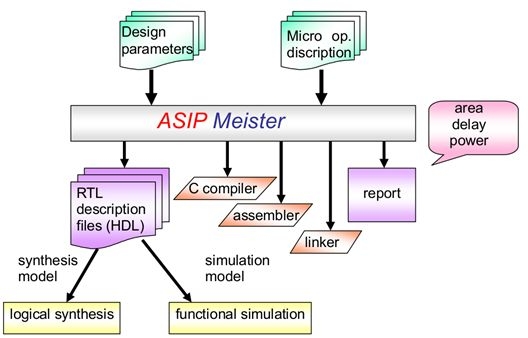
\includegraphics[width=0.9\textwidth]{src/images/4-1.png}
	\caption{ASIP Meister Input and Output}
	\label{fig:fig41}
\end{figure}
For the above functionality, it is possible to examine and compare
different architecture implementations using ASIP Meister. The
input/output of ASIP Meister is roughly shown in the figure below. Using
the GUI of ASIP Meister, the user inputs the design parameters and Micro
Op. description. ASIP Meister generates an estimation report of the
processor design quality and its RTL description files. Furthermore,
ASIP Meister also generates a development environment composed of a C
compiler, assembler and linker. The synthesis model and the simulation
model are automatically generated in HDL. These models then become the
input to logical synthesis tools and functional simulation tools.
\hypertarget{processor-design-flow-using-asip-meister}{%
\section{Processor Design Flow Using ASIP
Meister}\label{processor-design-flow-using-asip-meister}}
Open each sub-window in ASIP Meister, in the order specified in Figure
4-2. This would be typically the order of operation that should be
performed to design and generate a processor core using ASIP Meister.
\begin{figure}[!htb]
	\centering
	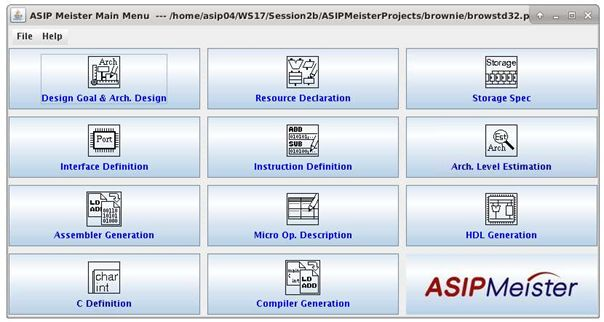
\includegraphics[width=0.9\textwidth]{src/images/4-2.png}
	\caption{ASIPmeister main window}
	\label{fig:fig42}
\end{figure}

1. \textbf{Design Goal \& Arch. Design}: Setting design goal values and
pipeline stages

2. \textbf{Resource Declaration}: Declaring resources

3. \textbf{Storage Specification}: Definition Specifying storages

4. \textbf{Interface Definition}: Defining I/O interfaces of the target
processor

5. \textbf{Instruction Definition}: Defining instruction types and
instruction set

6. \textbf{Arch. Level Estimation}: Estimating design quality of target
processor

7. \textbf{Assembler Generation}: Generating Assembler description files

8. \textbf{Micro Op. Description}: Describing micro-operations for each
instruction

9. \textbf{HDL Generation}: Generating HDL files of target processor

10. \textbf{C Definition}: Defining C code

11. \textbf{Compiler Generation}: Generating compiler and Binutils

For details of the individual sub-windows, see the corresponding
sections in {[}TUT{]} and {[}UM{]}.

\hypertarget{typical-challenges-while-working-with-asip-meister}{%
\section{Typical Challenges while Working with ASIP
Meister}\label{typical-challenges-while-working-with-asip-meister}}

\begin{itemize}
\item
  The \textbf{register r0} is hardwired to zero in our ASIP Meister CPU.
  Nevertheless, this is only a hint for the compiler. The compiler will
  never try to write a value different from zero to this register and
  the compiler will use this register when a zero value is needed.
  However, this register can be written with any value, like all the
  other registers. The reason for this behavior is that the register
  file is created by the FHM description (flexible hardware model) in
  the ``\emph{Resource Declaration}'', and the configurations in the
  ``\emph{Storage Specifications}'' are only used for the compiler and
  assembler, but are not used for creating the hardware.
\item
  Do not use the ``\emph{meister/xxx.sim}'' directory like
  ``\emph{browstd32.sim}'', when simulating or synthesizing the VHDL
  code. There is a problem with the register file. Instead, use the
  ``\emph{meister/xxx.syn}'' directory like ``\emph{browstd32.syn}''.
  The same VHDL-code will be used for synthesis as explained in
  Chapter~6.
\item
  ASIP Meister can only be used once on each computer. Therefore, if two
  different groups want to work with ASIP Meister, they have to use
  different computers. To make sure, that ASIP Meister is at most
  started once on each PC, the starting script tests, whether the file
  ``\textbf{/tmp/fhm\_server.log}'' exists in the temporary directory.
  ASIP Meister creates this file while starting and it is removed after
  ASIP Meister terminates. If this file exists, then someone else might
  already use ASIP Meister on that PC. However, it can also happen, that
  this file is not automatically deleted, after ASIP Meister terminates.
  If you think, that no one else is using ASIP Meister on this PC, then
  remove this file.
\item
  When writing \textbf{MicroOp} code, be careful with macros. A macro
  that is defined as three stage long and started in the ID phase will
  execute in the ID, the EX and the MEM phases, not just in the ID
  phase. If you want to view an instruction's \emph{MicroOp} code
  without macros, select this instruction and hit the ``\emph{Macro
  Expansion}'' button in the upper right corner.
\end{itemize}

\hypertarget{tutorial-for-the-flexible-hardware-model-fhm}{%
\section{Tutorial for the ``Flexible Hardware Model''
(FHM)}\label{tutorial-for-the-flexible-hardware-model-fhm}}

To add a new instruction to an ASIP Meister CPU one would usually write
a \emph{MicroOp} description for the instruction, using the facilities
of an existing hardware module (ALU, shifter, adder, etc.) The ability
to use multiple hardware modules during one stage and to create more
than one instance of a specific module combined with the operators
provided by the \emph{MicroOp} description language is sufficient for
most basic instructions. However, this method has several shortcomings
that make it impossible to do the following (among others):

\begin{itemize}
\item
  Working with not program-defined wire ranges which depend on register
  contents or immediate values
\item
  Implementing multi-cycle instructions
\end{itemize}

This tutorial will show how to write a new hardware module to provide a
"\emph{rotate left}" instruction.

\hypertarget{setting-up-asip-meister-to-add-new-fhm}{%
\subsection{Setting up ASIP Meister to add new
FHM}\label{setting-up-asip-meister-to-add-new-fhm}}

In our current setup, ASIP Meister is installed globally. To modify FHMs
you will need to set it up locally:

\begin{enumerate}
\def\labelenumi{\arabic{enumi}.}
\item
  Copy the ASIP Meister directory tree to your home directory:
\end{enumerate}

\begin{lstlisting}
cp -r /AM/ASIPmeister/~
\end{lstlisting}

\begin{enumerate}
\def\labelenumi{\arabic{enumi}.}
\setcounter{enumi}{1}
\item
  Update the PATH environment variable to use the local ASIP Meister
  directory by editing the file \emph{\textasciitilde/.bashrc.user} and
  adding the following line at the end of the file:
\end{enumerate}

\begin{lstlisting}
PATH=\$HOME/ASIPmeister/bin/:\$PATH
\end{lstlisting}

\begin{enumerate}
\def\labelenumi{\arabic{enumi}.}
\setcounter{enumi}{2}
\item
  Force the shell to re-read the \emph{bashrc} file to use the updated
  PATH variable:
\end{enumerate}

\begin{lstlisting}
source ~/.bashrc or logout and login again
\end{lstlisting}

\begin{enumerate}
\def\labelenumi{\arabic{enumi}.}
\setcounter{enumi}{3}
\item
  Verify that you are using the correct ASIP Meister copy: \emph{``which
  ASIPmeister''} should print the path to the local copy
\item
  Edit \emph{\textasciitilde/ASIPmeister/bin/ASIPmeister} (line 25) and
  make sure your local ASIP Meister path (\emph{\$HOME/ASIPmeister}) is
  assigned to the variable \emph{ASIP\_MEISTER\_HOME}.
\end{enumerate}

From now on whenever relative paths (not starting with a /) are
mentioned, \emph{\$HOME/ASIPmeister} should be the base directory, i.e.:
\emph{share/­fhmdb/­workdb/­peas/­rotator.fhm} should be
/\emph{home/­asipXX/­ASIPmeister/­share/­fhmdb/­workdb/­peas/­rotator.fhm}

\hypertarget{fhm-structure}{%
\subsection{FHM structure}\label{fhm-structure}}

The directory \emph{share/fhmdb} has two subdirectories and the file
\emph{fhmdbstruct}. ASIP Meister reads this file to determine which FHM
files to use. Most of the modules necessary for the basic functions of
the CPU are in the directory \emph{basicfhmdb}; they are further divided
into the categories \emph{computational} and \emph{storage}. New FHMs
should be added to the \emph{share/­fhmdb/­workdb/­peas} directory.

FHMs are written in XML (eXtensible Markup Language). ASIP Meister
processes their data in several stages, most importantly ``\emph{HDL
Generation''} which creates the CPU VHDL files. Usually some embedded
Perl is used in the FHMs to customize VHDL code. An FHM can be divided
roughly into two parts: \emph{behavior} and \emph{synthesis}. We are not
going to differ between them, though.

\textbf{Header and Function description}

First, we need to make ASIP Meister aware of our new FHM. Edit
\emph{share/­fhmdb/­fhmdbstruct}. Go to the tag \emph{\textless library
name="workdb"\textgreater{}} and add another model to the peas class by
adding the line
\emph{\textless model\textgreater rotator\textless/model\textgreater{}}.
Save and close the file, as this is the only change needed for this
file.

To make your task a bit easier, we have prepared a template file with
many mandatory sections already done. Copy the file
\emph{home/ces-asip00/epp/workdb/peas/skeleton-1p.fhm} to
\emph{share/fhmdb/workdb/peas/rotator.fhm} and edit this file. TAKE
CARE: Small errors in this file will lead to very general error messages
that are hard to find. Consider the general hint in Chapter~4.6 and
double-check your changes for typing errors and missing spaces.

Name your FHM ``\emph{rotator}'' by editing the name in the
\emph{\textless model\_name\textgreater{}} tag. Rename the author in the
\emph{\textless author\textgreater{}} tag. The
\textless parameter\textgreater{} section is used to allow FHM
customization from the \emph{Resource declaration} section in ASIP
Meister. The parameter \emph{bit\_width} for the input and output vector
is already defined. Leave it as it is.

Next, we have the \emph{function description}, which is generated with
an embedded Perl script. Functions are used by ASIP Meister to interface
the MicroOp description and the actual VHDL code. The program generates
the necessary registers/multiplexers and control signals to address the
corresponding hardware module. The Perl script uses the Perl
\emph{print} function to output the \emph{function description}. The 
\emph{\textless\textless{}} and the following string start a so called
``\emph{here document''}, which instructs the Perl interpreter to treat
all the following lines as single character string (performing variable
substitution) until it finds the string after the
\emph{\textless\textless{}} on a single line.

Rename the name of the \emph{function} from "\emph{foo}" to
"\emph{rotl}" and change the comment in the line above to something
sensible (e.g. "\emph{rotate left}").

Functions are divided into 4 blocks:

\textbf{input:} declaration of \emph{function parameters}. We need the
actual data and the amount by which to rotate, so write the following
two lines between the curly braces of \emph{input}:
\begin{lstlisting}
bit [$msb:0] data_in;
bit [7:0] amount;
\end{lstlisting}
\begin{quote}
Note that \emph{\$msb} is a Perl variable that will be substituted by
the actual value (assigned above, \emph{\$bit\_width - 1})
\end{quote}

\textbf{output:} declaration of the \emph{function output}. The rotated
value is of the same type as the input value, so add the following
between the braces of the \emph{output} block:
\begin{lstlisting}
bit [$msb:0] data_out;
\end{lstlisting}
\textbf{control:} \emph{control variables} used by the RTG controller of
the CPU. These signals are not accessible from the MicroOp description,
but can be used in the VHDL code in the FHM. For our hardware to know
which direction (left or right) to shift, we will use a 1 bit signal
('0' for left, '1' for right). Add the following for the \emph{control}
section:
\begin{lstlisting}
in direction;
\end{lstlisting}
\begin{quote}
The \emph{in} keyword means that the module will be able to access the
signal read-only. \emph{out} and \emph{inout} are the other two
possibilities.
\end{quote}

\textbf{protocol:} Describes what the \emph{function} should do once a
condition is met. In this case, we will use the following simple
protocol:
\begin{lstlisting}
[direction == '0'] {
	valid data_out;
}
\end{lstlisting}
That is, it is for the \emph{function description}. The \emph{function
convention} is next. The content is identical to the \emph{function
description} except for the following two changes:

\emph{Write the following into the protocol} block:
\begin{lstlisting}
single_cycle_protocol {
	direction = '0';
}
\end{lstlisting}
Write the following into the \emph{control} block:
\begin{lstlisting}
in bit direction;
\end{lstlisting}
To declare additional \emph{functions}, simply add their descriptions to
the ``\emph{here document}'' (or use a new print statement), do not
start a new XML \emph{\textless function\_description\textgreater{}} or
\emph{\textless function\_conv\textgreater{}} block.

\textbf{Ports, Instance and Entity}

The \emph{\textless function\_port\textgreater{}} section declares the
signals that will be connected to our module. As with the \emph{function
convention} and \emph{function description} it is an embedded Perl
script, and as before the output is done with the ``\emph{here
document''}. We mentioned all the needed ports in the \emph{function
convention} and \emph{description} already: \emph{direction},
\emph{data\_in}, \emph{amount}, \emph{data\_out}. Use the following
lines for the declaration (make sure you write them between the
``\emph{print \textless\textless FHM\_DL\_PORTS;''} and the
``\emph{FHM\_DL\_PORTS lines}'' in the
\emph{\textless function\_port\textgreater{}} part):
\begin{lstlisting}
direction	in	bit	mode
data_in	in	bit_vector	$msb	0	data
amount	in	bit_vector	7	0	data
data_out	out	bit_vector	$msb	0	data
\end{lstlisting}
You will notice two things: First, there are two types of ports: mode
and data ports\footnote{There is another type: ctrl which is used for
  multi cycle instructions} - use \emph{data} for your input and output
signals and \emph{mode} for control signals. Second, one bit signals are
declared as bit and don't have a range specification, while signals
wider than one bit (vectors) are of type \emph{bit\_vector} and have a
range (width) - in this case from the most significant bit down to 0.

The \emph{\textless instance\textgreater{}} is the core of the module -
the actual architecture VHDL code. Embedded Perl is used here as well.
Go to the \emph{\$signals} variable. As you can see here, documents can
also be used to assign values to variables. No additional signals are
necessary for our rotator, so we will leave \emph{\$signals} as it is.

The next variable, \emph{\$vhdl} is more interesting: Our module should
be sensitive to changes of input data, shifting amount and shifting
direction (so it should re-compute the output data if one of these three
values changes), hence we define a process with these three values in
its sensitivity list. We also need one integer variable to hold the
value of the shifting amount (\emph{amount} is a signal, not a variable)
and one signal for the temporary value of the result. After the
\emph{begin} keyword we can write the process code. Remember that this
variable (as all the others) will later be used to create the actual
VHDL output (the variable is not placed at the correct position for the
VHDL output, but instead it is later used at the correct position). If
you are writing statements that span multiple lines you have to
encapsulate them with double quotes (``\,'') to assign them to the
variable.

First, we need to convert the signal \emph{amount} to integer and assign
it to \emph{a}. Next we check if \emph{a} is within range, if it is not,
we set the result to \emph{undefined}, otherwise we can rotate. A case
switch is used to decide into which direction to rotate. The
\emph{others} case is necessary, as the type \emph{std\_logic} has more
states than just '0' and '1', so don't delete it when you add the code
for "rotate right".

At the end of the process, we assign the value of the \emph{res} signal
to the \emph{data\_out} signal. See below listing for the architecture
VHDL:
\begin{lstlisting}
process (data_in, amount, direction)
variable a   : integer;
variable res : std_logic_vector($msb downto 0);
begin
a := TO_INTEGER(UNSIGNED(amount));
if (a > 0 and a < $bit_width) then
case direction is
when '0' => -- rotate left
res($msb downto a) :=
data_in($msb - a downto 0);
res(a - 1 downto 0) :=
data_in($msb downto $bit_width - a);
when others => -- not reached
res := (others => 'X');
end case;
else
res := (others => 'X');
end if;
data_out <= res;
end process;
\end{lstlisting}
Leave the comment section untouched and look closer at the
FHM\_DL\_TOP\_2 document. First, three libraries are included - these
are necessary for the std\_logic data types and several functions and
macros. Next, the entity is declared, which states all input and output
ports of our VHDL module. Although we already defined the ports of our
FHM, these were interpreted by ASIP Meister - the port declaration for
the entity, as well as the rest of the VHDL code will be used verbatim,
without any error checking by ASIP Meister (although we can still check
for errors in ModelSim). Use the code in the below listing (between the
``\emph{print \textless\textless FHM\_DL\_PORTS;''} and the
``\emph{FHM\_DL\_PORTS lines}'' in the
\emph{\textless instance\textgreater{}} part) for the entity ports:
\begin{lstlisting}
data_in   : in  std_logic_vector($msb downto 0);
direction : in  std_logic;
amount    : in  std_logic_vector(7 downto 0);
data_out  : out std_logic_vector($msb downto 0)
\end{lstlisting}
That is for the \emph{\textless instance\textgreater{}} block. Next, we
have an \emph{\textless entity\textgreater{}} section. It defines an
\emph{entity} in a different file, which is why a new block is needed,
but the ports are the same, so use the code from the above listing.

\hypertarget{estimation-and-the-synthesis-model}{%
\subsection{Estimation and the Synthesis
Model}\label{estimation-and-the-synthesis-model}}

The \emph{\textless testvector\textgreater{}} section may be left empty,
the \emph{\textless synthesis\textgreater{}} script contains
instructions to process the FHM file - we leave that untouched as well.

The \emph{\textless estimation\textgreater{}} block has data relevant
for area, power and delay estimations, but we use more accurate tools,
that consider the actual application execution, as shown in Chapter~6.5,
and Chapter~7.2. Leave the estimation data there though, as ASIP Meister
will complain without them. You should change FHM parameters however,
you will have to adjust the estimation section if you want to get rid of
the warnings.

That is it for the \emph{behavior} model. As mentioned in the beginning,
we won't differ between the \emph{behavior} and the \emph{synthesis}
model, so just copy-and-paste the complete
\emph{\textless model\textgreater{}} block and change the value of the
\emph{\textless design\_level\textgreater{}} tag from behavior to
synthesis.

Your FHM file should now have a structure similar to the following
listing:
\begin{lstlisting}
<?xml version="1.0" encoding="Shift_JIS" ?>
<FHM>
<model_name> rotator </model_name>

<model>
<design_level> behavior </design_level>
[...]
</model>

<model>
<design_level> synthesis </design_level>
[...]
</model>
</FHM>
\end{lstlisting}
You can now use the module in ASIP Meister. Instantiate the FHM resource
in the \emph{Resource Declaration} and write the new instruction
\emph{rotl}. Set the operands to the correct Addressing Mode, DataType,
etc in the \emph{Behavior Description} window, but leave the behavior
description itself out. Use the syntax
\begin{lstlisting}
result = ROT0.rotl(source0, am);
\end{lstlisting}
where \emph{result} and \emph{source0} are 32-bit wires and \emph{am} is
a 8-bit wire.

\hypertarget{testing-the-new-fhm}{%
\subsection{Testing the new FHM}\label{testing-the-new-fhm}}

When HDL and SWDev Generation run without errors (SWDev will probably
print some warnings about setting throughput to 1 - that is alright),
proceed testing your module/instruction. Write a small assembly code,
compile it (as shown in Table \ref{fig:fig22}), create a
new project in ModelSim, load your design and compile it. If there are
errors during compilation of the VHDL files (especially in
\emph{fhm\_rotator\_w32.vhd)}, then you have made a mistake in your VHDL
code. Now you could go back to the FHM and correct it there, but a
faster way is to edit the mentioned VHDL file in your
\emph{\textasciitilde/ASIPMeisterProjects/­browstd32\_YourCPU/­meister/­browstd32\_YourCPU.syn/}
directory and try to correct the code there. Once you get it running,
make the corrections in the FHM file as well (important: in the behavior
{and} synthesis sections), as ASIP Meister will overwrite the VHDL files
every time you recreate the CPU.

Once your CPU VHDL files are compiled, run your test program. Check the
results carefully! Experiment with large values as well (i.e. use
\emph{lhi \%r2, \$65535} to set the upper 16 bits to '1'). Once you
verified your design, backup your FHM (important!) and implement the
``\emph{rotr} `` - right rotation instruction by making the necessary
changes to your FHM.

\hypertarget{multi-cycle-fhms}{%
\section{Multi Cycle FHMs}\label{multi-cycle-fhms}}

As mentioned at the beginning of the tutorial, one of the reasons to
write custom FHMs is to implement multi-cycle (stalling) instructions.
Examples of stalling instructions are the multiplication and division
operations, which use dedicated multiplier and divider hardware blocks.
Stalling hardware is usually implemented with \emph{State Machines}.
This section will show you how to write a FHM for a multi-cycle
instruction. We will extend the rotator from the previous sections - the
multi-cycle version will rotate only one bit per cycle (obviously the
performance will be inferior to the single-cycle variant; it is just for
demonstration).

ASIP Meister provides three signals to control multi-cycle instructions:
\emph{start}, \emph{fin} and \emph{cancel}. The \emph{start} signal will
be set by the RTG controller once the instruction is started, and our
hardware will set the \emph{fin} signal once the operation is finished,
to signal the CPU that normal pipeline operation can be resumed. If a
\emph{cancel} signal arrives, the hardware should abort its operation.
We will disregard the cancel signal here, but reset our hardware on the
CPU \emph{reset} signal into its default state.

\textbf{\textless function\_description\textgreater{}}

We need to define the three control signals in the \emph{control} block
of our function. As the \emph{control} block of your function use
\begin{lstlisting}
in  start, cancel, direction;
out fin;	
\end{lstlisting}
We also need a protocol for our stalling instruction. For the
\emph{protocol} block use:
\begin{lstlisting}
repeat [start == 1] until (fin == 1 || cancel == 1);
if (fin == 1 && direction == 0) {
	valid data_out;
}	
\end{lstlisting}
\textbf{\textless function\_conv\textgreater{}}

Add the three signals to the \emph{control} block of your function. It
should be now:
\begin{lstlisting}
in  bit direction;
in  bit start;
in  bit cancel;
out bit fin;	
\end{lstlisting}
and for the \emph{protocol} block use:
\begin{lstlisting}
multi_cycle_protocol {
	start_signal	start = '1';
	fin_signal	fin = '1';
	cancel_signal	cancel = '1';
	direction = '0';
}	
\end{lstlisting}

\textbf{\textless function\_port\textgreater{}}

The three signals as well as the CPU \emph{clock} and \emph{reset}
signals need to be added to the port declaration of our FHM, so use:
\begin{lstlisting}
direction	in  bit	mode
data_in	in  bit_vector	$msb    0       data
amount	in  bit_vector	7       0       data
data_out	out bit_vector	$msb    0       data
clock	in  bit	clock
reset	in  bit	reset
start	in  bit	ctrl
fin	out bit	ctrl
cancel	in  bit	ctrl	
\end{lstlisting}

Note that the port type is \emph{ctrl}, not \emph{mode} for the three
multi-cycle control signals, and \emph{clock} and \emph{reset} for the
two CPU signals respectively.

\textbf{\textless instance\textgreater{}}

The VHDL implementation uses one process for the state machine, but this
time we only use \emph{clock} and \emph{reset} in its sensitivity list.
In the process body, we first handle the reset case (synchronously), and
then depending on the current state we either start the state machine
from the idle state (\emph{st0}), execute a one-bit rotation
(\emph{st1}), or assign the result (\emph{st2}). The following code is
provided as text file as well:
\begin{lstlisting}
$vhdl = "process (clock, reset)
type t_s is (st0, st1, st2);
variable state : t_s;
variable a : integer;
variable res : std_logic_vector($W1 downto 0);
variable tmp_data : std_logic_vector(31 downto 0);
begin
if rising_edge(clock) then
-- handle reset (synchronous)
if reset = '1' then
state := st0;
data_out <= \"00000000000000000000000000000000\";
fin <= '1';
else
case state is

when st0 =>
if start = '1' then
state := st1;
a := TO_INTEGER(UNSIGNED(amount));
tmp_data := data_in;
end if;
fin <= '0';

when st1 =>
if (a > 0 and a < $bit_width) then
case direction is
when '0' => -- rotate left one bit
res($W1 downto 1) := tmp_data($W1 - 1 downto 0);
res(0) := tmp_data($W1);
when others => -- not reached
res := (others => 'X');
end case;
a := a - 1;
tmp_data := res;
else
if a /= 0 then 
res := (others => 'X');
end if;
state := st2;
end if;
fin <= '0';

when st2 =>
data_out <= res;
state := st0;
fin <= '1';

end case;
end if;

end if;
end process;";	
\end{lstlisting}

Further down, in the \emph{entity} declaration, we will need to add our
three control signals as well as the clock and reset signals. The entity
should now have the following signals:
\begin{lstlisting}
data_in	: in  std_logic_vector($W1 downto 0);
direction	: in  std_logic;
amount	: in  std_logic_vector(7 downto 0);
data_out	: out std_logic_vector($W1 downto 0);
clock	: in  std_logic;
reset	: in  std_logic;
start	: in  std_logic;
cancel	: in  std_logic;
fin	: out std_logic);	
\end{lstlisting}

\textbf{\textless entity\textgreater{}}

Again, our five signals need to be added to the \emph{entity}
declaration. The new \emph{entity} should have:
\begin{lstlisting}
data_in	: in  std_logic_vector($W1 downto 0);
direction	: in  std_logic;
amount	: in  std_logic_vector(7 downto 0);
data_out	: out std_logic_vector($W1 downto 0);
clock	: in  std_logic;
reset	: in  std_logic;
start	: in  std_logic;
cancel	: in  std_logic;
fin	: out std_logic);	
\end{lstlisting}

\hypertarget{estimation-synthesis-asip-meister-usage-and-testing}{%
\subsection{Estimation, Synthesis, ASIP Meister usage and
Testing}\label{estimation-synthesis-asip-meister-usage-and-testing}}

No changes for estimation or synthesis but make sure to copy your
changes to the behavior \emph{\textless model\textgreater{}} section of
the FHM.

Instantiate and use the resource in ASIP Meister just as with a
singly-cycle FHM - no changes needed. Write a test program and check in
ModelSim whether the pipeline actually stalls (the \emph{im\_addr} value
shouldn't change during stalling) and whether the result is the same as
with the single-cycle instruction.

\hypertarget{general-hints-about-fhms}{%
\section{General Hints about FHMs}\label{general-hints-about-fhms}}

\begin{itemize}
\item
  Do not copy and paste the code from this \emph{pdf} file. Often, this
  manifests in wrong code (e.g. wrong blanks) and the effort to debug
  the code afterwards is bigger, than manually transcribing the code.
\item
  ASIP Meister has only very few debug facilities for FHMs (e.g.
  \emph{/tmp/fhm\_server.log} contains some more information compared to
  the popup windows). Therefore, you usually have to use the trial and
  error scheme. The syntax for FHMs is very restrictive. Sometimes a
  missing blank can cause a problem. Sometimes (!) you can ignore error
  messages in the \emph{Resource Declaration}, as long as the resource
  was successfully instantiated. These error messages are meant for the
  \emph{Estimation,} which is not needed for the implementation.
\item
  The FHM example in this tutorial is constructed for a module with one
  parameter. When you need more parameters, have a look at the other
  existing FHMs.
\item
  As soon as a new FHM is successfully constructed, you can make further
  changes directly in the VHDL code for simplicity. Whenever the VHDL
  code is finalized, you should include it into the FHM file again, as
  the created VHDL files are overwritten every time you regenerate your
  CPU.
\item
  Create backups very frequently. Due to the difficult debugging, it is
  difficult to find and fix bugs and thus it is often simpler to go back
  to a slightly earlier version and to implement the changes again.
\end{itemize}

\hypertarget{synthesizable-vhdl-code}{%
\section{Synthesizable VHDL code}\label{synthesizable-vhdl-code}}

Here are some hints for improving the chance, that your code is
synthesizable. These are not general statements that are true under all
circumstances or that guarantee that your code will be synthesizable.

\begin{itemize}
\item
  VHDL procedures often make problems for synthesizing (aborting with
  error message). Avoid them unless you know what you do.
\item
  Within a process only use the \emph{'event} modifier once, e.g. if
  \emph{clk='1'} and \emph{clk'event}.
\item
  Avoid \emph{wait} statements.
\item
  Avoid the data types `\emph{bit}' and `\emph{bit\_vector}', but use
  `\emph{std\_logic}' and `\emph{std\_logic\_vector}' instead.
\item
  Typically everything inside a process should be synchronous, e.g.:
\end{itemize}
\begin{lstlisting}
MyProcess : process (clk)
begin
if rising_edge(clk) then
-- rising_edge(clk) is a macro for clk'event and clk='1'
if reset = '1' then
...
else
...
end if;
end if;
end process;	
\end{lstlisting}

\begin{itemize}
\item
  Initialize all signals/variables in the reset statement. The
  initialize-statement (e.g. ``\emph{variable foo : integer := 42;}'')
  is either ignored or only evaluated when the FPGA is configured, but
  certainly it is not evaluated when you press the reset button.
\item
  In VHDL simulation, the output of a process is only recomputed, if any
  signal in the sensitivity list had an activity/event. In hardware, the
  processes run all the time, as they are implemented in dedicated
  hardware. This can lead to correct simulation results that are not
  reproducible in the FPGA prototype. Therefore, the sensitivity list is
  only meant for simulation and has no impact to the synthesis. If
  everything inside your process is synchronous (like in the above
  example), then the \emph{clk} is the only signal you need in your
  sensitivity list. Otherwise, all signals that are read need to be
  considered in this list!
\item
  Often a final state machine (FSM) is needed. Below is an example for
  it. A different approach that also supports VHDL procedures can be
  found in \cite{FSM}.
\end{itemize}
\begin{lstlisting}
MyStateMachine : process(clk)
type stateType is (state0, state1);
variable state : stateType;
begin
if rising_edge(clk) then
if reset = '1' then
state := state0;
else
case state is
when state0 =>
...
when state1 =>
...
when others =>
...
end case;
end if;
end if;
end process;	
\end{lstlisting}

 
\hypertarget{modelsim}{%
\chapter{ModelSim}\label{modelsim}}

ModelSim is a full-featured VHDL simulator. With VHDL, you can create
logic designs consisting of any size. To verify functional operation you
need to simulate your design to see whether it works like expected.
Therefore, test benches are used. They contain so-called stimuli or test
vectors, simply said: values for the input signals. These values are
applied to the input signals and then the corresponding output signals
are compared with the expected values.

To simulate a specific design one has to provide two kinds of files to
the ModelSim simulator: VHDL files that contain your processor design
and a testbench file that creates the needed environment. ASIP Meister
creates the VHDL files for your processor design automatically and the
designer does not have to take care about the VHDL implementation of the
processor. We provide the testbench and you can find it in the
\emph{TEM­PLATE\_­PRO­JECT/ModelSim} directory (directory structure is
explained in Chapter~2.2.2). This testbench generates a reset and a
clock signal to the CPU. Furthermore, it contains simulated data- and
instruction-memory for the CPU. These simulated memories have to be
initialized with memory images that are read from \emph{TestData.DM} and
\emph{TestData.IM}, before the CPU can start executing the application.
The \emph{Makefile} script creates these memory images automatically
during ``\emph{make sim}'' or ``\emph{make dlxsim}'' and are copied to
the \emph{ModelSim} directory of your current ASIP Meister project (so
you are always simulating the last application that was compiled). After
the simulation of the application is finished, you will find a memory
image of the final data memory \emph{TestData.OUT} that contains the
results of the application if they are stored in data memory.

\hypertarget{tutorial}{%
\section{Tutorial}\label{tutorial}}

\hypertarget{create-a-new-modelsim-project}{%
\subsection{Create a new ModelSim
Project}\label{create-a-new-modelsim-project}}

Please be aware that it is important that you start ModelSim in the
\emph{ModelSim} directory of your ASIP Meister project, as shown in
Chapter~2.2.2.

On the shell change to the \emph{ModelSim} directory of your project and
invoke ``\emph{vsim \&}''. If ModelSim asks for ``\emph{modelsim.ini}''
choose the default one like
``\emph{/Software/ModelSim/ModelSim\_6.6d/modeltech/modelsim.ini}''

Menu: File \textgreater{} New \textgreater{} Project

Enter a project name e.g. \emph{dlx\_basis1} and change the project
location to the \emph{ModelSim} directory in your project directory.
Confirm the dialog with the OK button.
\begin{figure}[!htb]
	\centering
	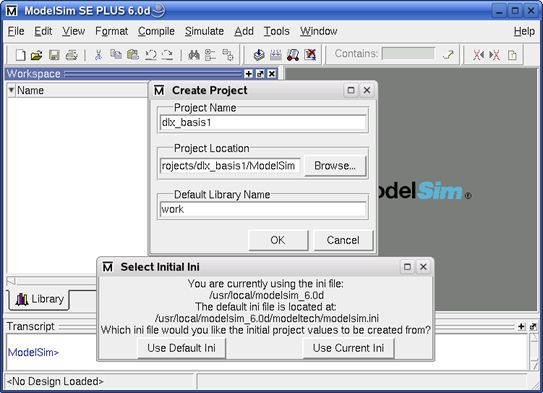
\includegraphics[width=0.9\textwidth]{src/images/5-1.png}
	\caption{Creating a ModelSim Project}
	\label{fig:fig51}
\end{figure}
\begin{figure}[!htb]
	\centering
	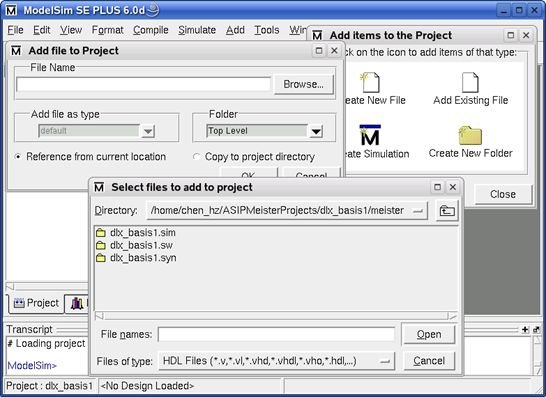
\includegraphics[width=0.9\textwidth]{src/images/5-2.png}
	\caption{Adding Files to a ModelSim Project}
	\label{fig:fig52}
\end{figure}
\hypertarget{adding-the-testbench-and-asip-meister-cpu-files}{%
\subsection{Adding the Testbench and ASIP Meister CPU
files}\label{adding-the-testbench-and-asip-meister-cpu-files}}

Choose the icon ``\emph{Add Existing File''}. Browse to the VHDL netlist
files for the processor e.g. ``\emph{meister/ dlx\_basis1.syn}''
directory of your ASIP Meister project. Here you will find the VHDL
files for synthesis. There is also a VHDL model of the processor in the
\emph{.sim} directory, but do {not} use the files of the \emph{.sim}
directory, as they do not work properly. Select all the files and
confirm the dialog with ``\emph{open}''. Once again, choose the icon
``\emph{Add Existing File''} to add the testbench files:
\emph{tb\_browstd32.vhd}, \emph{MemoryMapperTypes.vhd},
\emph{MemoryMapper.vhd}, and \emph{Helper.vhd} from the \emph{ModelSim}
directory of your current project.

\hypertarget{compile-the-project}{%
\subsection{Compile the project}\label{compile-the-project}}

Menu: Compile \textgreater{} Compile Order \textgreater{} Auto Generate

Every file is compiled and you can see the result of the compile
process. ModelSim determines automatically the compile order of the VHDL
files. After closing the dialog every file should have a green mark
before its name, showing that the compilation was successful (instead of
the question marks), shown in Figure \ref{fig:fig54}. A
green mark with a yellow dot is a warning that usually indicates a
problem. So take care about the warnings.

\textbf{IMPORTANT}: When you edit your CPU in ASIP Meister and execute
\emph{HDL Generation}, then the VHDL files are regenerated and have to
be recompiled. ASIP Meister might even generate new files, that have not
been there in the previous set of VHDL files, e.g. for new pipeline
registers that are needed for modified \emph{MicroOp Descriptions}.
These new VHDL files are not included into your ModelSim project yet.
Also previously needed VHDL files might no longer be needed for a
modified ASIP Meister CPU and ModelSim will complain about these files
while recompiling. To avoid manually checking every VHDL file, whether
it already was included into your project or whether it is a new file,
you can do the following: Delete the \emph{meister/dlx\_basis1.syn}
directory before executing the \emph{HDL Generation}; this will make
sure that no files that are no longer needed exist. Remove all ASIP
Meister VHDL files out of your ModelSim project and after executing the
\emph{HDL Generation} just add the newly created VHDL files from the
\emph{meister/dlx\_basis1.syn} directory, like explained in the previous
paragraph. Instead of the sub window shown in Figure \ref{fig:fig52}, when creating a new project, you
can use the menu: \emph{File \textgreater{} Add to Project
\textgreater{} Existing File}.

\hypertarget{run-the-simulation}{%
\subsection{Run the simulation}\label{run-the-simulation}}

Menu: Simulate \textgreater{} Start Simulation

Open the work library, mark the entry \emph{cfg} (that is the VHDL
configuration for the testbench) in the list (as shown in Figure \ref{fig:fig54}) and press OK. That will start the
simulation and you will get some other window like ``\emph{Objects}'',
``\emph{Processes}'', ``\emph{Wave}'' and a ``\emph{sim}'' tab attached
to the Workspace.

IMPORTANT: Make sure that no \emph{Component Unbound} Message is printed
while starting the simulation. If such a message is printed, then this
is a serious problem within the simulation. Usually it helps to
recompile everything and to start the simulation again (\emph{menu:
Compile \textgreater{} Compile All}). However, a new VHDL file, that was
automatically created by ASIP Meister, but that is not included into
your project yet, can also cause such a message.

Menu: Tools \textgreater{} Tcl \textgreater{} Execute Macro\ldots{}
\begin{figure}[!htb]
	\centering
	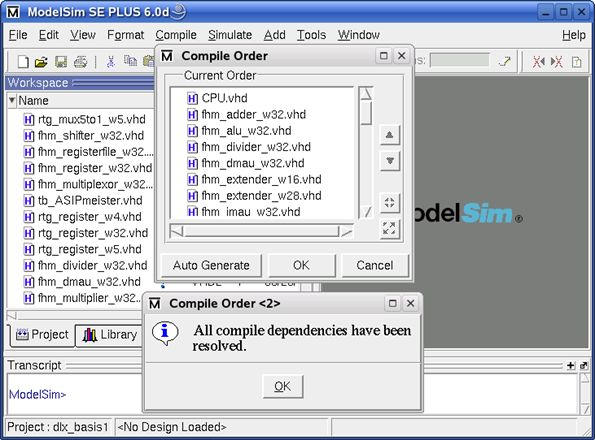
\includegraphics[width=0.9\textwidth]{src/images/5-3.png}
	\caption{Compiling the Project}
	\label{fig:fig53}
\end{figure}
\begin{figure}[!htb]
	\centering
	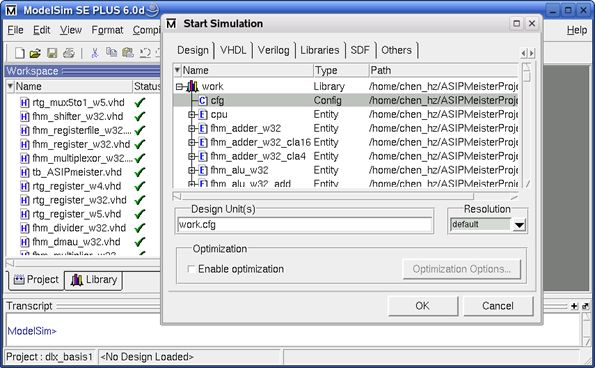
\includegraphics[width=0.9\textwidth]{src/images/5-4.png}
	\caption{Starting the ModelSim Simulation}
	\label{fig:fig54}
\end{figure}
Select the \emph{wave\_vhdl.do} file in your \emph{ModelSim} directory
and press OK to load it. The wave-window will be filled with certain
signals that are useful to evaluate the simulation of the program
running on the processor. These signals are explained in Chapter~5.1.5.

Press the button \emph{Run all} to run the simulation until it aborts.
At the end of a simulation the message ``\emph{Failure: Simulation
End}'' is printed. The type ``\emph{Failure}'' is only used to
automatically abort the simulation. This is not a real failure. At the
simulation end, the file \emph{TestData.OUT} is created in your
\emph{ModelSim} directory. It contains the content of the simulated
memory after the CPU finished working. Therefore, if your algorithm is
storing the result in the memory you can find the values here.

If you want to run another simulation with a modified program or with a
modified initial data memory on the same CPU, then execute again
``\emph{make sim}'' in the respective application subdirectory to create
the new \emph{TestData.IM} and \emph{TestData.DM} and afterwards you
have to press the buttons \emph{restart} and \emph{run all}, like shown
in Figure \ref{fig:fig55}.
\begin{figure}[!htb]
	\centering
	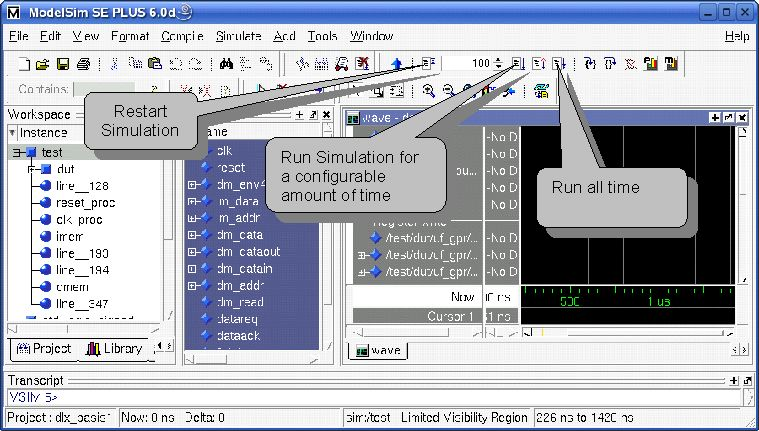
\includegraphics[width=0.9\textwidth]{src/images/5-5.png}
	\caption{Running the ModelSim Simulation}
	\label{fig:fig55}
\end{figure}
\hypertarget{statistics-of-the-simulation}{%
\subsection{Statistics of the
Simulation}\label{statistics-of-the-simulation}}

During simulation time, the testbench prints status messages about
memory access (Load/Store operations) into the workspace status window.
Thus, you can see which operation is being executed and which values are
being stored and loaded. The following examples show a read and a write
access:
\begin{lstlisting}
# ClockCycle:23 InstrAddr:0x00000042 DMemAddr:0x0000FFF0 --> 0 (Read)
# ClockCycle:30 InstrAddr:0x00000049 DMemAddr:0x0000FFF4 <-- 0 (Write 32-Bit) (Old value was 45)
\end{lstlisting}
The read access is performed in cycle 23 while the currently requested
instruction memory address (\emph{IM\_addr\_out}) is 0x42. This does not
mean, that the corresponding load instruction is fetched into the
pipeline in cycle 23 or that this load instruction is placed at
\emph{IM\_addr\_out} 0x42. Instead, this means that the MEM-Phase of the
corresponding load instruction is executed in cycle 23 and that the
instruction at address 0x42 is fetched into the pipeline, while this
load instruction is performing its MEM phase. The corresponding load
instruction is usually placed some instructions before the printed
\emph{IM\_addr\_out}, unless there was a jump in between. The loaded
value is zero in the printed example and this value comes from address
0xFFF0. This is a stack operation, as the stack is starting at address
0xFFFF and growing downwards in our case (but the starting address of
the stack might be a subject of changes). The loaded value is zero in
this example. The afterwards printed write-example additionally shows
which value is placed in the memory location that is to be overwritten.

A more detailed kind of statistics for the simulation is the wave
diagram as shown in Figure \ref{fig:fig56}. The waves
show the internal details of the VHDL model that is simulated. The waves
are grouped into five parts, which are explained in Table \ref{fig:fig57}. For
more details of the memory signals, see Page-47 in \cite{RM}.
\begin{figure}[!htb]
	\centering
	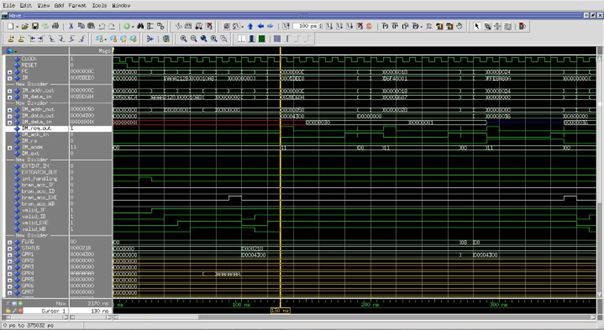
\includegraphics[width=0.9\textwidth]{src/images/5-7.png}
	\caption{ModelSim Waveforms}
	\label{fig:fig56}
\end{figure}
To add additional signal to the Wave window (which is very helpful for
debugging) you need to enable two views in ModelSim (both are enabled by
default):

Menu: View \textgreater{} Workspace

Menu: View \textgreater{} Debug Windows \textgreater{} Objects
\begin{table}[!htb]
	\centering
	\begin{tabular}{|p{4cm}|p{13cm}|}
		\hline
		\multicolumn{1}{|c|}{\textbf{Signal}} & \textbf{Explanation}                                                               \\ \hline
		RESET & The \emph{reset} signal of the CPU. This signal is active at the
		beginning of every simulation to initialize the CPU.\\\hline
		CLOCK & The \emph{clock} signal of the CPU. This signal is helpful to
		see, when other signal changes are really taken into the CPU, as they
		are only sampled at the rising edge of the clock.\\\hline
		PC & Program counter\\\hline
		IR & Instruction register\\\hline
		clock\_counter & The clock counter counts the number of executed clock
		cycles since the CPU started running after the initial
		reset.\\\hline
		IM\_addr\_out & This is the Instruction Memory Address. It shows the
		address of the instruction that the CPU wants to fetch into its
		pipeline.\\\hline
		IM\_data\_in & This is the Instruction Memory Data that corresponds to
		the previous shown \emph{im\_addr}. Therefore, it is the binary
		representation of the assembly instruction that is fetched by the
		CPU.\\\hline
		DM\_addr\_out & This is the Address Bus for memory accesses. This bus
		either contains the address to which some data will be written or the
		address from which some data will be read.\\\hline
		DM\_data\_out & The Data Bus contains the value that will be written to
		the memory.\\\hline
		DM\_data\_in & The Data Bus contains the value that will be read from
		the memory.\\\hline
		DM\_req\_out & This is the request signal from CPU to trigger a read or
		a write access.\\\hline
		DM\_ack\_in & This is the acknowledge signal, that is activated by the
		memory controller after a requested write access is finished or after
		the data bus contains the result of a requested read
		access.\\\hline
		DM\_rw & Read from the memory if 0, otherwise write to the
		memory.\\\hline
		DM\_mode & This signal determines the read/write mode. The usual values
		are ``11'' for ``word'' and ``00'' for ``byte''
		read/write.\\\hline
		DM\_ext & Sign extension signal\\\hline
		EXTINT\_IN, 
		EXTCATCH\_OUT, 
		int\_handling & 
		Interrupt Signals \\\hline
		bran\_acc\_IF,
		bran\_acc\_ID,
		bran\_acc\_EXE,
		bran\_acc\_WB,
		valid\_IF,
		valid\_ID,
		valid\_EXE,
		valid\_WB & 
		Pipeline stages information \\\hline
		FLAG,
		STATUS, 
		GPR1... GPR31 & 
		Register file values \\\hline
	\end{tabular}
	\caption{Explanation of the Signals in the ModelSim Waveform}
	\label{fig:fig57}
\end{table}

In the ``\emph{Workspace}'', you can choose which instance of your
design will be shown in the ``\emph{Objects}'' windows. From the Objects
window, you can then drag-and-drop signals to the Wave window.
\hypertarget{general-hints}{%
\section{General Hints}\label{general-hints}}
\begin{itemize}
\item
  Change to your \emph{ModelSim} directory inside your project directory
  tree and verify that the memory images \emph{TestData.IM} and
  \emph{TestData.DM} are present. The Makefile should have automatically
  created these files. Furthermore, you need the ModelSim testbench file
  \emph{tb\_browstd32.vhd} and the configuration script
  \emph{wave\_vhdl.do}, which are available in the
  \emph{TEMPLATE\_PROJECT/ModelSim} directory. Please make sure that
  these files exist in your \emph{ModelSim} directory before you start
  the simulation. It keeps you safe from trouble.
\item
  Always invoke ModelSim in the specific \emph{ModelSim} directory of
  your current project by executing \emph{vsim \&} in this directory.
  ModelSim is working with project directories and is searching for
  information in the directory where it is invoked. After creating new
  projects all settings will be saved in the project file e.g.
  \emph{projectname.mpf} (where mpf stands for ModelSim Project file).
  To speed up the starting process you can invoke \emph{vsim} with an
  option for your project file that you have created in an earlier
  simulation: ``\emph{vsim projectname.mpf \&''.}
\item
  When you compile VHDL files ModelSim creates a local library in the
  subdirectory \emph{work} to store the compilation results. This is the
  main reason why it is important to start ModelSim in the right place.
  It looks for last project information and for the local library.
\item
  Sometimes you might get compiler errors from the ModelSim VHDL
  compiler. This is usually not the fault of ASIP Meister or the
  testbench. Very often, a ``\emph{recompile all}'' solves this problem.
  However, sometimes you will have to create a new project from the
  scratch to get it working.
\item
  If you open the waves before the simulation is started, then the
  signals will not be displayed. First start the simulation, and then
  open the waves.
\end{itemize}
 
\hypertarget{validating-the-cpu-in-prototyping-hardware}{%
\chapter{Validating the CPU in Prototyping
Hardware}\label{validating-the-cpu-in-prototyping-hardware}}

In this step, we will test the CPU and application, which were generated
in the previous steps, on a FPGA prototyping system. For this purpose,
we will use the XUPV5-LX110T Prototyping Board from Xilinx shown in Figure \ref{fig:fig61}.
\begin{figure}[!htb]
	\centering
	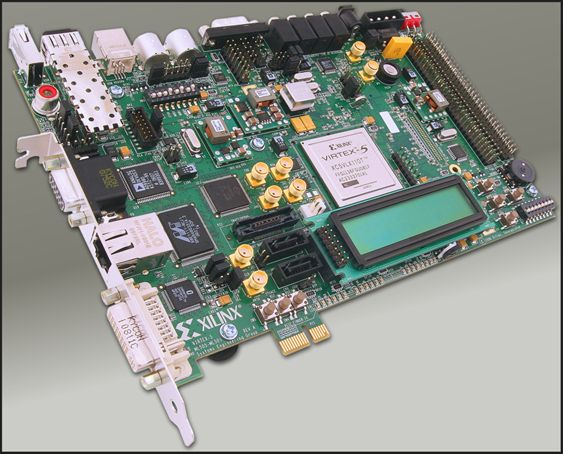
\includegraphics[width=0.9\textwidth]{src/images/6-1.png}
	\caption{XUPV5-LX110T Prototyping Board from Xilinx \cite{HWAFX}}
	\label{fig:fig61}
\end{figure}
\hypertarget{creating-the-ise-project}{%
\section{Creating the ISE Project}\label{creating-the-ise-project}}

ISE (also called Project Navigator) is a program from Xilinx to support
the whole tool-flow from managing your source files during synthesis,
map, and place \& route until finally uploading the design to the FPGA
board.

Start ISE by just executing ``\emph{ise \&''} in your ASIP project
directory

If you do not already have a project for your current CPU, then create a
new one: Select \emph{File} Menu \textgreater{} \emph{New~Project}. As
``\emph{Project Path''} you should choose your ASIP Meister Project
Directory (e.g. ``\emph{ASIPMeisterProjects/browstd32/'')} and as
``\emph{Project Name''} you can choose something like
``\emph{ISE\_Framework}''. This ``\emph{Project Name''} will then
automatically be added as new subdirectory to your chosen \emph{Project
Directory}. In the upcoming window ``\emph{Device Properties}'', you
have to adjust the values to the data shown in Figure \ref{fig:fig62}. Afterwards just press \emph{Next
\textgreater{} Next \textgreater{} Finish} to create an empty project
for your CPU. The device settings are needed to make sure, that the map,
place and route tools know exactly the type of the target FPGA. For
example, you will have a project with following project settings:
\begin{lstlisting}
Project Name: ISE_Framework
Project Path: home/asip04/ASIPMeisterProjects/browstd32/ISE_Framework
Device Family: Virtex5
Device: xc5vlx110t
Package: ff1136
\end{lstlisting}
\begin{figure}[!htb]
	\centering
	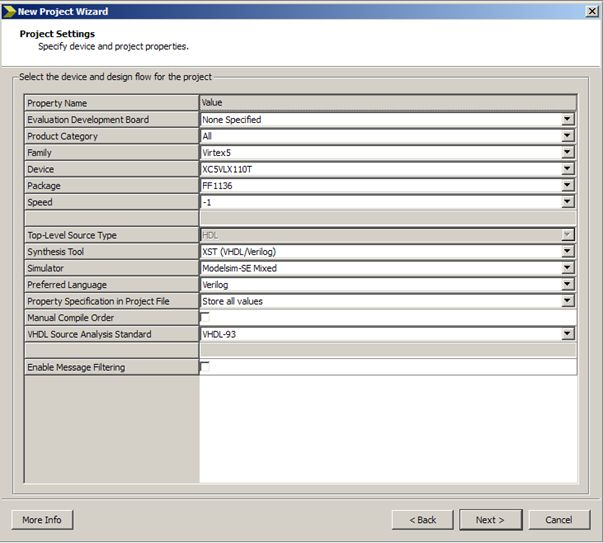
\includegraphics[width=0.9\textwidth]{src/images/6-2.png}
	\caption{ISE Device Properties}
	\label{fig:fig62}
\end{figure}
\hypertarget{adding-source-files-to-ise-project}{%
\section{Adding Source Files to ISE
Project}\label{adding-source-files-to-ise-project}}

Now you have to add the needed VHDL and constraint files to your ISE
project, by right clicking on the XC5VLX110T-1ff1136 entry of your
Sources View (at the upper left inside your ISE Window, see Figure \ref{fig:fig63} \&
Figure \ref{fig:fig64}) and choosing ``\emph{Add Copy of
Source}''. After ISE has analyzed the type of the files, press OK.
Adding a copy of the source has the advantage, that you can locally
modify the files and that the CPU files in your ISE project are not
overwritten, when you modify your ASIP Meister Project for testing
purpose.

There are three types of files that are needed for a hardware
implementation:

\begin{itemize}
\item
  CPU VHDL Files
\item
  Framework Files
\item
  Framework IP cores
\end{itemize}
\begin{figure}[!htb]
	\centering
	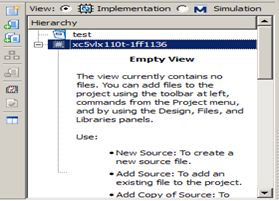
\includegraphics[width=0.7\textwidth]{src/images/6-3.png}
	\caption{Add Sources}
	\label{fig:fig63}
\end{figure}
\begin{figure}[!htb]
	\centering
	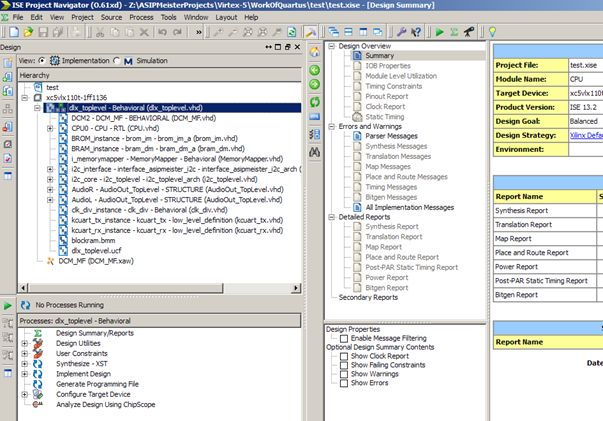
\includegraphics[width=0.9\textwidth]{src/images/6-4.png}
	\caption{ISE Project Overview}
	\label{fig:fig64}
\end{figure}
\textbf{CPU VHDL Files} have been generated using ASIP Meister and they
can be found in the \emph{meister/\{CPU-Name\}.syn} directory, as
explained in Chapter~2.2.2.

\textbf{Framework Files} are important for the connection between CPU,
Memory, UART, and all other components. They are predesigned for this
laboratory and they are available in
\emph{/homeasip00/­ASIPMeisterProjects/­TEMPLATE\_PROJECT/­ISE\_Framework}.
The framework consists of the following three types of file and all of
them have to be added to the ISE project.

\begin{itemize}
\item
  \begin{quote}
  The VHDL files describe how all components are connected together.
  \end{quote}
\item
  \begin{quote}
  The UCF file describes the user constraints (e.g., which I/O pins
  should be used for a signal, which clock frequency is requested etc.).
  \end{quote}
\item
  \begin{quote}
  The BMM file contains a description of the memory buildup for
  instruction- and data-memory for the CPU. Out of this file
  \emph{\ldots\_bd.bmm} file will be generated while implementation and
  this file is then used to initialize the created bitstream with the
  application data, as explained in Chapter~6.4.
  \end{quote}
\end{itemize}

\textbf{IP cores} are used within the framework, e.g. memory blocks for
instruction- and data-memory or FIFOs for the connection to the LCD.
These IP cores are not available as VHDL source code, but instead they
are available as pre-synthesized net lists. These files just have to be
copied into the directory of your ISE project (no need to actually add
them to the project) and then they will be used during the
implementation step. The needed files (*.edn, *.ngc) are available in
\emph{/home/asip00/­ASIPMeisterProjects/­TEMPLATE\_PROJECT/­ISE\_Framework/­IP\_­Cores}.
Note: The files {inside} the IP\_Cores directory have to be copied to
your ISE Project Directory. It is not sufficient to copy the full
IP\_Cores directory!

After you have added/copied all needed files to your ISE
project/directory, your main window should look similar to the
screenshot shown in Figure \ref{fig:fig64}. In the
sources sub window you can see all the source files and how they are
structured, i.e. according to the file instantiated by other file.

\hypertarget{synthesizing-and-implementing-the-ise-project}{%
\section{Synthesizing and Implementing the ISE
Project}\label{synthesizing-and-implementing-the-ise-project}}

In the Processes sub window in the lower left corner of
Figure \ref{fig:fig64}, the possible actions for each
kind of file is shown. To synthesize and to implement your project you
have to choose your VHDL-Toplevel in the Sources sub window
(``\emph{dlx\_Toplevel}'' in the figure) and afterwards you have to
double click ``\emph{Generate Programming File}'' in the Processes sub
window. This will finally create the .bit file that can then be
initialized with your CPU instruction- and data-memory and afterwards be
uploaded to the FPGA prototyping board.

The whole process of synthesizing and implementing the design is
subdivided into several steps that can be seen, if you click on the plus
sign in the processes sub window. After the completion of each step, an
update of the \emph{FPGA Design Summary} will be shown in the
corresponding sub window in the upper right corner. For example, the
device utilization (i.e. the size of your CPU plus the framework) will
be shown for the different types of elementary hardware available on the
FPGA (e.g. clocks, logic, BRAMs). This is a first hint, how big your CPU
actually is, but as it will be explained in Chapter~6.5, these values
are not completely accurate, as they not only include the CPU, but also
include the Framework, which consists of many different components.

While synthesizing and implementing the design, many warnings will be
printed. These warnings (unless created by a user modification, e.g. in
the CPU) can be ignored. However, it should be mentioned, that it is
very helpful to understand the meaning of these warnings when you are
looking for a reason why something is working unexpected in hardware.
The challenge here is, that the CPU and the IP cores create plenty of
warnings, thus it is hard to locate the serious warnings.

\hypertarget{initializing-fpga-internal-memory-with-your-application}{%
\section{Initializing FPGA Internal Memory with your
Application}\label{initializing-fpga-internal-memory-with-your-application}}

After you have finished the synthesizing and implementation step, you
receive a bitstream of your ISE project that includes your CPU connected
to an internal memory inside the FPGA. Now you have to initialize this
FPGA internal memory (called Block RAM or BRAM) with your application
instruction- and data memory to execute your program on your CPU. This
initialization can be done inside the bitstream itself, i.e. before
uploading the bitstream to the FPGA board.

To initialize the bitstream with your application, you need your
application as \emph{TestData.IM} and \emph{TestData.DM} files, created
with ``\emph{make sim}'' or ``\emph{make dlxsim}'' as explained in
Chapter~2.3. However, compared to simulation with dlxsim or ModelSim you
have to consider, that you have a limited amount of memory on the FPGA
and therefore you have to adjust the position were the stack starts. For
the usual simulation, the stack can start at some address e.g, 0xFFFFC
and is growing downwards. For hardware execution, this address is too
big. For the current hardware prototype, you should use 0xEFFC. You can
adjust the place where the stack will start in the file
\emph{/home/asip00/epp/mkimg/Makefile} by adjusting
\emph{STACK\_START\_FPGA} variable. This \emph{Makefile} is accessed
from your local application \emph{Makefile} located in the directory of
your application (like
\emph{/home/asip00/­ASIPMeisterProjects/­TEMPLATE\_PROJECT/­Applications/­TestPrint/Makefile})
and it is evaluated every time you execute this local \emph{Makefile}.
Here you can configure the address of the stack start. To work in
hardware this value depends of the size of the available memory in
hardware. For our current prototype, ``0xEFFC'' is the correct value. In
case of FPGA, this parameters is set to STACK\_START\_FPGA.

After the \emph{TestData}-files for your application are created (see
above and Chapter~2.3) and the bitstream of your ISE project is created
(see Chapter~6.1 and Chapter~6.3) you can initialize the bitstream with
your application data by executing ``\emph{make fpga}'' in your
application subdirectory. This script will create two new files in
\emph{BUILD\_SIM} subdirectory of your application like
\emph{DirectoryName.mem} and \emph{DirectoryName.bit}. The .mem file
contains a memory dump for data and instruction memory and is only a
temporary file. The bit file is the final bitstream of your specific CPU
surrounded by the framework, and with your application initialized to
the BRAM. You have to configure the ISE project that you want to use in
the ``\emph{env\_settings}'' as ``\emph{ISE\_NAME}''. The bitstream in
this directory will be used to create the application-initialized
bitstream.

\hypertarget{uploading-the-bitstream-to-fpga-board}{%
\subsection{Uploading the Bitstream to FPGA
Board}\label{uploading-the-bitstream-to-fpga-board}}

After you have created the final bitstream with the initialized BRAM,
you can upload this bitstream to the FPGA Board. At first, you have to
turn the FPGA Board on.
\begin{figure}[!htb]
	\centering
	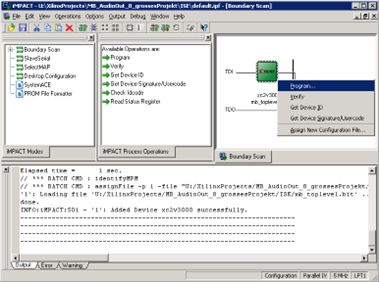
\includegraphics[width=0.9\textwidth]{src/images/6-5.png}
	\caption{Uploading the Bitstream with iMPACT}
	\label{fig:fig65}
\end{figure}
After the FPGA Board is running, you have to connect the FPGA to the PC
and then initialize it with your Bitstream. Therefore, the software
iMPACT from Xilinx, shown in Figure 6-5 is used. If you try to start
iMPACT you will receive an error message, complaining about the
project-/ and the working directory (because you are not an
administrator on this PC). Therefore, right-click the symbol and choose
``\emph{properties}''. Then configure the working directory to
``\emph{U:}'' (this is your mounted Linux-server home). Afterwards you
can start iMPACT. Create a new project (no need to `save' and `load' a
project) and choose the default point ``\emph{Configure Device using
Boundary Scan (JTAG)}''. You should see a JTAG chain with one device
(the FPGA) as shown in Figure 6-5. Assign the bitstream of your
application subdirectory
(ASIPMeisterProjects/browstd32/Applications/...) to the Xilinx FPGA
device. To reactivate this menu point in a later run without restarting
iMPACT, just right-click on the Xilinx device and choose ``\emph{Assign
New Configuration File}''. To program the Xilinx device (i.e. the FPGA)
choose ``\emph{Program}'' as shown in Figure 6-5 and confirm the dialog
without any changes with ``OK''.

Instead of using graphical iMPACT tool for uploading the bitstream to
the FPGA, you can use your Makefile ``\emph{make upload}'' in your
application subdirectory to upload the combined bitstream to the FPGA.
This will automatically scan and program the FPGA.

\hypertarget{initializing-and-using-the-external-sram}{%
\subsection{Initializing and Using the External
SRAM}\label{initializing-and-using-the-external-sram}}

The size of the BlockRAM (i.e. FPGA-internal RAM; at most 192 Kbyte for
our FPGA, but something is used in the Framework for FIFOs etc.) is
limited. This is especially problematic if a huge amount of input-data
is to be used for an application. Therefore, we have provided external
SRAM to the Board, altogether four MB SRAM for IM and four MB SRAM for
DM respectively. Our provided ISE Framework (see Chapter~6.1) provides
the connection between the CPU and the SRAM. However, before the SRAM
can be used it has to be initialized. Currently the SRAM initialization
is unexpected slow. Therefore, whatever you want to test on the FPGA
board, test a BlockRAM version first. The provided ISE Framework still
provides the connection to the BlockRAM additionally. You just have to
follow the above tutorials (Chapter~6.4 and 6.4.1) but do not forget to
configure \emph{STACK\_START\_FPGA} in the Makefile to 0xEFFC. To use
the SRAM, follow the following tutorial:

\begin{itemize}
\item
  You have to compile the \emph{bootloader.c} application (you can find
  it in
  \emph{/home/asip00/­ASIPMeisterProjects/­TEMPLATE\_PROJECT/­Applications/­Bootloader/})
  with ``\emph{make sim}'' and initialize the bitstream with the
  application using ``\emph{make fpga}''. The resulting bit file
  contains the bootloader application in the FPGA internal BlockRAM.
\item
  You have to compile the user application (i.e. the one that you
  actually want to run from the SRAM) with the \emph{STACK\_START\_FPGA}
  configured to 0xFFFFC (in the Makefile; instead of 0xEFFC for BRAM).
  Note that, besides the normal \emph{TestData.IM} and
  \emph{TestData.DM} additionally the files \emph{TestData.IM\_uart.txt}
  and \emph{TestData.DM\_uart.txt} are also created in the
  \emph{BUILD\_SIM} subdirectory.
\item
  You have to start the ``\emph{dlx\_uart.ht}'' file under windows,
  which will open the MS Windows HyperTerminal with the correct settings
  (\emph{Bits per Second=230400, Data Bits=8, Parity=None, Stop Bit=1,
  Flow Control=None}). You can find ``\emph{dlx\_uart.ht}'' in
  \emph{/home/asip00/­ASIPMeisterProjects/­TEMPLATE\_PROJECT/­Applications/­Bootloader}).
  However, you may have to adapt the configured COM port, depending on
  which port you are connected to the FPGA (see
 Figure \ref{fig:fig66}). Under, Ubuntu, you can start
  HyperTerminal by typing ``\emph{hterm \&}'' and can configure the
  settings as mentioned before. After that, you have to click the
  ``\emph{connect}'' button to open the connection. Opening the
  connection always works without error message, but you have to make
  sure that the FPGA board is connected to the PC where you are running
  the HyperTerminal via UART.
\item
  Now configure the FPGA Board to run with 40 MHz (see point (9) in
  Figure \ref{fig:fig66}) and upload the bootloader
  bit-file (created in first step) with iMPACT. The UART port on the
  FPGA is configured to work with 40 MHz and if you use a faster or
  slower frequency, then you will not see the correct output via UART.
  The bootloader will prompt on the UART-Console for initializing the
  SRAM. It will ask for three things (you have to answer with pressing
  `y' or `n'): Initialize IM, Initialize DM, and Start Application.
\item
  To initialize IM or DM you have to select `y' and then use the
  HyperTerminal menu ``\emph{Übertragung}'' ``\emph{Textdatei senden}''
  to upload the file \emph{TestData.IM\_uart} or
  \emph{TestData.DM\_uart}.
\item
  If you do not start the application in the IM-SRAM (pressing `n' when
  asked) OR when the IM-SRAM application is finished OR when you press
  the reset button THEN you will come back to the bootloader.
\end{itemize}
\begin{figure}[!htb]
	\centering
	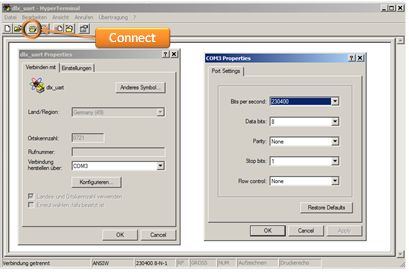
\includegraphics[width=0.7\textwidth]{src/images/6-6.png}
	\caption{Hyper-terminal settings}
	\label{fig:fig66}
\end{figure}
\hypertarget{hardware-specific-limitations-of-the-application}{%
\subsection{Hardware Specific Limitations of the
Application}\label{hardware-specific-limitations-of-the-application}}

Many kinds of applications can be simulated with dlxsim or ModelSim, but
to be able to be executed in hardware, there are some further
limitations, which have to be considered. The most obvious point is the
limitation of the available memory for instructions and data on the
hardware prototype. Currently there are 16 KB for instruction and 16 KB
for data memory available. A part of the ``\emph{make fpga}'' script
will test, whether the your application binary including program and
static data memory fits into these memory portions, but for dynamic
requested data memory, like the stack which is growing with the number
of nested function calls cannot be tested at compile time. If you need
more memory, you have to use the SRAM instead (see Chapter~6.4.2).

Another point is that there are more NOP instructions needed for
hardware execution than for simulation. Therefore, ``Makefile'' file has
to be adjusted accordingly as explained in Chapter~6.4.

The current connection to the data memory does only support word access
to the data memory. Thus, the only supported memory access assembly
instructions are ``\emph{lw}'' and ``\emph{sw}''. The assembly
instructions ``\emph{lb}'', ``\emph{lbu}'', ``\emph{lh}'',
``\emph{lhu}'' actually work as well, because they load a full word from
the memory and extract the required part of it inside the CPU. However,
the instructions ``\emph{sb}'' (store byte) and ``\emph{sh}'' (store
half word) will not work in the current hardware prototype and thus have
to be avoided! A part inside the ``\emph{Makefile}'' script will test,
whether some of these unsupported instructions are used and it will
generate a warning that this application will not run in the current
hardware prototype (though it works fine in dlxsim and ModelSim). As a
workaround for accessing bytes (e.g. for string to be printed on the
LCD) some special functions are provided in the StdLib directory (see
Chapter~8.3).
\begin{lstlisting}
int storeByte(char* address, int value);
int storeShort(char* address, int value);	
\end{lstlisting}


With these functions, you can indirectly access specific bytes and
half-words by only using ``\emph{lw}'' and ``\emph{sw}'' assembly
instructions.

\hypertarget{getting-accurate-area-delay-and-critical-path-reports}{%
\section{Getting Accurate Area, Delay and Critical Path
Reports}\label{getting-accurate-area-delay-and-critical-path-reports}}

The results for area and speed for your synthesis result like created
with the tutorial in Chapter~6.1 are not accurate. This is, because the
provided framework contains extra additions like a state machine to
communicate with the LCD via the I\textsuperscript{2}C bus or the data-
and instruction memory and its connection to the CPU. These additions,
which are needed for running the CPU on the hardware prototype, have a
big impact on the measured size and speed of your CPU. Therefore, if you
try to compare two different CPUs with the provided framework, you will
mainly compare the framework with itself and it is hard to separate,
which change in e.g. the CPU frequency is due to a change in the CPU or
a more efficient optimization of the synthesis program due to a better
interaction of CPU and framework.

To come around the above-mentioned problems, one might suggest
synthesizing the plain CPU without any kind of framework to get accurate
data without any impact of other components. Nevertheless, when you look
at the output of this synthesis, you will notice, that all internal
connections of the CPU will be automatically mapped to I/O-Pins of the
FPGA, which has an impact of the size and speed of the synthesis result
as well. This impact is due to the fact, that the I/O pins are rather
slow compared to the FPGA-internal computation. However, you cannot
force the synthesis tools to let the CPU connections unconnected,
because then the synthesis tool would notice that there is no input to
the CPU and that the output of the CPU is not used at all and thus it
would remove the whole CPU for optimization reasons.

The above two examples will give you an impression how difficult it is
to measure your results and how difficult it is to interpret the results
of your measurements or even more: to compare two different measurements
with each other. However, first we have to understand the unit in which
the area is measured for FPGAs, i.e. a \emph{Slice}.

The basic block of a fine-grained configurable hardware as in FPGAs is a
Look-Up-Table (LUT) as shown in Figure \ref{fig:fig69}.
The shown example (use four inputs at the top and 1 output at the right
side) can realize every Boolean function with four inputs. For each
input combination (2\textsuperscript{4}=16), a dedicated configuration
bit (S0-S15) can be programmed with the corresponding answer. The
transistors feed the value of the selected configuration bit to the
output. For instance, if S0-S14 are programmed to contain the value `0'
and just S15 is programmed to contain the value `1', then this LUT
behaves like a 4-input AND-gate.

Many of the 4-LUTs are required, for example, to implement a 32-bit
adder and additionally these LUTs have to be connected. FPGAs typically
cluster their logic, i.e. they have local blocks with a strong
interconnect, but less strong global interconnects.
Figure \ref{fig:fig610} shows how Xilinx clusters the
LUTs into so-called Slices (including a 1-bit register per LUT) and
Configurable Logic Blocks. They have strong interconnects and especial
logic for e.g. carry-chains to implement adders.
Figure \ref{fig:fig611} shows how the CLBs are connected
with configurable switches and dedicated connections.

Altogether, FPGAs provide a huge amount of these logic resources, e.g.
the Virtex-II 3000 offers 14,336 Slices. The biggest Virtex-II FPGA
(i.e. 8000) offers 46,592 Slices and the biggest Virtex-5 FPGA even
offers 51,840 Slices (note: Virtex-5 additionally offers more logic per
slice). Additionally they offer dedicated IP cores, e.g. multi-standard
I/O ports, Digital Clock Managers, BlockRAMs, multipliers, and even
PowerPC cores.
\begin{figure}[!htb]
	\centering
	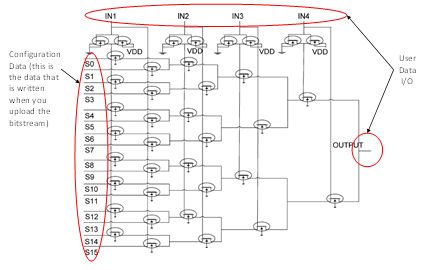
\includegraphics[width=0.8\textwidth]{src/images/6-7.png}
	\caption{4-Input 1-Output Look-Up Table (4-LUT) \cite{Kalenteridis04}}
	\label{fig:fig67}
\end{figure}
\begin{figure}[!htb]
	\centering
	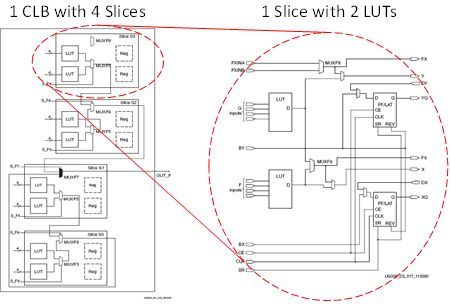
\includegraphics[width=0.8\textwidth]{src/images/6-8.png}
	\caption{CLBs, Slices, and LUTs in a Virtex II FPGA \cite{XUG002}}
	\label{fig:fig68}
\end{figure}
\begin{figure}[!htb]
	\centering
	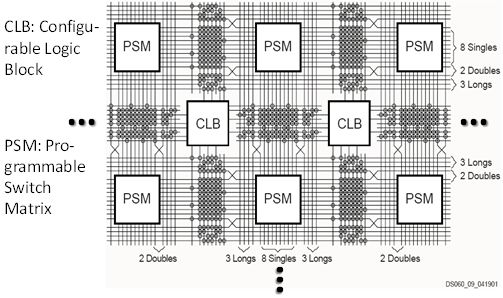
\includegraphics[width=0.8\textwidth]{src/images/6-9.png}
	\caption{ Array of CLBs and PSMs \cite{XDS060}}
	\label{fig:fig69}
\end{figure}
\hypertarget{creating-ise-project-for-getting-accurate-reports}{%
\subsection{Creating ISE Project for Getting Accurate
Reports}\label{creating-ise-project-for-getting-accurate-reports}}

To measure the area and delay of your CPU accurately we designed a new
framework \emph{ISE\_Benchmark}, which consists of four files:
\emph{bram\_dm.ngc}, \emph{brom\_im.ngc}, \emph{dlx\_toplevel.vhd}, and
\emph{dlx\_toplevel.ucf}, which can be found in the directory
``\emph{/home/asip00/­ASIPMeisterProjects/­TEMPLATE\_PROJECT/­ISE\_­Benchmark/}''.
The first two files are BlockRAM netlist files for data and instruction
memories. The VHDL file is the top level for the whole project. The UCF
file is the file, which contains the timing constraints and pins
location for the design (in this step, we specify only the clock and
reset constraints).

Using this framework, all the CPU connections will be mapped to the
FPGA-internal BRAM memory and this will decrease the area needed to
implement the project and will give more accuracy to compute the
processor area and speed. To obtain the area and speed results for your
CPU, your CPU files with this special framework have to be synthesized
and implemented as explained in Chapter~6.1 and Chapter~6.3.

\hypertarget{getting-area-report}{%
\subsection{Getting Area Report}\label{getting-area-report}}

In the Process sub window, expand ``\emph{Place \& Route}'' process.
Double clicking on ``\emph{Place \& Route Report}'' will open new window
containing the results needed. Try to find the number of slices in the
``\emph{Device Utilization Summary}'' as shown in
Figure \ref{fig:fig610}.

\hypertarget{getting-delay-report}{%
\subsection{Getting Delay Report}\label{getting-delay-report}}

In the Process sub window, expand ``\emph{Place \& Route}'' process and
expand ``\emph{Generate Post-Place \& Route Static Timing Report}''.
Double clicking on ``\emph{Text-based Post-Place \& Route Static Timing
Report}'' will open new window containing the results needed. Try to
find minimum Period in the ``\emph{Design Statistics}'' as shown in
Figure \ref{fig:fig611}.
\begin{figure}[!htb]
	\centering
	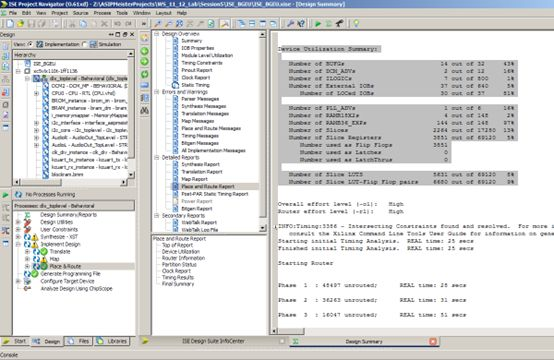
\includegraphics[width=0.9\textwidth]{src/images/6-10.png}
	\caption{Area Report}
	\label{fig:fig610}
\end{figure}
\begin{figure}[!htb]
	\centering
	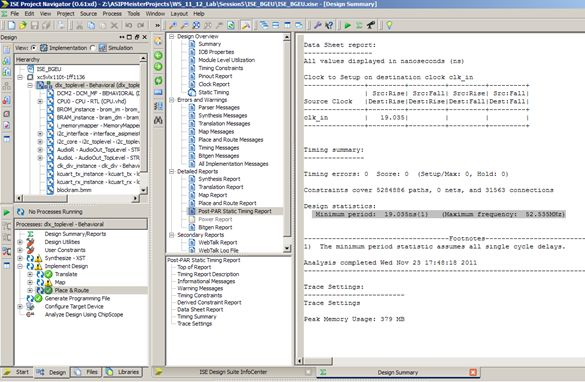
\includegraphics[width=0.9\textwidth]{src/images/6-11.png}
	\caption{Delay Report}
	\label{fig:fig611}
\end{figure}
\hypertarget{getting-critical-path-report}{%
\subsection{Getting Critical Path
Report}\label{getting-critical-path-report}}

To get the critical path, you have to analyze against the timing
constraints. To do that, expand the ``\emph{Place \& Route}'' process in
the sub window \emph{Process}, and then expand ``\emph{Generate
Post-Place \& Route Static Timing Report}''. A double click on
``\emph{Analyze Post-Place\& Route Static Timing (Timing Analyzer)}''
will open a new window for analyzing the timing. In this window, click
on ``\emph{Analyze Analyze against timing constraints}'' as shown in
Figure \ref{fig:fig612}.
\begin{figure}[!htb]
	\centering
	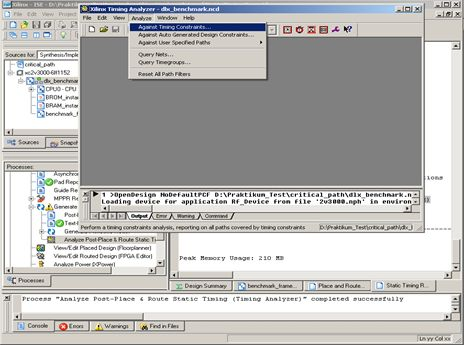
\includegraphics[width=0.9\textwidth]{src/images/6-12.png}
	\caption{Timing Analyzer Window}
	\label{fig:fig612}
\end{figure}
\begin{figure}[!htb]
	\centering
	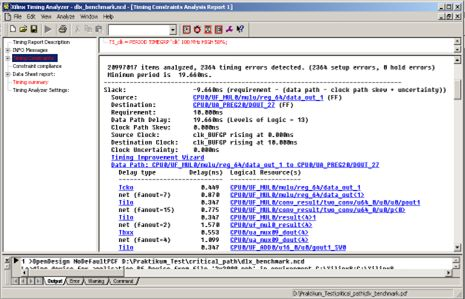
\includegraphics[width=0.9\textwidth]{src/images/6-13.png}
	\caption{Critical Path in the Xilinx Timing Analyzer}
	\label{fig:fig613}
\end{figure}

In the ``\emph{Analyze against timing constraints}'' window, keep
everything as it is and click OK. After a while, the ``\emph{Timing
Analyzer}'' window will be opened. In this window (shown in
Figure \ref{fig:fig613}), click on the ``\emph{Timing
constraint}'' and you will get the critical paths ordered from the
longest to the shorter paths. For each path, you will find the total
delay and the sub-delays for the signals this path consists of.

In the shown example of Figure \ref{fig:fig613}, you can
see, that the path has it's ``\emph{source}'' and ``\emph{destination}''
inside the \emph{CPU0} (i.e. the instantiation of the ASIP Meister CPU,
as it is named in the dlx\_toplevel.vhd). When looking at the detailed
signals this path consists of, you can see, that it starts in the
multiplier of the CPU (MUL0, as it is named in the ``\emph{Resource
Declaration}'' in ASIP Meister), afterwards goes through a multiplexer
(mux09) and then goes to the adder (ADD0, as it is named in the
``\emph{Resource Declaration}'' in ASIP Meister).

When comparing the maximal frequency of two different CPUs you have to
look at the critical paths of both CPUs to understand why maybe the one
CPU is slower than the other or vice versa.
 
\hypertarget{power-estimation}{%
\chapter{Power Estimation}\label{power-estimation}}

In this tutorial we will learn how to estimate the power by using
ModelSim to generate the switching activity of the design, and XPower
(from Xilinx) to analyze the results and generate the final power report
and CosmosScope to visualize the results.

\hypertarget{different-types-of-power}{%
\section{Different Types of Power}\label{different-types-of-power}}

Typically, power dissipation in a cell is subdivided into two different
groups, dynamic power, and static power. \textbf{Dynamic power} is the
power dissipated in a cell when the input voltage is actively
transitioning. Dynamic power is further subdivided into two components
switching power and internal power. \textbf{Switching power} is the
power required to charge the capacitive load on the output pins of the
cell. Switching power is shown in Figure \ref{fig:fig71},
as the I\textsubscript{sw} switching current charging up the
C\textsubscript{load} capacitor. This component of power is calculated
using the familiar ½ CV\textsuperscript{2} equation.

For switching power, all we need to know is V\textsubscript{dd} and the
capacitive load that is driven by the cell. Therefore, the library does
not need to be characterized for this component of power dissipation.
\begin{figure}[!htb]
	\centering
	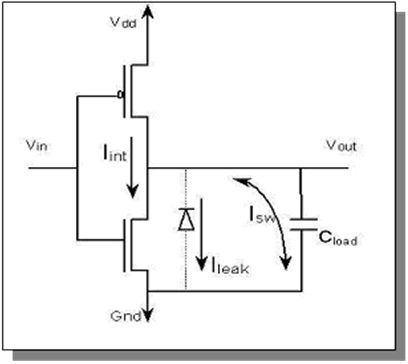
\includegraphics[width=0.7\textwidth]{src/images/7-1.png}
	\caption{Switching Power Dissipation}
	\label{fig:fig71}
\end{figure}
\textbf{Internal power} consists of short-circuit power and power
dissipated by charging the capacitive loads that are internal to the
cell (not shown in the above circuit). Short-circuit power is the power
that is dissipated due to the short period that paths in the cell are
essentially short circuits. In the circuit shown above,
I\textsubscript{int}, that is the current path when the device is
short-circuited, shows internal power. Every time the input
V\textsubscript{in} toggles, there is a short period of time where both
transistors are turned on and there is a path from V\textsubscript{dd}
to ground. The longer both transistors are active, the higher the power
dissipation. The circuit above is quite simple (an inverter) and there
is only one path from V\textsubscript{dd} to ground. For complex
circuits, you could have dozens of potential short circuit paths.
Internal power is dependent on the transition time of the input voltage
V\textsubscript{in} and the output capacitive load. These factors
determine how long the short circuit is active. There is no easy formula
to determine the power dissipated due to internal power, so the cell
must be characterized for it.

\begin{quote}
The final component of power analysis is the \textbf{Leakage power}. In
the circuit diagram in Figure 7-1, it is shown as leak current. This is
the power dissipated when the circuit is in a steady state and it is due
to the following factors inherent in transistors: reverse bias leakage
current, sub-threshold current, or other second-order leakage power.
Leakage power has become a major factor in power analysis in recent era.
\end{quote}

At 180 nm and above, leakage power was typically less than 1\% of the
total power dissipation in a circuit. With 130 nm and below, the leakage
power becomes a much larger factor, up to 50\% of dissipated power in
some cases. Leakage power should be characterized for each cell in the
library.

To report the switching power, we need the switching activities of the
design. The switching activity contains information about the static
probability and toggle rate. The static probability can be calculated
during a simulation by comparing the time a signal is at a certain logic
state (state 0 or state 1) to the total time of simulation. The toggle
rate is the number of transitions between logic-0 and logic-1 (or vice
versa) of a design object per unit of time.

The previous power definitions can be concluded by these two equations:
\begin{lstlisting}
Total Power = Dynamic power + Leakage power
Dynamic Power = Switching power + Internal power	
\end{lstlisting}
\hypertarget{estimating-the-power-consumption}{%
\section{Estimating the Power
Consumption}\label{estimating-the-power-consumption}}

To estimate the power consumption for a specific application on a
specific CPU you need to generate the switching activities, which are
saved as a Value Change Dump (VCD) file. This file is generated when the
project is simulated using ModelSim and the application is executed on
the CPU. Then the VCD file will be used as input to the XPower tool,
which finally will generate the power report. This report can be
visualized using the CosmosScope visualization tool.

\hypertarget{generate-the-vcd-file-using-modelsim}{%
\subsection{Generate the VCD file using
ModelSim}\label{generate-the-vcd-file-using-modelsim}}

The VCD (Value Change Dump) file can be generated during the ModelSim
simulation to capture signals switching activities as explained below:

\begin{enumerate}
\def\labelenumi{(\arabic{enumi})}
\item
  Create a ModelSim project in your project's \emph{ModelSim} directory,
  add your CPU VHDL files from your project's ``\emph{meister/*.syn}''
  directory, and add testbench files from the \emph{ModelSim} directory,
  as explained in the Chapter. Remember that you should already have
  generated \emph{TestData.IM} and \emph{TestData.DM} files in your
  \emph{ModelSim} directory using ``\emph{make sim}''.
\item
  Configure the CPU Frequency for which you want to run the power
  estimation. Open the ModelSim testbench (\emph{tb\_browstd32.vhd}),
  search for CLK\_PERIOD, and change the value accordingly. Take care:
  For simulation-reasons this value corresponds to the time (in
  nanoseconds) of a half clock period. For example, 10 ns half period
  correspond to 20 ns clock period, which is 50 MHz frequency.
\item
  Compile the project Compile Compile Order Auto Generate
\item
  Start the simulation: VSIM \textgreater{} \textbf{vsim -t 1ns
  work.cfg}
\item
  Store the switching activities during the program execution in the VCD
  file e.g. ``\emph{test.vcd}'' by typing: VSIM \textgreater{}
  \textbf{vcd file test.vcd}
\item
  Add all signals of the CPU instance: VSIM \textgreater{} \textbf{vcd
  add -r test/dut/*}
\item
  The entity name of the tutorial example testbench is \emph{test} and
  the instance name of the device under test is \emph{dut}. Using the
  \emph{-r} switch with ModelSim ``\emph{vcd add}'' command will result
  in a large but significantly more accurate VCD file. VCD files can
  grow quite large for larger designs or even for smaller designs if the
  simulation time is long.
\item
  Run the simulation: VSIM \textgreater{} \textbf{run -all}
\item
  The switching activities will be saved in ``test.vcd'' file.
\end{enumerate}

\hypertarget{generating-the-power-report-using-xpower}{%
\subsection{Generating the Power Report Using
xPower}\label{generating-the-power-report-using-xpower}}

The second step is to create an ISE project that you want to analyze for
power consumption. Create a new project and add only the CPU files from
the ASIP Meister ``\emph{meister/xxx.syn}'' directory to it. In the
``\emph{Processes}''-tree of your top-level design and under
``\emph{Implement Design/Place \& Route}'', click on ``\emph{Analyze
Power Distribution (xPower Analyzer)}''. This will open the xPower
window. Now, click on ``\emph{File\textgreater open Design}'', in the
``\emph{Design}'' file, you have to add your .ncd file e.g.
toplevel.ncd'' and in ``\emph{Simulation Activity}'' file, you have to
add the .vcd file that you generated in the previous step. Finally, in
the ``\emph{Physical Constraint}'' file, you can add the .pcf file for
you project e.g. ``toplevel.pcf'' as shown in Figure \ref{fig:fig72}. As soon as you click OK, the
XPower tool will analyze the files and gives you a summary about the
power consumption in your design (like the Leakage power and the total
power). On the right side, you find ``By Clock Domain''. Here you see
the frequency in (MHz). The clock frequency should be the same frequency
that you used in testbench during VCD file generated as shown in Figure \ref{fig:fig73}.
\begin{figure}[!htb]
	\centering
	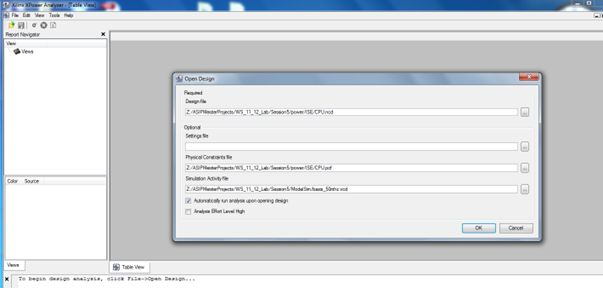
\includegraphics[width=0.9\textwidth]{src/images/7-2.png}
	\caption{Preparing xPower Tool}
	\label{fig:fig72}
\end{figure}
\emph{\textbf{Important Note:}}

It is worthy to know that the total power number that you get from
xPower is the \emph{Dynamic} power plus the \emph{Leakage} power. When
you read the leakage power consumption, you will see that is much higher
than the dynamic power. This is because the leakage power is total
leakage power consumed in the whole FPGA chip even if your design is
small and it occupies a very small part of the chip. Since Vitrex5 does
not have a power gating, the leakage power is always consumed and high.

For that, when you take the power number for your design, you have to
consider only the dynamic power in order to make your results comparable
and see clearly how much you have to pay for your custom instructions in
terms of power.
\begin{figure}[!htb]
	\centering
	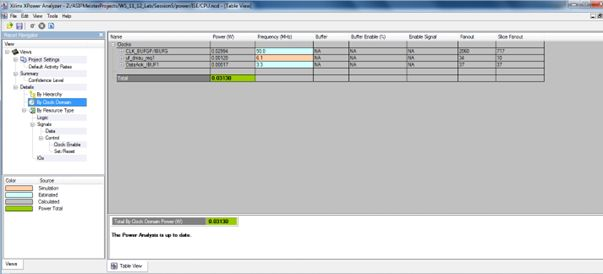
\includegraphics[width=0.9\textwidth]{src/images/7-3.png}
	\caption{Checking the CPU Frequency}
	\label{fig:fig73}
\end{figure}
To compare the power consumption between two processors, the average
value will not give correct information because every processor can
execute the same application with different execution time, as shown in Figure \ref{fig:fig73}. In this case, we need to consider
the energy. The energy is defined as the power consumed during whole
execution time, and given as:

E = P \textsubscript{*} T
\begin{figure}[!htb]
	\centering
	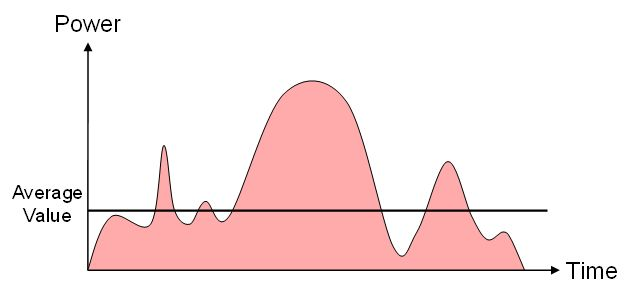
\includegraphics[width=0.9\textwidth]{src/images/7-4.png}
	\caption{Power Dissipation as Average Value}
	\label{fig:fig74}
\end{figure}
\begin{figure}[!htb]
	\centering
	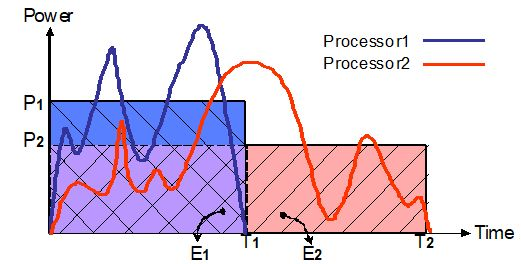
\includegraphics[width=0.9\textwidth]{src/images/7-5.png}
	\caption{Energy Comparison between two Processors}
	\label{fig:fig75}
\end{figure}
 
\hypertarget{extended-gcc-compiler}{%
\chapter{Extended GCC Compiler}\label{extended-gcc-compiler}}

The Extended GCC compiler development system is a compiler generator
that automatically creates an executable compiler out of an architecture
description. In our case, ASIP Meister automatically creates this
architecture description itself and an afterwards running program
provided by the developers of ASIP Meister. In this chapter, some basics
about the buildup of retargetable compilers, creation and usage of a GCC
compiler for our specific ASIP Meister CPU's are explained.

\hypertarget{basics-about-retargetable-compilers}{%
\section{Basics about Retargetable
Compilers}\label{basics-about-retargetable-compilers}}
\begin{figure}[!htb]
	\centering
	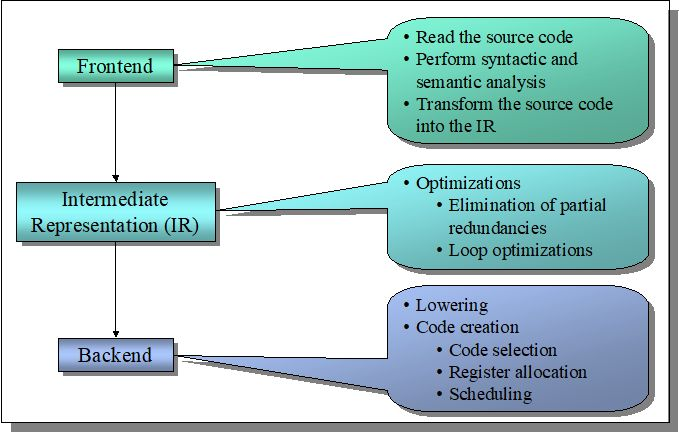
\includegraphics[width=0.8\textwidth]{src/images/8-1.png}
	\caption{A Typical Buildup for a Retargetable Compiler}
	\label{fig:fig81}
\end{figure}
A typical retargetable compiler like CoSy \cite{CoSy} is separated into \textbf{three} phases,
as shown in Figure~8‑1. The first stage is architecture independent, but
source language dependent. This phase reads the source code, inspects it
for syntactic and semantic correctness, and transforms it into the
second phase, the intermediate representation (IR). This IR is as well
source language independent as architecture independent and it is used
to perform the optimizations. This implies, that the optimizations can
be easily reused, if the source language or the architecture changes.
The third phase is source language independent, but highly architecture
dependent. This backend first transforms the IR into a low-level form.
That means, that high-level structures, like polymorphic procedure calls
are replaced by jump tables or that complex data structures are
disassembled into elementary memory accesses. Afterwards the final
assembly code has to be created. This part is separated into
\textbf{three} steps. In the first step, code has to be selected out of
the lowered IR. This code selection is not unique, as there are always
different possibilities to represent some statements in assembly
language. This code selection works with virtual registers, which are
replaced by real registers in the second step. This register allocation
might lead to additional stack accesses for swapping values out, if no
free real register can be found to hold the value of a virtual register.
In the third step, the code is scheduled, to minimize penalties for data
dependencies. Every step from this code selection has a great influence
on the outcome of the other steps. The sequence of these steps is not
determined and different compilers work with different sequences. The
above given order is just exemplary.

\hypertarget{creating-the-extended-gcc-compiler-in-asipmeister}{%
\section{Creating the Extended GCC Compiler in
ASIPmeister}\label{creating-the-extended-gcc-compiler-in-asipmeister}}

The ASIP Meister complier generation supports the base processor
Brownie. In order for the compiler to generate instructions that are
extended from the Brownie processor, some definitions are necessary.
Using {[}C Definitions{]}, you can define the C description
specifications that are supported by the ASIP Meister compiler and the C
description variables that support the instructions extended from the
Brownie processor. The ``Compiler Generation'' is possible only for the
processor extending a base processor Brownie. One can define how to
represent the extension instruction added to the base processor Brownie
in C code during the ``C Definition'' stage. Extension instruction
definition enables a complier to output assembly code complying with the
extension instruction.

\hypertarget{c-definition}{%
\subsection{C Definition}\label{c-definition}}

On the ``Ckf Prototype'' tab of ``C Definition'' sub-window in
ASIPmeister, you can define all the newly defined instructions as
described in the Page-65 of {[}TUT{]} and on the Page-57 of {[}UM{]}

\hypertarget{compiler-generation}{%
\subsection{Compiler Generation}\label{compiler-generation}}

At ``Compiler Generation'' stage in ASIPmeister, the processor compiler
and the Binutils can be generated. The processes involved in the
``Compiler Generation'' phase are as follows.

1. Input Description Generation: select and run.

2. GNU Tools Generation: select and run.

If you select ``Input Description Generation'' from the drop down list,
the compiler extended description will be generated. After the
generation terminates successfully, if the design data file was called''
browstd32.pdb'', a new directory called'' browstd32.swgen'' will be
generated inside ''meister'' directory, and inside this directory the
compiler extended description is generated in a file named ''
browstd32.xml''. The generated compiler and Binutils supports the Ckf
defined at ``C Definition''. After you select ``GNU Tools Generation''
and the generation terminates successfully, the compiler and the
Binutils will be generated in default directory called
''browstd32.swgen'' in the ``meister'' directory.

\hypertarget{using-custom-instruction-in-the-c-program}{%
\subsection{Using custom instruction in the C
Program}\label{using-custom-instruction-in-the-c-program}}

Once the custom instruction is defined in the ``C Definition'', they can
be used in the C program as described on the Page-63 in {[}UM{]} and on
Page-68 in {[}TUT{]}. There are two methods to use the custom
instruction here:

\begin{enumerate}
\def\labelenumi{\arabic{enumi}.}
\item
  When you want to write the extended instruction description in C code,
  you have to add ``\_\_builtin\_brownie32\_'' directive to the ``ckf
  definition''. An example is demonstrated in the following for a custom
  instruction AVG with three parameters (AGV rd, rs1, rs2).
\end{enumerate}
\begin{lstlisting}
int a=12,b=23,c;  
c = __builtin_brownie32_AVG(a, b);	
\end{lstlisting}
\begin{enumerate}
\def\labelenumi{\arabic{enumi}.}
\setcounter{enumi}{1}
\item
  In some cases, above method does not work, e.g., when an instruction
  returns a ``void''. Standard inline assembly directives can be used to
  write the extended custom instruction, as follows:
\end{enumerate}
\begin{lstlisting}
  __asm__ volatile (
"avg %[my_out], %[my_op1], %[my_op2]\n"
: [my_out] "=&r" (c)
: [my_op1] "r" (a),[my_op2] "r" (b)
);	
\end{lstlisting}
\hypertarget{using-the-extended-gcc-compiler}{%
\subsection{Using the Extended GCC
Compiler}\label{using-the-extended-gcc-compiler}}

In the lab, the Makefile is automatically doing all the steps. However,
you can also use the generated compiler separately; the following
demonstrates a method for cross compiling a C program file called
``bubble.c''.

\begin{enumerate}
\def\labelenumi{\arabic{enumi}.}
\item
  First, you have to add the path ``browstd32.swgen/bin'' to the \$PATH
  environment variable.
\end{enumerate}
\begin{lstlisting}
export COMPILER_DIR=/brownie/meister/browstd32.swgen/bin
or
export PATH=/brownie/meister/browstd32.swgen/bin:$PATH
\end{lstlisting}
\begin{enumerate}
\def\labelenumi{\arabic{enumi}.}
\setcounter{enumi}{1}
\item
  Compile the C program into .s assembly file
\end{enumerate}
\begin{lstlisting}
${COMPILER_DIR}/brownie32-elf-gcc -S -combine  -O3 bubble.c -o bub-ble.s	
\end{lstlisting}
\begin{enumerate}
\def\labelenumi{\arabic{enumi}.}
\setcounter{enumi}{2}
\item
  Assemble bubble.s file into .o object file. Also, assemble startup.s
  (startup code) and handler.s (interrupt handler) file to object files.
\end{enumerate}
\begin{lstlisting}
${COMPILER_DIR}/brownie32-elf-as -o startup.o startup.s;
${COMPILER_DIR}/brownie32-elf-as -o handler.o handler.s;
${COMPILER_DIR}/brownie32-elf-as -o bubble.o bubble.s;
\end{lstlisting}
\begin{enumerate}
\def\labelenumi{\arabic{enumi}.}
\setcounter{enumi}{3}
\item
  Link the object files using the linker script ``browtb.x''. This
  script declares some important information about the stack pointer,
  text and data sections, program counter address after the resetting
  the CPU.
\end{enumerate}
\begin{lstlisting}
${COMPILER_DIR}/brownie32-elf-ld -o bubble -T browtb.x bubble_uart.o startup.o handler.o
\end{lstlisting}
\begin{enumerate}
\def\labelenumi{\arabic{enumi}.}
\setcounter{enumi}{4}
\item
  Converting compiled object file to memory image of the C program. Use
  ``gccout2img'' for a file in elf format obtained through normal
  compilation. The script ``gccout2img'' outputs \emph{TestData.IM} and
  \emph{TestData.DM}, with which the user can perform simplified test
  simulations.
\end{enumerate}
\begin{lstlisting}
gccout2img bubble	
\end{lstlisting}
\hypertarget{library-with-standard-functions-for-asip-meister-gcc-hardware-prototype}{%
\section{Library with Standard Functions for ASIP Meister / GCC /
Hardware
Prototype}\label{library-with-standard-functions-for-asip-meister-gcc-hardware-prototype}}

Many applications use some standard library calls like \emph{printf},
\emph{malloc} or \emph{atoi} that are not declared in the standard of
the C programming language, but which are nevertheless declared in the C
standard library. Now, GCC is a compiler for the C language and does not
provide an implementation for the standard library (in fact there are
some huge fragments that would have to be adapted to our specific
environment, what has not been done due to the complexity of a full
run-time implementation).

To close the gap between a plain C compiler and the wish of letting
complex algorithms run in hardware and produce understandable output we
are providing some basic \emph{stdlib} functionality, which is dedicated
to the environment of ASIP Meister, the GCC compiler and our hardware
prototype. This basic \emph{stdlib} functionality is extended on demand
to reflect the latest changes of our environment. Thus, it is not
explained exhaustively or in high detail. Instead, the underlying
concepts and the needed steps for using the basic \emph{stdlib} library
is explained here, plus some of the main functions for using our touch
screen LCD with some examples.

All typical functionalities of our \emph{stdlib} implementation are
available in the directory \emph{/home/asip00/epp/StdLib/.} The
functionality is encapsulated into a header file that is providing the
interface and a documentation of the functionality and a C file for
implementing the header. You can use these files by linking/copying them
into your application project subdirectory and using ``\emph{make sim}''
to compile your application and the \emph{stdlib} files into one binary
and simulation file, as it will be shown in the example below. Linking
to the files instead of copying them has the advantage, that you always
have the latest version of these files in your project. Some of the
files in the \emph{stdlib} directory have dependencies to other files of
this directory. Thus, you can get a compiler error, that a specific
header file was not found when you try to compile your project. You then
have to manually link to the dependent files as well. Just linking to
all available files is generally not a good idea, as this makes the
compilation process take longer and it increases the needed memory size
of your application.

Now we will demonstrate how you can create a small application that is
using the LCD of the hardware prototype:
\begin{itemize}
\item
  Create a new subdirectory inside the application directory of your
  ASIP Meister project and change into this new directory
\item
  Copy or Link to \emph{lib\_lcd}, \emph{loadStorByte} and
  \emph{string}, by executing:
\begin{lstlisting}
	ln -s /home/asip00/epp/StdLib/lib_lcd_320.* .
	ln -s /home/asip00/epp/StdLib/loadStoreByte.* .
	ln -s /home/asip00/epp/StdLib/string.* .	
\end{lstlisting}
\end{itemize}
\begin{quote}
\emph{lib\_lcd} has a dependency to \emph{loadStoreByte} and
\emph{string}, that is why you need both.

The \emph{lib\_lcd\_320} exists in different C implementations,
depending on your target LCD. One C file is for the LCD with a 240x128
resolution, the other one is for the 320x240 resolution, and the last
one is for the dlxsim simulation. Make sure that at most, one of these C
files is available in your application subdirectory; otherwise, the
linker will complain about multiple implementations (one per C file) of
the LCD functionality.
\end{quote}

\begin{itemize}
\item
  Prepare an ``\emph{env\_settings}'' file, as shown in Chapter~6.4.
\item
  Add a new C file that contains your main method. This main method will
  contain the following code as example:
  \begin{lstlisting}
 	t_print("Hello World\r\n");
 	t_printInt(42);
  \end{lstlisting}
\end{itemize}
\begin{quote}
The LCD needs the ``\emph{\textbackslash r\textbackslash n}'' in the
string, as it is handling carriage return (\textbackslash r) and line
feed (\textbackslash n) independently.
\end{quote}

\begin{itemize}
\item
  Compile your project by executing ``\emph{make sim}''.
\end{itemize}

The resulting program can be simulated with dlxsim or ModelSim or it can
be uploaded to the hardware prototype (explained in Chapter~6.4)
depending on the selected LCD library.

After you have once compiled a C-Code that rarely changes (e.g. the
libraries), you can reuse the created assembly code for future
compilations. That will enormously speed up the whole compilation
process. This is especially good for all applications in the
\emph{StdLib} directory. Just compile them one time with ``\emph{make
sim}'' and then copy the created .\emph{asm} file from the
``\emph{BUILD\_SIM}'' directory to the directory of your other
application files, but name it .s instead of .asm. Then remove the C
code (but not the header) to make sure the code does not exist twice (in
the C code and in the Assembly file). For instance:
\begin{lstlisting}
cp BUILD_SIM/loadStoreByte.asm loadStoreByte.s
rm loadStoreByte.c	
\end{lstlisting}
However, when moving from dlxsim to FPGA implementation then you have to
delete these assembly files, link to the C files, and recompile them. If
you are often switching between dlxsim and FPGA, then it may be
beneficial to create two application directories with the different
libraries and ``\emph{env\_settings}'' specified for dlxsim and FPGA
respectively and using the same application-specific source code in both
directories (e.g. with a link).

As mentioned above, the ``\emph{lib\_lcd}'' exists in different
variants. The files ``\emph{lib\_lcd\_240.c}'' and
``\emph{lib\_lcd\_320.c}'' are for the FPGA prototype. They implement
the real protocol for communicating with the I\textsuperscript{2}C bus
and thus with the LCD. For a simulation, we cannot use this
implementation, as it is waiting for certain responses from
I\textsuperscript{2}C/LCD, but in dlxsim/ModelSim simulation, these
answers will never appear. We have therefore implemented
``\emph{lib\_lcd\_­dlxsim.c}'' which simply writes every single
character that is send to the LCD to an output file (a virtual LCD).
This is a very good debugging possibility for printing text, although it
is not helpful for any graphic output to the LCD (e.g. lines, bars
\ldots), as these control words are hard to understand manually. For
dlxsim, the characters are either printed to the console whenever they
appear or they are collected and printed to a file (parameter ``-lf'' in
Chapter~3.2.1). For ModelSim, the characters are printed to a file
``\emph{lcd.out}'' in the ModelSim directory. The header file
``\emph{lib\_lcd.h}'' is valid for all C files, but you have to make
sure, that at most one of the both C files is available in the directory
when compiling with ``\emph{make sim}''. Otherwise, you will get two
implementations of the LCD functions and the assembler will complain,
that he cannot decide which one to choose.

\hypertarget{functions-of-the-lcd-library}{%
\subsection{Functions of the LCD
Library}\label{functions-of-the-lcd-library}}

This chapter summarizes some of the available functions to access the
features of the LCD of our hardware prototyping board. The library also
contains some high-level functionality that is useful, but introduces a
dependency to ``\emph{string.c}''. Therefore, this library has to be
provided as well when using ``\emph{lib\_lcd}''.

The most important basic I/O instructions are:
``\emph{t\_print(char*)''}, ``\emph{t\_printInt(int)''}, and
``\emph{t\_printHex(int value, int digits)''}. You can use them to print
strings and numbers, for instance:
\begin{lstlisting}
char tempString[] = "\r\n\t\t";
t_print("Hello World!");
t_print(tempString);
t_printInt(23);
t_print(" = ");
t_printHex(23, 0);
t_print(tempString)
t_printInt(42);
t_print(" = ");
t_printHex(42, 4);	
\end{lstlisting}
The ``\emph{printHex()''} function can trim the output to a given number
of digits (4 in this case). To not trim the number of digits you have to
give `0' as parameter. The output of the above example looks like:
\begin{lstlisting}
Hello World!
	23 = 0x17
	42 = 0x002A	
\end{lstlisting}
In the following, we describe further functions of the LCD. Some of them
are generally sending a command to the LCD (you have to use the LCD
manual \cite{eDIP} to find the available commands) and some of them are
offering typical commands (e.g. \emph{drawline}) as convenience
functions.
\begin{lstlisting}
int checkbuffer()
\end{lstlisting}
This function returns the number of available bytes in the send buffer
of the LCD. It can be used to wait for a return value of the LCD. For
example when pressing a button on the touch panel, a value of this
button is written to the LCD send buffer.
\begin{lstlisting}
int getbytes (char* dest, int bytes_to_read)
\end{lstlisting}
This reads a specific number of bytes from the send buffer. With the
``\emph{checkbuffer''} function, you can test how many bytes are
available in the buffer.
\begin{lstlisting}
int sendcommand (	const char cmd0, const char cmd1, const int options[], const char text[],
int intcount, int charcount, int address)
\end{lstlisting}
This is a general function for sending commands to the LCD. The
following commands internally use ``\emph{sendcommand''} to realize
their functionality. The parameters of ``\emph{sendcommand''} are:

\begin{itemize}
\item
  Two chars, specifying the command
\item
  Depending on the type of the command, some options
\item
  Depending on the type of the command a string with a predefined size
\item
  The address of the LCD (defined in \emph{lib\_lcd.c})
\end{itemize}
\begin{lstlisting}
int t_print (const char* str)
\end{lstlisting}
This function writes a string to the LCD terminal. The ``\emph{t\_}''
indicates a command for the console mode of the LCD, compared to the
graphic mode (\emph{g\_}) of the LCD, which is explained later.
\begin{lstlisting}
int t_cursor (int onoff)
\end{lstlisting}
Turns on (1) or off (0) the blinking cursor of the terminal.
\begin{lstlisting}
int t_enable (int onoff)
\end{lstlisting}
Turns the display on (1) or off (0). When the display is turned off, all
submitted data is ignored. Previously sent data (when the display was
on) is buffered and will become visible again, after the display will
become turned on again.
\begin{lstlisting}
int g_print (const char* str, int x, int y)
\end{lstlisting}
Writes a string to the coordinates (x, y). You must not send control
signals like \textbackslash n in this function. They are only available
for the t\_print function.
\begin{lstlisting}
int g_drawrect (int x1, int y1, int x2, int y2)
int g_drawline (int x1, int y1, int x2, int y2)	
\end{lstlisting}
Draws a rectangle/line.
\begin{lstlisting}
int g_makebar (	int x1, int y1, int x2, int y2, int low_val, int high_val, int init_val, int type, int fill_type, int touch)
\end{lstlisting}
Creates a bar graph at the defined coordinates. ``\emph{low\_val''} and
``\emph{high\_val''} describe the minimal and maximal (at most 254)
value of the bar graph. ``\emph{init\_val''} defines the initial value
and ``\emph{type''} and ``\emph{fill\_type''} adjust the appearance of
the graph. Type=1 will draw a bar in a box and the ``\emph{fill\_type}''
(in the range of 1 to 15) then defines the fill pattern. Type=3 will
draw a line in a box and the ``\emph{fill\_type}'' will then define the
thickness of the line. For more details refer too {[}LCD{]}.

With ``\emph{touch''} you can define, whether the bar graph will be user
changeable by the touch screen. Every bar graph gets a unique number,
which is returned by the function. At most 32 bar graphs are supported
by the display. When the touch screen functionality is activated and the
user changes the value of the bar graph, the LCD automatically writes
the number of the changed bar graph and its modified value to the
buffer, from where it can be received with the checkbuffer and getbytes
function.
\begin{lstlisting}
int g_setbar (int barnum, int value)
\end{lstlisting}
Sets an existing bar graph to a specific value.
\begin{lstlisting}
int g_makeswitch ( const char* str, int x1, int y1, int x2, int y2, int
down, int up)	
\end{lstlisting}
Creates a switch (button) with a label. The parameter ``\emph{str''}
contains this label, preceded by a control char which defines the
alignment of the label. ``C'' means centered, ``L'' means left- and
``R'' means right-aligned. \emph{down} and \emph{up} define the code,
which the LCD will write into the send buffer, when the button is
pressed or released. When 0 is provided as parameter for up or down,
then nothing will be written to the buffer for the specific activity.
\begin{lstlisting}
int g_makeradiogroup (int group_number)
\end{lstlisting}
A new defined switch can be assigned to a specific radio group. A radio
group automatically makes sure, that at most one switch of the group is
pressed.
\begin{lstlisting}
int g_makemenubutton ( const char* str, int x1, int y1, int x2, int y2,
int down, int up, int select, int space)	
\end{lstlisting}
A menu item is created. With ``\emph{str''} you can define the
appearance and the menu entries. The first character defines the
direction in which the menu will open (``L'': left, ``R'': right, ``O''
up, ``u'': down). The second char defines the alignment of label on the
menu item (``C'': centered, ``L'': left aligned, ``R'': right aligned).
The labels of the menu entries follow afterwards and are separated by a
``\textbar'' sign. ``\emph{down''} defines the value that will be
written to the buffer, when the menu item is pressed and up defines the
value that will be written to the buffer, when the menu is closed,
without choosing a specific entry (aborted). ``\emph{select''} defines
the base value that is used to compute the value that will be written to
the LCD buffer, when a menu entry is chosen. This value is computed as:
base value~+~entry number~--~1. ``s\emph{pace''} defines the gap in
pixels between the menu entries. This is a global value, thus it will
also change the appearance of already existing menus.

\hypertarget{functions-of-further-libraries}{%
\subsection{Functions of Further
Libraries}\label{functions-of-further-libraries}}

Besides the LCD, further functionality and helping functions are
available. They will be summarizes in this section to give an overview
of the available features. You should look into the libraries to find
out more.

\textbf{lib\_uart:} besides printing to LCD, you may also print to the
UART port using the ``\emph{u\_print''}, ``\emph{u\_printInt''}, and
``\emph{u\_printHex''} functions (similar to ``\emph{t\_print''} etc.).
You can read from the UART port with ``\emph{u\_getbytes''}. However,
you need a HyperTerminal running at the pc to which the UART is
connected (see Chapter~6.4.2 for details about the HyperTerminal). In
Modelsim, uart.out is automatically created while for dlxsim you can
pass the parameter ``-uf'' to print text in a file instead of appearing
on the console.

\textbf{lib\_audio:} you can write uncompressed PCM audio data to an
audio port using the ``\emph{audioAddressR\{L\textbar R\}}'' pointers.
The corresponding sample width of the corresponding IP core in the
VHDL-framework (default 16 Bit) can be configured in
``\emph{AudioOut\_Types.vhd''} and the sampling rate (default 40 KHz)
can be configured in ``\emph{dlx\_Toplevel.vhd''} (search for
`i\_audio\_out').

\textbf{lib\_clock:} you can use the pointer ``\emph{clockAddress}'' to
read and write to access a special register that automatically
increments by one in each cycle. You can use this to benchmark the
performance of a certain C-Code by e.g. writing a `0' to it to start the
benchmark and to read it again at the end of the benchmark. Make sure
that the code that will be benchmarked does not contain any unnecessary
I/O instructions (e.g. ``\emph{t\_print''}) as they are extremely slow.

\textbf{String:} contains some typical string manipulation functions,
e.g. ``\emph{strlen''}, ``\emph{strcat''}, ``\emph{strcpy''} \ldots{} It
additionally contains two functions to convert an integer number to a
string representation, as it is used in the I/O libraries, e.g.
``\emph{t\_printInt''} or ``\emph{u\_printHex''}.

\hypertarget{changing-the-frequency}{%
\subsection{\texorpdfstring{Changing the Frequency
}{Changing the Frequency }}\label{changing-the-frequency}}

In order to change the frequency of your design and see if it still
works or not (required for the last Session), the Framework contains a
DCM (Digital Clock Manager) that generates five different clocks. By
changing the knob on the external PCB, a multiplexer (in the
``dlx\_toplevel.vdh'' file) selects the corresponding frequency that you
want to apply on your design.
\begin{table}[!htb]
	\centering
	\begin{tabular}{|c|c|}
		\hline
		\textbf{Knob value} & \textbf{Frequency (MHz)} \\ \hline
		0                   & 100                      \\ \hline
		1                   & 80                       \\ \hline
		2                   & 66                       \\ \hline
		3                   & 50                       \\ \hline
		4                   & 40                       \\ \hline
		5                   & 25                       \\ \hline
		Else                & 100                      \\ \hline
	\end{tabular}
	\caption{Knob Position \& Corresponding Frequencies}
	\label{fig:fig82}
\end{table}
 
%\chapter{Background}
\label{ch:Background}
  
%\chapter{Machine Learning for Hardware Security}

%\chapter{Summary}
\label{ch:Summary} 
%Generate list of figures and tables
\listoffigures
\listoftables
%Add list of figures and tables Section into ToC
\addcontentsline{toc}{chapter}{List of Figures} 
\addcontentsline{toc}{chapter}{List of Tables}
%% ----------------
%% |   Appendix   |
%% ----------------

\appendix
%\include{src/appendix/anhang_a}
%\include{src/appendix/anhang_b}

%% --------------------
%% |   Bibliography   |
%% --------------------

\cleardoublepage
\phantomsection
\addcontentsline{toc}{chapter}{\bibname}
\printbibliography


\end{document}
%% --------------------------------------------------------------------------------
%% |                              END OF DOCUMENT                                 |
%% --------------------------------------------------------------------------------